% ---- ETD Document Class and Useful Packages ---- %
\documentclass{ucetd}
\usepackage{subfigure,epsfig,amsfonts}
\usepackage{natbib}
\usepackage{amsmath}
\usepackage{amssymb}
\usepackage{amsthm}
% Add extra packages I need
% Packages used by pandoc when converting Markdown to LaTeX
\usepackage{fixltx2e}
\usepackage{longtable}
\usepackage{booktabs}
% Make cross-references hyperlinks (also format URLs with \url).
% Specify breaklinks so that titles in table of contents linewrap.
\usepackage[breaklinks]{hyperref}
% Fix to use hyperref with UCETD template (from Jason Torres)
\renewcommand{\etdChapterHeadFormat}[1]{\uppercase{#1}}
% Ability to split long captions across pages
\usepackage{ccaption}
% Crop figures
\usepackage{graphicx}
% Add footnote to List of Tables about the supplementary files
\renewcommand{\listtablename}{List of Tables
  \footnote{Note: Due to the large size of some tables, the tables
  have been provided in a supplementary file accompanying the
  dissertation. In such cases, the page number provided below directs
  the reader to a table's caption.
}}
% Nice tilde
% http://tex.stackexchange.com/questions/9363/how-does-one-insert-a-backslash-or-a-tilde-into-latex/9372#comment47661_9372
\newcommand{\mytilde}{\raise.17ex\hbox{$\scriptstyle\mathtt{‌​\sim}$}}


%% Use these commands to set biographic information for the title page:
\title{The Role of Alternative Polyadenylation Variation in Gene Regulation Differences Within and Between Species}
\author{Briana Erin Mittleman}
\department{Genetics, Genomic, and Systems Biology}
\division{Biological Sciences}
\degree{Doctor of Philosophy}
\date{August 2020}

%% Use these commands to set a dedication and epigraph text
\dedication{Dedication Text}
\epigraph{Epigraph Text}


\begin{document}
%% Basic setup commands
% If you don't want a title page comment out the next line and uncomment the line after it:
\maketitle
%\omittitle

% These lines can be commented out to disable the copyright/dedication/epigraph pages
\makecopyright
%\makededication
%\makeepigraph


%% Make the various tables of contents
\tableofcontents
\listoffigures
\listoftables

% Enter Acknowledgements here
\acknowledgments


To complete:

Yoav
Seb
Yang
Gilad lab
Other grad school people 
friends 
family
funding...

chicago things- 
trapeze
OTF hyde park 
edgewater starbucks 

fenway

% Enter Abstract here
\abstract

Differences in gene regulation contribute to phenotypic differences within humans and also between humans and other primates. While co-transcriptional gene regulatory mechanisms such as alternative polyadenylation \emph{(APA)} can help explain how variation in gene regulation manifests, such mechanisms remain understudied. In this thesis, I used a quantitative genomics approach and a comparative primate approach to understand the regulatory role of APA. In chapter 2, I measured polyadenylation site \emph{(PAS)} usage genome wide in a population of 52 human lymphoblastoid cell lines. I identified genetic variation associated with APA \emph{(apaQTLs)} and showed that genetic variation acts through PAS choice to impact mRNA expression, translation, and protein levels in complex, non-linear ways. In chapter 3, I measured APA conservation between human and chimpanzee. While APA is largely conserved, differences in PAS usage and isoform diversity contribute to differentially expressed and differentially translated genes. Together, these chapters, establish APA as a key co-transcriptional mechanism underlying the genetic regulation of gene and protein expression levels. As a step to further understand co-transcriptional regulatory mechanisms, in chapter 4, I describe an attempt to measure polymerase II elongation rate genome wide. In the final chapter, I outline a set of necessary future directions to extend my work on APA to more tissues and biological processes.
\\
\\
 (Note:
Supplementary tables are provided in a .zip file available
online. Captions for the tables are provided within the dissertation.)


\mainmatter
% Main body of text follows

% Chapter 01 - Introduction
\chapter{Introduction}

An overarching goal in human genetics is to understand the relationship between genotype and phenotype. An integral step toward this goal is learning how to interpret the functional consequences of genetic variants. In protein-coding regions, it is relatively easy to predict if a single nucleotide polymorphism \emph{(SNP)} will affect protein sequence because the amino acid code is known. However, protein-coding genetic sequence makes up only $\sim1$\% of the genome. Although non-coding regions of the genome were categorized as "junk DNA" for decades, it is now clear that a large proportion of the non-coding genome is essential. Indeed, non-coding DNA has been established to play a large role in gene regulation - the chain of events controlling how and when cells express particular genes. Thus, understanding how non-coding genetic variants influence gene regulation is a vital step toward understanding the relationship between genotype and phenotype. 

In this chapter, I will introduce the two approaches that I have taken in my work to study gene regulation. By providing examples, primarily from the Gilad lab, I will motivate why I have chosen to study gene regulation through quantitative genetics and comparative primate functional genomics. Following this discussion, I argue that co-transcriptional gene regulatory mechanisms remain understudied and warrant particular attention by both approaches. I conclude the chapter with an overview of the remaining chapters in this dissertation.  


\section{Quantitative genetic approaches to understand gene regulation}

Quantitative trait loci \emph{(QTL)} mapping is a tool used to identify genetic variation affecting gene regulation. For example, an expression QTL, or eQTL, is a genetic variant that is statistically associated with mRNA expression.  Over the last decade, a large number of eQTL mapping studies have identified genetic variants with regulatory potential in a wide range of human cell lines and tissues \citep{lappalainen_transcriptome_2013, stranger_population_2007, stranger_population_2007, pickrell_understanding_2010, gtex_consortium_genetic_2017, schmiedel_impact_2018}. In the most comprehensive project to date, the Genome-Tissue Expression \emph{(GTEx)} Consortium generated eQTL maps for over 50 human tissues collected from over 800 healthy individuals \citep{ward_cracking_2017, aguet_gtex_2019, gtex_consortium_genetic_2017}. Integration of these maps has revealed numerous eQTLs for the majority of protein coding genes.  

While eQTLs have been largely successful in identifying SNPs with regulatory potential, this approach does not reveal the chain of events controlling gene expression levels. eQTLs represent a collection of SNPs mediating gene expression along the gene regulatory cascade through a wide range of mechanisms \ref{fig:eQTLMech} \citep{Pai2015}. The development of methods like DNAse-seq \citep{song_dnase-seq_2010} ChIP-Seq \cite{barski_high-resolution_2007}, and ATAC-seq \citep{buenrostro_atac-seq_2015}, which are used to identify chromatin states, made it possible to study the contribution of specific molecular mechanisms to variation in gene expression levels. For example, if we assume an eQTL acts by perturbing a particular mechanism (i.e. chromatin conformation), the SNP should also be associated with measures of that mechanism, and molecular QTL mapping further contributes to the understanding of gene regulation. 


\begin{figure}
\centering
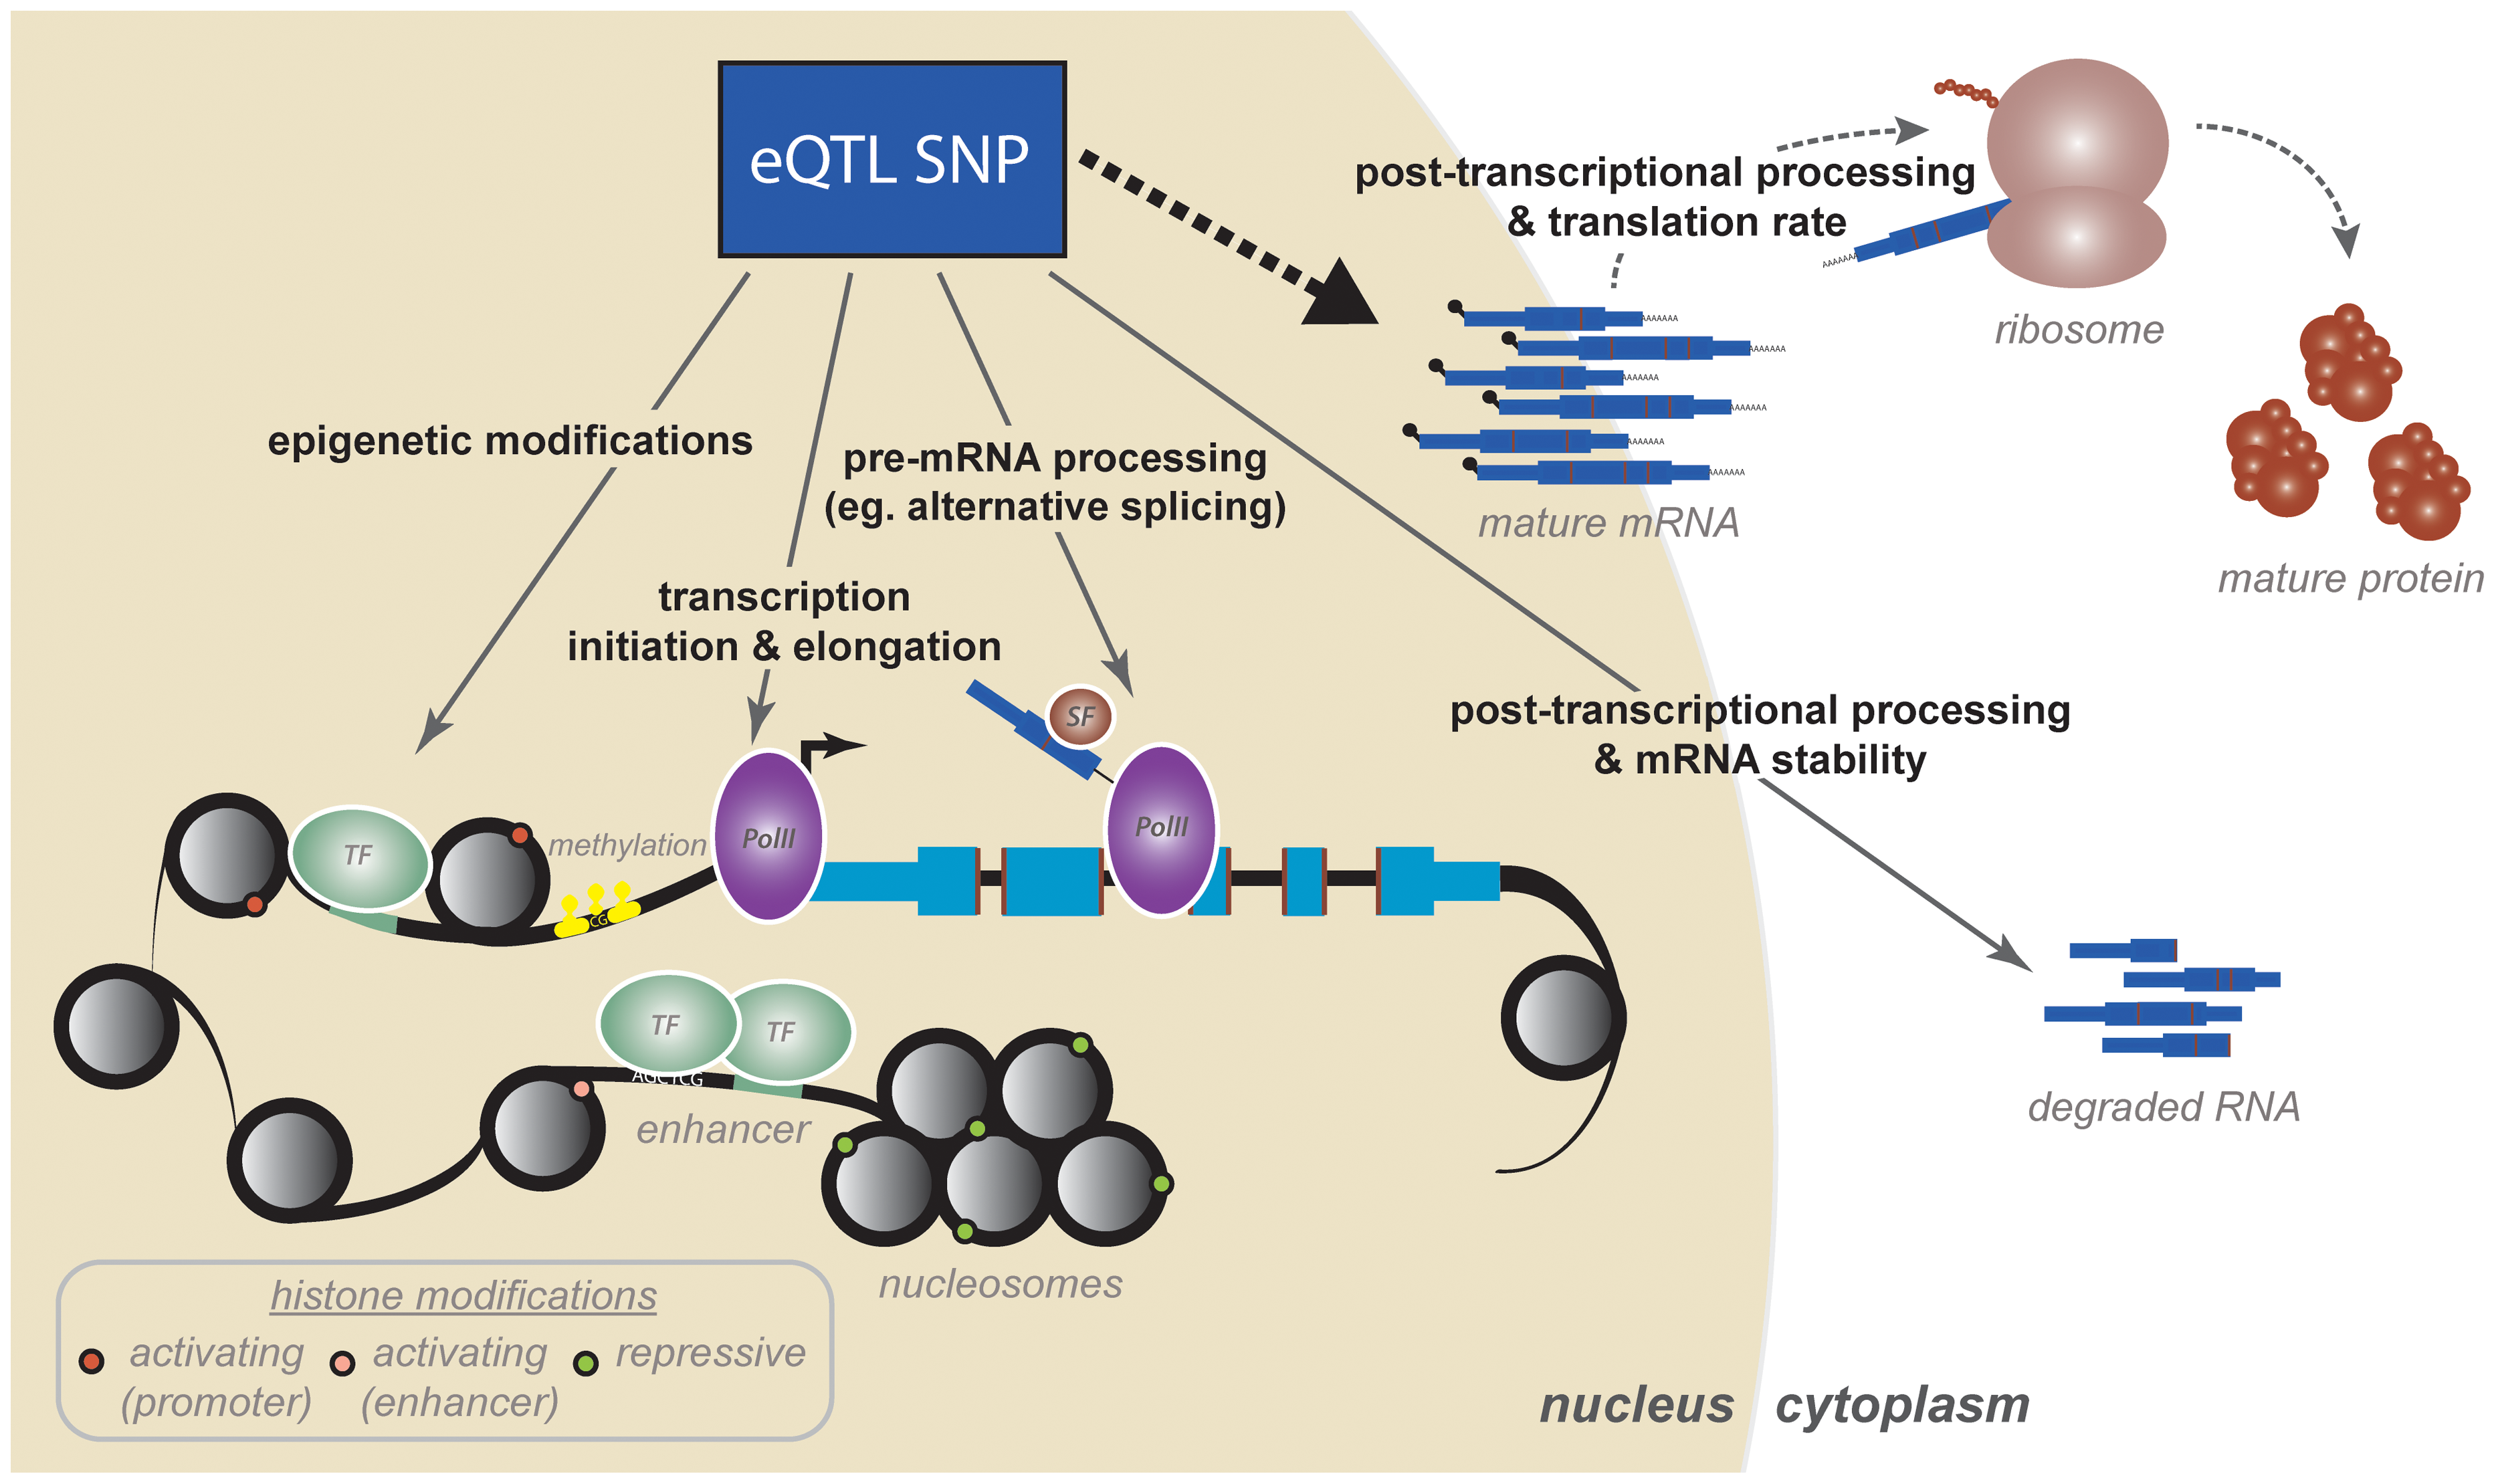
\includegraphics[width=5in]{img/ch01/eQTLMech.png}
\caption[Potential mechanisms for eQTLs]{Figure 1 from Pai, Pritchard, and Gilad 2015 \citep{Pai2015} Regulatory QTL studies have revealed how eQTLs can affect variation in mature mRNA expression levels as well as how variation in mRNA expression may then impact post transcriptional and translational mechanisms.} 
\label{fig:eQTLMech}
\end{figure}

\section{Comparative approaches to understand gene regulation}

Comparative primate functional genomic studies have also contributed to our understanding of human gene regulation. Like phenotypic variation between individual human, phenotypic differences between human and non-human primates stem largely from differences in gene regulation \citep{King1975, carroll_evolution_2005, gilad_expression_2006, wray_evolutionary_2007, blekhman_gene_2008, karaman_comparative_2003}. In turn, primate functional genomic studies complement human-specific quantitative genetic studies. Due to the challenges associated with obtaining primate tissues, comparative studies in primates typically rely on smaller sample sizes. However, these are sufficient to detect the large differences in regulatory mechanisms between species. Comparative genomic approaches also contextualize gene regulatory mechanisms in an evolutionary framework to provide additional insight into which processes or loci are critical to genome and organismal function. 

There are some regulatory processes that, while functionally important, are indistinguishable in human populations or are measured with technology not feasible to use at the scale necessary for quantitative genetic studies. Because genetic variation is larger between species than within human populations, it is possible to distinguish differences in regulatory features between species - even with small sample sizes. For example, before it became technically and financially feasible to measure chromosome contacts genome-wide at a human population level, Eres \emph{et al.} demonstrated that differences in contact frequencies at individual loci between human and chimpanzee can explain previously identified differentially expressed genes \citep{eres_reorganization_2019}. Specifically, Eres \emph{et al.} used Hi-C to characterize 3D chromatin contacts in human and chimpanzee induced pluripotent stem cells \emph{iPSCs}. While a quantitative genetics study to detect genetic variation associated with significant differences in chromatin interactions between humans was not feasible, this work demonstrated that chromatin contact variation likely mediates differences in gene expression, and complemented previous work that suggested direct contact between distal enhancer elements and promoters driving gene expression \citep{carter_long-range_2002, krivega_enhancer_2012, tolhuis_looping_2002, palstra_-globin_2003, marsman_long_2012}.

Comparative primate genome studies also provide evolutionary context for genetic mechanisms and genomic loci previously studied with alternative approaches. Under the assumption that conserved processes and loci are critical to function, understanding evolutionary context of gene regulatory mechanisms can help catalog importance of each mechanism \citep{housman_prime_2020}. For example, human quantitative genetics approaches revealed higher variation in mRNA transcript levels than protein levels, which likely result from mechanisms downstream of translation buffer protein levels \citep{battle_impact_2015}. However, the importance of post-translational gene regulation for maintaining protein level variation was unclear. Wang \emph{et al}, measured translation in a set of primate LCLs with available mRNA expression and protein levels. Using these data, the authors demonstrated that post-translation protein buffering likely plays a large role in shaping primate protein level divergence \citep{wang_post-translational_2018}. Overall, characterizing gene regulatory mechanisms in both humans and non-human primates is critical to understanding the broader relationship between genotype and phenotype. 

\section{Open questions in how isoform diversity contributes to gene regulation}

Both human population genomic and primate comparative genomic approaches have improved our ability to interpret noncoding variation, yet more work is necessary to understand the gene regulatory code.  It has become clear that a large number of highly conserved genetic variants that correlate with variation in both mRNA expression and complex traits lie in cis-regulatory elements such as promoters and enhancers \citep{maurano_systematic_2012, Trynka2013, zhou_epigenetic_2014}. While considerable effort has been devoted to annotating promoters and enhancers across cell types and species \citep{bernstein_nih_2010, the_encode_project_consortium_integrated_2012, mouse_encode_consortium_encyclopedia_2012, modencode_consortium_unlocking_2009}, a large proportion of variants associated with gene expression variation and/or complex traits remain unannotated and unexplained.

Indeed, the majority of previously explored gene regulatory mechanisms affect gene expression levels pre-transcriptionally through chromatin level variation at promoters and enhancers. However, co-transcriptional mechanisms, such as alternative mRNA splicing and alternative polyadenylation \emph{(APA)}, contribute to both variation in mRNA and protein isoforms dependent on and independent of changes in mRNA expression levels. Understanding the co-transcriptional mechanisms that mediate isoform diversity is a key path forward to predicting phenotype from genotype.  Thus, a greater understanding of how genetic variation and regulatory elements control alternative splicing and APA will fill a gap in predictive models of gene regulation from DNA sequences.

In recent years, a number of groups have started to identify and characterize the genetic variation associated with alternative splicing \emph{(sQTLs)} \citep{takata_genome-wide_2017, li_rna_2016, ongen_alternative_2015, ma_splicing_2018, tian_cancersplicingqtl_2019}. In one such study, Li \emph{et al.} mapped sQTLs in a population of LCLs that was previously used to characterize a number of other molecular QTLs. They reported that most sQTLs, including some previously implicated in GWAS, are not eQTLs \citep{li_rna_2016}. This work suggests genetic variation can mediate traits independently from differences in mRNA expression levels. 

Although comparative functional genomic studies of alternative splicing are still rare, a few studies have generated important insights. Blekhman \emph{et al.} reported that genes with human-specific exon usage are enriched in genes involved in anatomical structure \citep{blekhman_sex-specific_2010}. Additional work has demonstrated how alternative splicing may contribute specifically to differential expression and translation of genes between closely related primates \citep{lin_evolution_2010, attig_splicing_2016}. For example, Attig \emph{et al.} reported that co-evolution of splice sites and U-rich elements in primates has led to an increase in expression of exons containing Alu transposable elements. Their experiments demonstrated inclusion of Alu exons causes down regulation of transcripts through non-sense mediated decay \cite{attig_splicing_2016}.

 Like alternative splicing, cleavage and polyadenylation in introns leads to differential inclusion of coding sequences. mRNA transcripts resulting from intronic polyadenylation are either subject to decay or are translated to distinct protein isoforms (reviewed in Tian and Manley \citep{tian_alternative_2017}). Unlike alternatively spliced transcripts, APA in 3' untranslated regions (3' UTRs) produces transcripts with the same coding sequences thus only differing in 3' UTR length. Variation in downstream regulation of 3' UTR APA isoforms result from differential inclusion of miRNA binding sites and other motifs signaling RNA binding proteins. Thus, isoforms with distinct 3' UTRs are subject to alternative stability, localization, and translation (reviewed in Tian and Manley \citep{tian_alternative_2017}).
 
While the molecular basis for cleavage and polyadenylation of mRNA transcripts is known, the precise mechanisms that discriminate between potential polyadenylation sites \emph{(PAS)} in the same gene are not. Molecular biology studies have characterized the DNA motifs and the cascade of events leading to cleavage and polyadenylation of mRNA molecules \citep{takagaki_four_1989, colgan_mechanism_1997, macdonald_64-kilodalton_1994}. In short, elongating RNA polymerase II recognizes a canonical signal motif \emph{(AATAAA)} and recruits the necessary protein complexes to cleave the mRNA transcript and add adenosine bases to the 3' end. In turn, it is not surprising that studies have identified individual loci whereby signal site changes contribute to variation in APA and downstream regulation. However, over 80\% of human genes that have multiple isoforms do not contain signal sites changes that could directly point to differential usage of individual isoforms.

Variation in APA has been linked to functional regulatory changes that contribute to differences in complex traits and disease risk. For example, a genetic variant in the signal site of a PAS in the \emph{IRF5} gene has been causally linked to risk of systemic lupus erythematosus \emph{(SLE)} \citep{graham_three_2007}. Individuals with SLE have a genetic mutation that reduces the use of the most 5' proximal PAS in the 3' UTR of \emph{IRF5}. Usage of the distal PAS produces a longer 3' UTR with an AU-rich destabilizing element \emph{(ARE)}. As a result, the alternative isoform is quickly degraded, reducing gene expression of IRF5 in these patients. However, the role of APA in gene regulation and disease risk genome-wide remains understudied.

By gaining a more complete understanding of the genetic basis for PAS choice and the level of PAS usage conservation in primates, it will be possible to place APA into complex models of gene regulation. It is likely that genetic variation associated with APA \emph{(apaQTLs)} will both help to explain eQTLs outside of enhancers and promoters as well as GWAS loci not previously associated with eQTLs. Variation in APA may also contribute to how genes are differentially expressed between humans and non-human primates at both the mRNA and protein levels.

The goal of my work is to begin to characterize APA in populations of humans and non-human primates in an experimentally tractable cell type. I have ensured the methods and analysis pipelines are available for others so that they can expand this important work to a wider range of cell types and biological processes. Together these studies will contribute to the understanding of non-coding genetic variation and the molecular processes connecting genotype to phenotype.


\section{Dissertation overview} 

The work I will present in this dissertation aims to characterize the role of APA in gene regulation. In chapter \ref{ch:QTL}, I take a quantitative genetic approach by identifying genetic variation associated with APA in a panel of 52 human lymphoblastoid cells lines \emph{(LCLs)}. In chapter \ref{ch:comp}, I use a comparative primate genomics approach to identify both conserved and divergent cases of APA between human and chimpanzee. In chapter \ref{ch:netseq}, I describe an attempt to understand how transcription dynamics contributes to variation in both alternative splicing and APA. Finally, in chapter 5, I conclude the dissertation by placing my work in context with other recent work in the area and describe my recommendations for future directions. 


% Chapter 02
% Chapter 02
\chapter{Alternative polyadenylation mediates genetic regulation of gene expression}\label{ch:QTL}
\section[Abstract]{Abstract\footnotemark}


%\ref{fig:response-eqtl}. 

Little is known about co-transcriptional or post-transcriptional regulatory mechanisms linking noncoding variation to variation in organismal traits. To begin addressing this gap, we used 3' Seq to study the impact of genetic variation on alternative polyadenylation (APA) in the nuclear and total mRNA fractions of 52 HapMap Yoruba human lymphoblastoid cell lines. We mapped 602 APA quantitative trait loci (apaQTLs) at 10\% FDR, of which 152 were nuclear specific. Effect sizes at intronic apaQTLs are negatively correlated with eQTL effect sizes. These observations suggest genetic variants can decrease mRNA expression levels by increasing usage of intronic PAS. We also identified 24 apaQTLs associated with protein levels, but not mRNA expression. Finally, we found that 19\% of apaQTLs can be associated with disease. Thus, our work demonstrates that APA links genetic variation to variation in gene expression, protein expression, and disease risk, and reveals uncharted modes of genetic regulation.

\footnotetext{Citation for chapter: Mittleman BE, Pott S, Warland S, Zheng T, Mu Z, Kaur M, Gilad Y, and Li YI. Alternative polyadenylation mediates genetic regulation of gene expression. 2020 June 25; eLife 2020;9:e57492;  DOI: 10.7554/eLife.57492 }


\clearpage


\section{Introduction}\label{ch02-introduction}

Most genetic variants associated with complex traits are noncoding, suggesting that inter-individual variation in gene regulation plays a dominant role in determining phenotypic outcome. To investigate the function of trait-associated variants identified using genome-wide association studies (GWAS), studies have used regulatory quantitative trait loci (QTL) mapping to associate GWAS loci with variation in mRNA expression levels, DNA methylation levels, and other molecular phenotypes. Although many GWAS loci affect mRNA expression levels (i.e. are eQTLs), several recent discoveries highlight the pressing need for a better understanding of the genetic control of gene regulation, beyond that of just mRNA expression levels. For example, one recent study \citep{chun_limited_2017} found that the majority of autoimmune GWAS loci do not appear to affect mRNA expression levels. Two other studies observed that many genetic variants that affect protein expression levels (pQTLs) do not affect mRNA expression levels \citep{battle_genomic_2015, chick_defining_2016}. Specifically, Battle and colleagues found that about half of the cis-pQTLs they identified in human LCLs (146 out of 278, 52\%) did not appear to impact gene expression levels in the same lymphoblastoid cell lines (LCLs) \citep{battle_genomic_2015}. Altogether these findings indicate that there may be unknown or understudied regulatory mechanisms that link genetic variation to complex traits, and that these mechanisms are independent of changes in the amplitude of mRNA expression levels. Moreover, even when a disease-associated variant impacts mRNA expression levels, the mechanisms by which expression is affected is often unclear. Indeed, a third of all eQTLs identified in human LCLs are not associated with variation in chromatin as measured using assays for chromatin accessibility or for modification levels of several histone marks \citep{li_rna_2016}. These observations raise the possibility that understudied regulatory mechanisms mediate the effect of a substantial number of genetic variants on gene expression level.

One such understudied mechanism is alternative polyadenylation (APA). Well over half of all human protein coding genes encode multiple polyadenylation sites (PAS), resulting in the production of diverse mRNAs with alternative termination sites \citep{tian_alternative_2017, mayr_evolution_2016, shi_alternative_2012}. Unlike alternative mRNA splicing, which leads to changes in splice site selection, APA leads to changes in the transcript termination site, often resulting in 3' untranslated regions (UTRs) with different lengths. As 3' UTRs are densely packed with regulatory elements that impact mRNA stability, miRNA binding, and mRNA localization (reviewed in \citep{mayr_regulation_2017,tian_alternative_2017}), genetic control of APA may be a key mechanism by which genetic variants impact gene regulation, including mRNA expression levels, without affecting chromatin-level phenotypes such as promoter or enhancer activity. Moreover, proteins translated from different APA isoforms may differ in length and protein-protein interactions, and these differences can impact cellular phenotype. For example, globally increased usage of intronic PAS has been shown to increase risk for multiple myeloma and chronic lymphocytic leukemia \citep{lee_widespread_2018, singh_widespread_2018} through the translation of truncated mRNAs into truncated proteins, which impairs tumour-suppressive functions \citep{lee_widespread_2018, singh_widespread_2018}. 

To evaluate the role of APA in mediating genetic effects on gene expression and disease, we sought to identify genetic variants associated with APA on a genome-wide scale. To date, the few studies that have used genome-wide methods to identify variants associated with APA (apaQTLs) have used existing RNA-seq data to infer PAS locations and usage \citep{li_genetic_2019, yoon_genetics_2012, yang_snp2apa_2019, bonder_systematic_2019, mariella_length_2019-1}. While using existing RNA-seq to study APA is economical, identifying PAS and estimating usage using RNA-seq are error-prone and often imprecise \citep{ha_qapa_2018}. Furthermore, using standard RNA-seq data alone to study APA is not informative with regards to whether inter-individual differences in PAS usages are the result of variation in transcriptional termination site choice, or isoform-specific decay or export. Here, we used 3' RNA-seq (3' Seq) to measure PAS usage in steady-state mRNA collected from whole cells as well as mRNA collected from the nucleus, which is comprised of a high proportion of nascent mRNA. This design allowed us to study the effect of genetic variation on isoform PAS at multiple stages of the mRNA lifecycle. Importantly, we collected these data from a panel of human lymphoblastoid cell lines (LCLs) that were previously profiled in great molecular detail, including measurements at the chromatin, RNA, and protein levels \citep{degner_dnase_2012, mcvicker_identification_2013, li_rna_2016, pickrell_understanding_2010}. Integrating the apaQTLs we identified with previously collected molecular data allowed us to study the impact of APA variation on the major steps of the gene regulatory cascade (Figure \ref{fig:3prime4APA}A). We use these data to show that genetic effects on APA can affect virtually all steps of gene regulation (mRNA expression level, translation rate, and protein expression level), and that such effects can impact protein expression, without affecting RNA expression.

\section{Results}\label{ch02-results}

\subsection{Alternative polyadenylation in human LCLs as defined using Nuclear and Total mRNA 3' Seq}\label{APA-LCL-total-nuc}

To measure inter-individual variation in APA, we quantified PAS usage in a panel of 52 Yoruba HapMap LCLs. These same cell lines have been the subjects of multiple studies of gene regulation over the last decade \citep{degner_dnase_2012, mcvicker_identification_2013, li_rna_2016, pickrell_understanding_2010}. We applied 3' Seq to mRNA collected from whole cells (total mRNA fraction) of 52 LCLs and used a peak calling approach (Methods) to comprehensively identify PAS and estimate their usage (Figure \ref{fig:3prime4APA}B,C). Our approach obviates the need for existing annotations, which are biased towards highly expressed isoforms or isoforms expressed in well studied cell-types with higher RNA-seq coverage. In addition, to capture polyadenylated mRNA that may be under-represented or absent in the total mRNA fraction due to rapid turnover, we separately applied 3' Seq to mRNA from isolated nuclei (nuclear fraction) of the same 52 LCLs (Supplementary file 1). Because 3' Seq uses polyA priming to capture the location of polyadenylation sites and is therefore prone to internal priming at transcribed regions that are $A$-rich, we carefully filtered our data to ensure a minimal effect of mispriming on the set of PAS we considered (Method). Specifically, similar to methods previously described, we filtered both individual reads and PAS that map to genomic regions with 70\% A nucleotides or a stretch of 6 A's in the 10 nucleotides upstream \citep{sheppard_accurate_2013, tian_large-scale_2005}. After quality control and filtering, we defined the usage of each PAS in a sample as the ratio of the number of reads that map to the PAS to the number of reads that map to all PAS for the same gene (Figure \ref{fig:3prime4APA}C) (Methods). Thus, we measure the usage of a PAS as the fraction of transcripts using that PAS over the total number of transcripts from the same gene.


We identified 41,810 nuclear PAS in 15,043 genes with at least 5\% mean usage across the 52 LCL samples. We found that 67\% of the protein coding genes expressed in LCLs harbor multiple PAS, suggesting that APA can impact the regulation of most genes \citep{tian_alternative_2017,  mayr_evolution_2016, shi_alternative_2012}. Interestingly, we identified a slight negative correlation between the expression level of a gene and the number of PAS identified for the gene (Pearsons Correlation = -0.12, $p = 2.2 \times10^{-16}$ ). In particular, genes with a single PAS tend to be expressed more highly than genes with multiple PAS. This observation is counter-intuitive from a statistical perspective, and it shows that, in general, out ability to detect PAS was not limited by 3' Seq coverage (Supplementary Figure \ref{fig:ch02-pas-exp}, Methods). We found that the polyA binding protein motif (AATAAA), also known as the polyadenylation signal site, is the most strongly enriched motif in the 50bp regions upstream of our PAS (hypergeometric test, $p < 10^{-391}$).

 We observed that PAS in the 3' UTR are more likely to have a polyadenylation signal compared with intronic PAS ($p < 10^{-16}$, difference of proportion t-test, 75.0\% vs 24.8\%,) (Figure \ref{fig:3prime4APA}D, Supplementary Figure \ref{fig:SS}) and that nearly half (48.3\%) of all 41,810 PAS we identified are located in 3' UTRs (19.4x enrichment) \citep{singh_widespread_2018}. Nevertheless, despite an overall depletion of PAS in introns (0.35x genome-wide levels), we found that the number of PAS in introns is notable (12,793/41,810; 30.6\%) (Figure \ref{fig:3prime4APA}E, Supplementary Figure \ref{fig:totaUsage}).  While signal sites were more highly enriched near 3' UTR PAS than intronic PAS, PAS in introns show clear enrichment of polyadenylation motif 10--50 bp upstream of the cleavage site compared to background intronic sequences (24.8\% vs 0.24\% $p < 10^{-16}$, difference of proportion t-test, Figure \ref{fig:3prime4APA}D).  Thus, the recognition of intronic polyadenylation signals is a general mechanism that can result in premature termination of transcription. 
 
 We  tested the hypothesis that the intronic PAS we identified correspond to truncated mRNA transcripts that escaped telescripting, whereby the U1 snRNP protects introns from premature cleavage and polyadenylation \citep{kaida_u1_2010, berg_u1_2012, oh_u1_2017}. Because the main role of U1 snRNP is to bind and recognize 5' splice sites, the telescripting model predicts that weaker 5' splice sites can result in decreased U1 snRNP affinity for an intron and thus higher rates of early cleavage and polyadenylation. We estimated 5' splice site strength for all intron using MaxEntScore \citep{yeo_maximum_2004} and found that introns with the weakest 5' splice sites harbored more PAS than introns with stronger 5' splice sites (1.5x fold difference, first decile vs remaining deciles, hypergeometric test $p = 8.07\times10^{-87}$, Supplementary Figure \ref{fig:splicesite}, Methods) \citep{tian_widespread_2007}. Moreover, we found that the top 10\% of most highly used intronic PAS have weaker 5' splice sites than introns with lowly used PAS or a random set of introns (Mean MaxEntScore 6.43 vs 7.26 vs 7.48, $p=1.4\times10^{-3}$, Wilcoxon rank sum test). These observations are consistent with the hypothesis that telescripting protects nascent transcripts from early cleavage and polyadenylation in introns, and that the intronic PAS we observe result from transcripts that escape telescripting \citep{kaida_u1_2010, berg_u1_2012, oh_u1_2017}.


We observed that intronic PAS have on average lower usage across individuals than PAS located in 3' UTRs (16.9\% vs 46.2\%). Lower usage of intronic PAS may be explained by weaker polyadenylation signals at intronic PAS compared to 3' UTR PAS or by the impact of telescripting on intronic polyadenylation. However, we hypothesized that some intronic PAS have low usage because premature polyadenylation at intronic sites can produce short-lived transcripts that are rapidly degraded and thus are under-represented in the total mRNA fraction. To test this hypothesis, we identified PAS that are used more often, or exclusively, in the nuclear fraction compared to the total mRNA fraction. By comparing PAS usage estimated in the nuclear and total mRNA fractions from all 52 individuals, we identified at 10\% FDR 591 PAS in 585 genes that are used at least 20\% more in the nuclear compared to the total mRNA fraction. Of these 591 PAS, 134 were found to be used by 1\% or less of the transcripts in the total mRNA fraction, suggesting that these transcripts may be absent from the cytoplasm (Figure \ref{fig:3prime4APA}E, Supplementary Figure \ref{fig:locdPAS}, Methods). Notably, we found that 387 of the nuclear-enriched PAS are intronic (Supplementary Figure \ref{fig:locdPAS}), a large proportion of which (83.4\% vs 43\% for all PAS) are absent from a comprehensive annotation of PAS compiled from 78 human studies that used 3' Seq (Methods, Supplementary Figure  \ref{fig:compAnno}) \citep{wang_polya_db_2018}. While no other study has directly measured PAS usage in nuclei, a proportion of the nuclear enriched intronic sites have been identified in a number of human tissues (up to 10\%, Supplementary file 1). These findings suggest that mRNA transcripts are terminated and polyadenylated in introns at a higher frequency than generally appreciated, and that many of these isoforms escape detection from studies of total mRNA fraction owing to their rapid decay or their propensity to remain within the nucleus. 

\begin{figure}
\centering
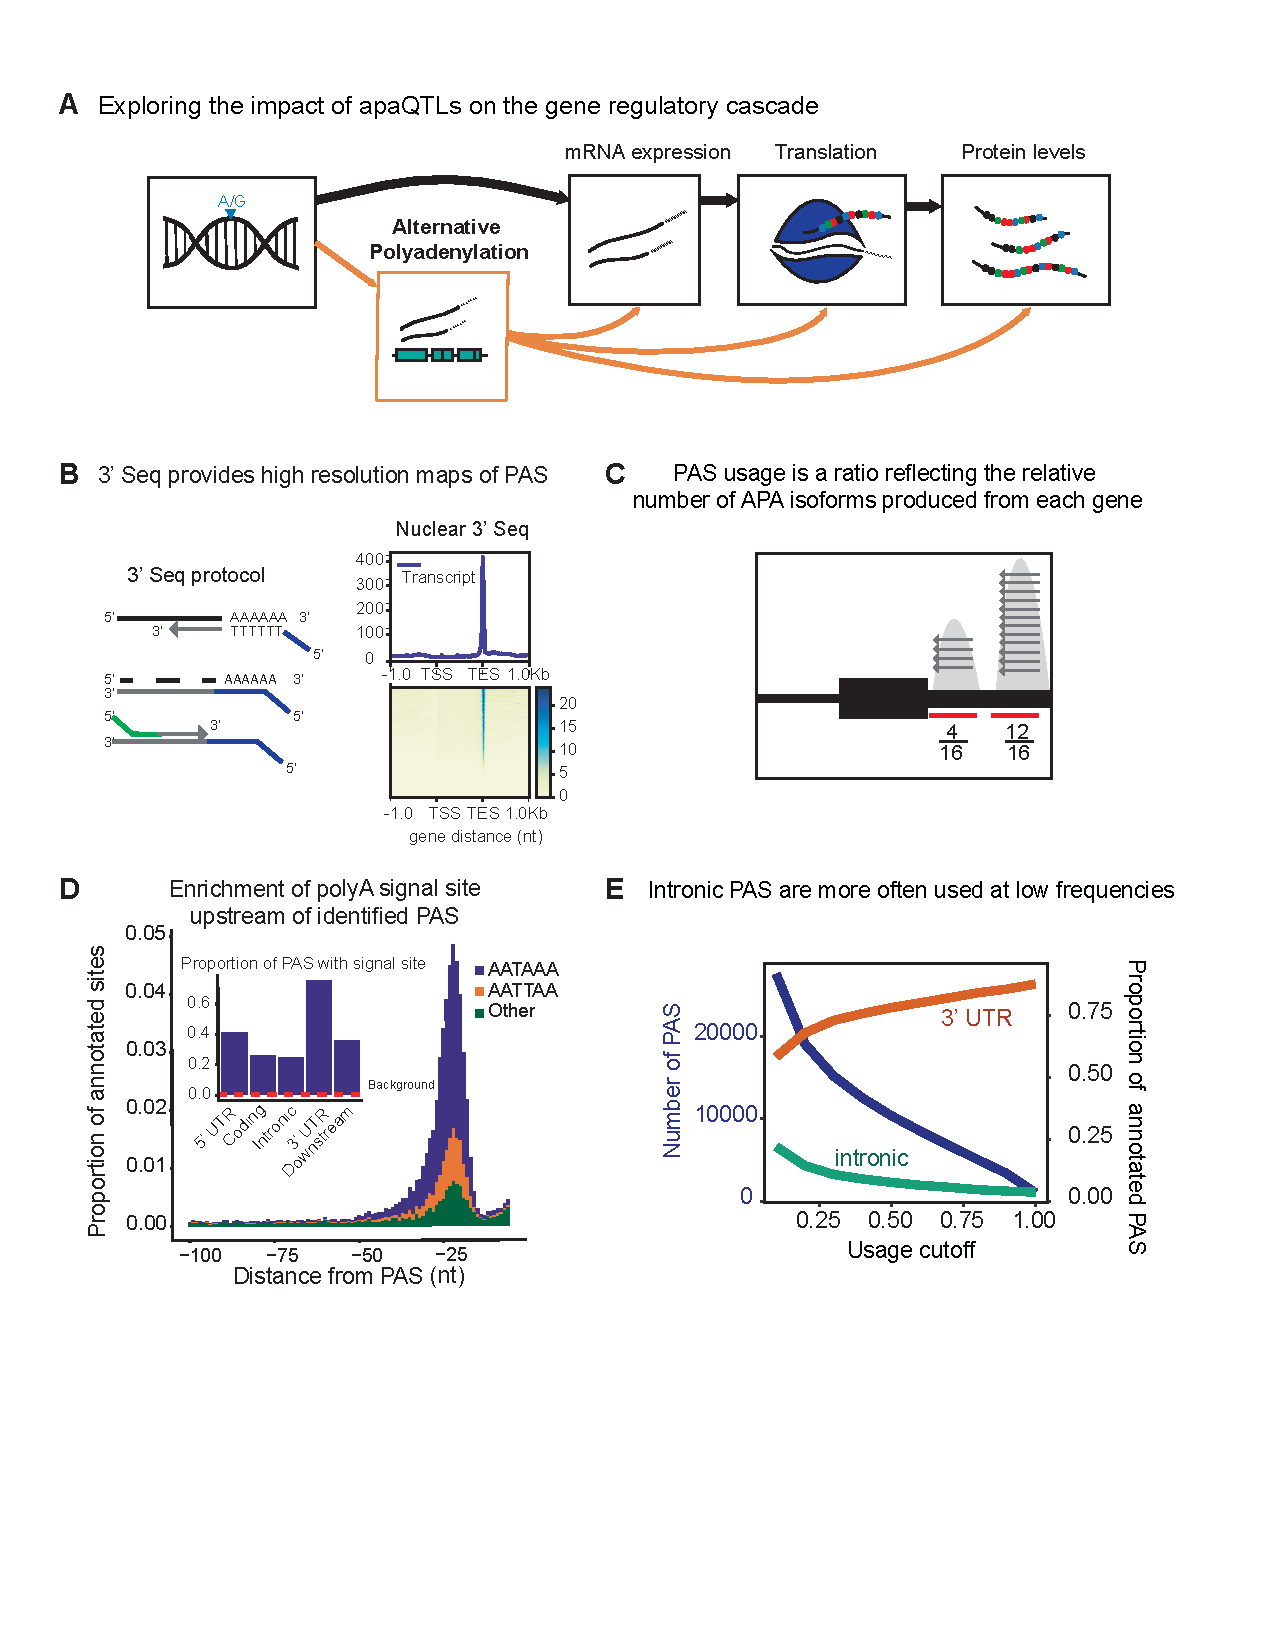
\includegraphics[width=5in]{img/ch02/figure1_fixed.pdf}
\caption[3' Sequencing of nuclei reliably captures alternative polyadenylation]{\small {\bf (A)} Schematic of how genetic variants affect phenotypes by percolating through gene regulatory layers (black arrows). We aimed to understand how genetic variation can mediate gene regulation through alternative polyadenylation (orange arrows). {\bf (B)} {\it (Left)} Schematic of Lexogen Reverse Quant Seq protocol for 3' Sequencing \citep{moll_quantseq_2014} {\it (Right)}Meta gene plot showing read coverage for five 3' Seq libraries collected from nuclei isolated from LCLs. {\bf (C)} Representation for how PAS usage is calculated. Read count for each PAS were divided by the total number of reads at all PAS for the gene. {\bf (D)} {\it (Main)} Stacked density of canonical (AATAAA, AATTAA) and other polyadenylation signal sites (AAAAAA, AAAAAG, AATACA, AATAGA, AATATA, ACTAAA, AGTAAA, CATAAA, GATAAA, TATAA) upstream of identified PAS.} 
\label{fig:3prime4APA}
\end{figure}


% Continues caption on next page. Requires package ccaption.
\begin{figure}[!htb]
\contcaption{(continued) {\it (Inset)} Proportion of PAS in different genomic regions with a polyadenylation signal site 10-50bp upstream of cleavage site. The red dotted line represents the proportion of signal site in random 40bp windows, i.e. the intronic background. {\bf (D)} The blue line represents the number of PAS identified as the stringency of the usage cutoff increases. The orange and green lines represent the proportion of PAS in the 3' UTR and introns, respectively. The proportion of intronic PAS increases as the usage cutoff decreases, implying that a disproportionate number of intronic PAS are used at low frequencies.}
\end{figure}
  
  


\subsection{Genetic loci associated with variation in APA}\label{apa-QTLs}

Having established that APA can contribute to the generation of complex transcript isoforms, we sought to identify genetic loci associated with inter-individual variation in APA. We normalized each PAS usage ratio using LeafCutter  \citep{li_annotation-free_2018} and tested {\it cis}-associations between genetic variants and PAS usage, correcting for batch and the top principal components (Methods, Supplementary Figure \ref{fig:QQplots}, \ref{fig:propPASdAPA}, \ref{fig:PCA}). Using 3' Seq data from the nuclear fraction, we identified 602 nuclear apaQTLs in 479 genes at 10\% FDR. In the total mRNA fraction, we identified 443 apaQTLs in 353 genes at 10\% FDR. For example, individuals with the C/C genotype (rs11032578) show higher usage of an intronic PAS in the {\it ABTB2} gene compared to individuals that are heterozygous C/T or homozygous T/T (Figure \ref{fig:qtlFigure}A). In both fractions, apaQTL lead SNPs are enriched near the PAS they most strongly correlate with and near the 3' ends of gene bodies (Figure \ref{fig:qtlFigure}B, Supplementary Figure \ref{fig:totQTLloc}). The proximity of the apaQTL lead SNPs to PAS may suggest that genetic variants that affect polyadenylation signal motifs drive most of the genetic effects on APA. Although we observed an enrichment of apaQTLs in signal motifs, genetic variants that alter signal motifs are unlikely to explain the majority of apaQTLs (Supplementary Figure \ref{fig:ssDisrupt}).

Our study design provides the unique opportunity to evaluate the likely mechanisms by which genetic variation controls PAS usage. While previous studies have demonstrated that genetic variants can impact PAS usage, it has been difficult to discern whether the variation in PAS usage is primarily driven by genetic effects on cleavage and polyadenylation (Figure \ref{fig:qtlFigure}C, Model 1), or on the mRNA lifecycle (e.g. by impacting miRNA binding sites and decay) (Figure \ref{fig:qtlFigure}C, Model 2). We reasoned that if genetic effects functioned primarily by affecting post-transcriptional regulation such as decay or export, then this effect would be detectable in the total mRNA fraction, but would be smaller or undetectable in the nuclear mRNA fraction (Supplementary file 1). Interestingly, we found that only 97 apaQTLs (of 443 apaQTLs, 21.9\%) identified in the total mRNA fraction were not detected in the nuclear mRNA fractions and these associations are much weaker than shared apaQTLs (Supplementary Figure \ref{fig:totSpeWeak}). We thus suspect that we currently lack statistical power to detect most of these 97 apaQTLs in the nuclear mRNA fraction. To estimate sharing of apaQTLs across the two mRNA fractions, we used Storey's $\pi_0$ statistics and found that the vast majority of apaQTLs identified in the total mRNA fractions were estimated to also affect PAS usage in the nuclear mRNA fraction ($\pi_{1}$=0.87, Supplementary Figure \ref{fig:QTLshare}). In addition, we found that the genetic effect sizes on PAS usage were very similar across the two mRNA fractions ($r^{2}$ = 0.66; $p = 10^{-16}$, Figure \ref{fig:qtlFigure}D, Supplementary Figure \ref{fig:apaQTLcorr}). Altogether these observations show that most genetic variants impact PAS usage by affecting polyadenylation site choice. Supporting this notion, we found weak or no enrichment of apaQTLs in sites bound by RNA binding proteins as identified using eCLIP data from ENCODE (Supplementary file 1).

\begin{figure}
\centering 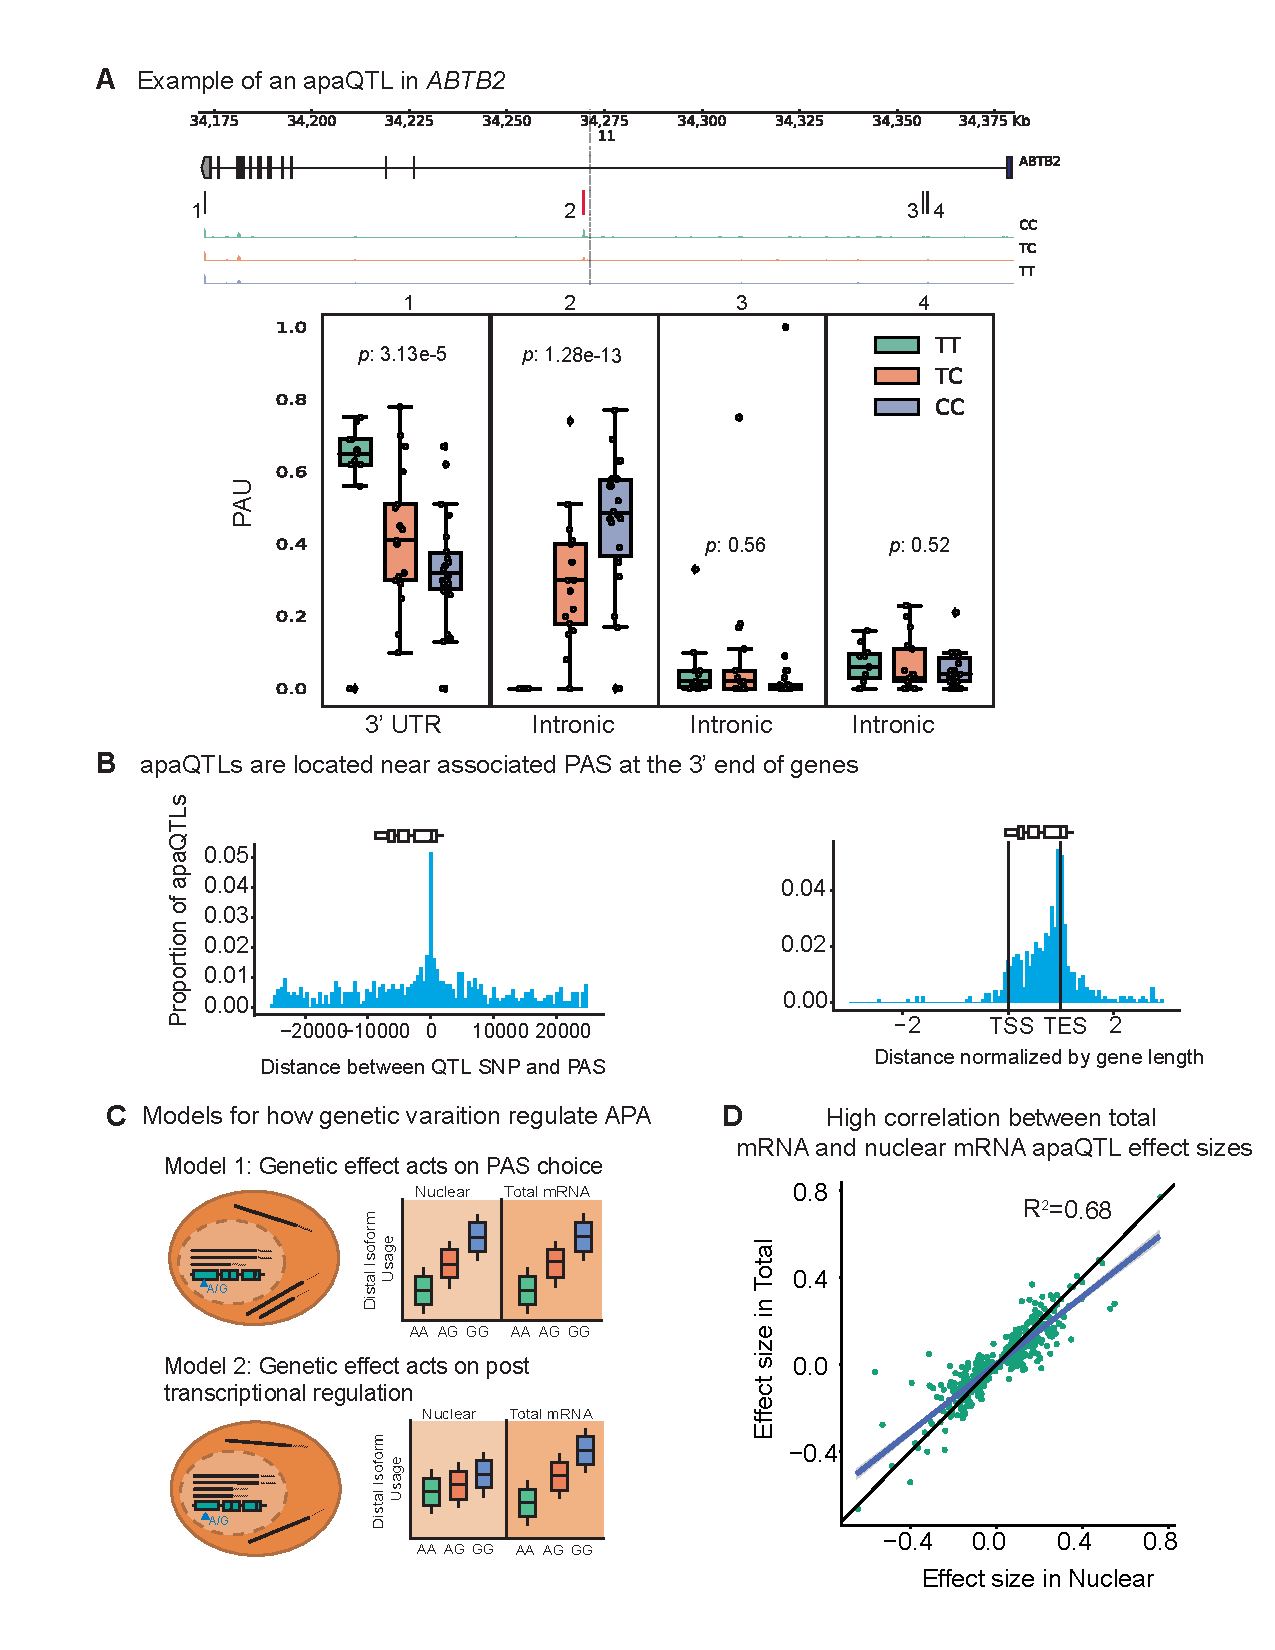
\includegraphics[width=5in]{img/ch02/figure2.pdf}
\caption[Identify genetic variation driving differences in polyadenylation as apaQTLs]{\small {\bf (A)} An apaQTL in the {\it ABTB2} gene impact usage of an intronic PAS. {\it (Top)} Gene track and identified PAS. Each bar represents a potential isoform. The red bar corresponds to the isoform most strongly associated with the apaQTL. The vertical dotted line represents the position of the lead apaQTL SNP. {\it (Bottom)} Boxplot of polyadenylation site usage at each PAS by genotype listed according to the isoform order above. The C allele increases usage of the intronic PAS. {\bf (B)} ({\it Left})  Location of the lead nuclear apaQTL SNPs relative to their corresponding PAS. ({\it Right}) Meta gene plot showing the distribution of apaQTL SNPs in the annotated gene body, where 0 represents the transcription start site and 1 represents the annotated transcription end site.} 
\label{fig:qtlFigure}
\end{figure}


\begin{figure}[!htb]
 \contcaption{(continued) {\bf (C)} Two mechanistic models for how genetic variants can affect PAS usage. ({\it Model 1}) Genetic variation acts directly on PAS choice. In this case, the apaQTL will be identified with similar effect sizes in both nuclear and total mRNA fractions, or smaller effect size in the total mRNA fraction.  ({\it Model 2}) Genetic variation acts through a post transcriptional mechanism. For example, one mRNA isoform is subject to decay. In this case, the apaQTL will be identified only in the total mRNA fraction, or will be identified in the total mRNA fraction with a larger effect size than in the nuclear mRNA fraction.{\bf (D)} Effect sizes of apaQTLs originally identified at 10\% FDR in the nuclear mRNA fraction plotted against the effect sizes ascertained in the total mRNA fraction. Regression line is shown in blue and $y = x$ line is shown in black.}
 \end{figure}
 
 
 

\subsection{Impact of apaQTLs on gene expression levels}\label{apa-QTLs-expression}


While we believe that nearly all genetic variants impact PAS usage by affecting polyadenylation site choice and not isoform-specific decay or export, this model is not incompatible with a model in which genetic variants can sometimes impact expression by affecting APA. For example, a genetic variant might increase the relative production of an isoform that is less stable, in which case total transcript levels would decrease. Therefore, next, we asked whether genetic variants could impact gene expression levels by direct effects on APA. We hypothesized that this mode of genetic regulation may be prevalent, in particular for genes with intronic PAS, because isoforms using intronic PAS are often subject to rapid decay. In this model, the genetic effect changes the relative production of isoforms with different relative stabilities rather than specifically modulating the stability of an isoform e.g. by increasing affinity for microRNA binding in the 3' UTR.

To test this hypothesis, we focused on the set of 602 apaQTLs that we identified in the nuclear mRNA fraction, representing genetic variants that impact PAS choice. Our hypothesis predicts that genetic variants that increase intronic PAS usage should decrease gene expression levels. In line with this prediction, we found a negative correlation between the genetic effect sizes for intronic PAS usage and mRNA expression levels ($p = 8.97 \times 10^{-7}$, Figure \ref{fig:apaandexpression}A, Supplementary Figure \ref{fig:3anooutlier}). Thus, our analysis suggests a widespread mechanism whereby genetic variants decrease mRNA expression levels by increasing choice of isoforms with premature PAS that are subject to rapid decay. Of interest, we found that 13 apaQTLs that were detected only in the nuclear fraction are also eQTLs, which highlights the importance of considering early stages of the mRNA lifecycle to uncover eQTL mechanisms.

To further investigate the contribution of APA to gene expression, we sought to understand the relationship between apaQTLs and a set of eQTLs that we previously classified as those with explained putative mechanisms, explained eQTLs (1164 eQTLs, $\sim$ 60\%) or as unexplained eQTLs (801 eQTLs, $\sim$ 40\%) using data from the same LCLs \citep{li_rna_2016}. The eQTLs with explained putative mechanisms were associated with chromatin-level phenotypes including DNase-I hypersensitivity, histone marks, or DNA methylation, and thus are likely to be mechanistically explained by effects mediated by chromatin-level phenotypes (e.g. enhancer or promoter activity). To test whether apaQTLs might account for unexplained eQTLs, we first asked whether genes with unexplained eQTLs were more likely to also harbor apaQTLs than compared to genes with explained eQTLs. Indeed, we found a significantly higher enrichment of low p-value associations with APA for genes with unexplained eQTLs ($p = 0.01$, Figure \ref{fig:apaandexpression}B, Supplementary Figure \ref{fig:totunexp}) and significantly larger absolute apaQTL effect sizes for unexplained eGene compared to explained eGenes (0.35 vs. 0.3, Wilcoxon Rank sum test, $p=6.6 \times 10^{-4}$). We also found that apaQTLs exhibited an association with chromatin states that was more similar to the unexplained eQTLs than the explained eQTLs. In particular, apaQTLs and unexplained eQTLs were more likely to lie in regions of transcription elongation or are associated with weak transcription, and less likely to lie in enhancers or promoters than explained eQTLs (Supplementary Figure \ref{fig:chromHMM}, Methods). Overall, we estimated that 17.3\% of otherwise unexplained eQTLs were associated with PAS usage (see Methods). For example, an unexplained eQTL for \textit{C10orf88} (rs7904973) colocalizes with an apaQTL associated with increased usage of an intronic PAS (Figure \ref{fig:apaandexpression}C). More generally, we found that eQTLs and apaQTLs colocalize for the majority of genes that had both (Methods, Supplementary file 1). These observation thus highlights APA as one important mechanism by which genetic variation impacts gene expression independent from enhancers and promoters. 
  

\begin{figure}
\centering 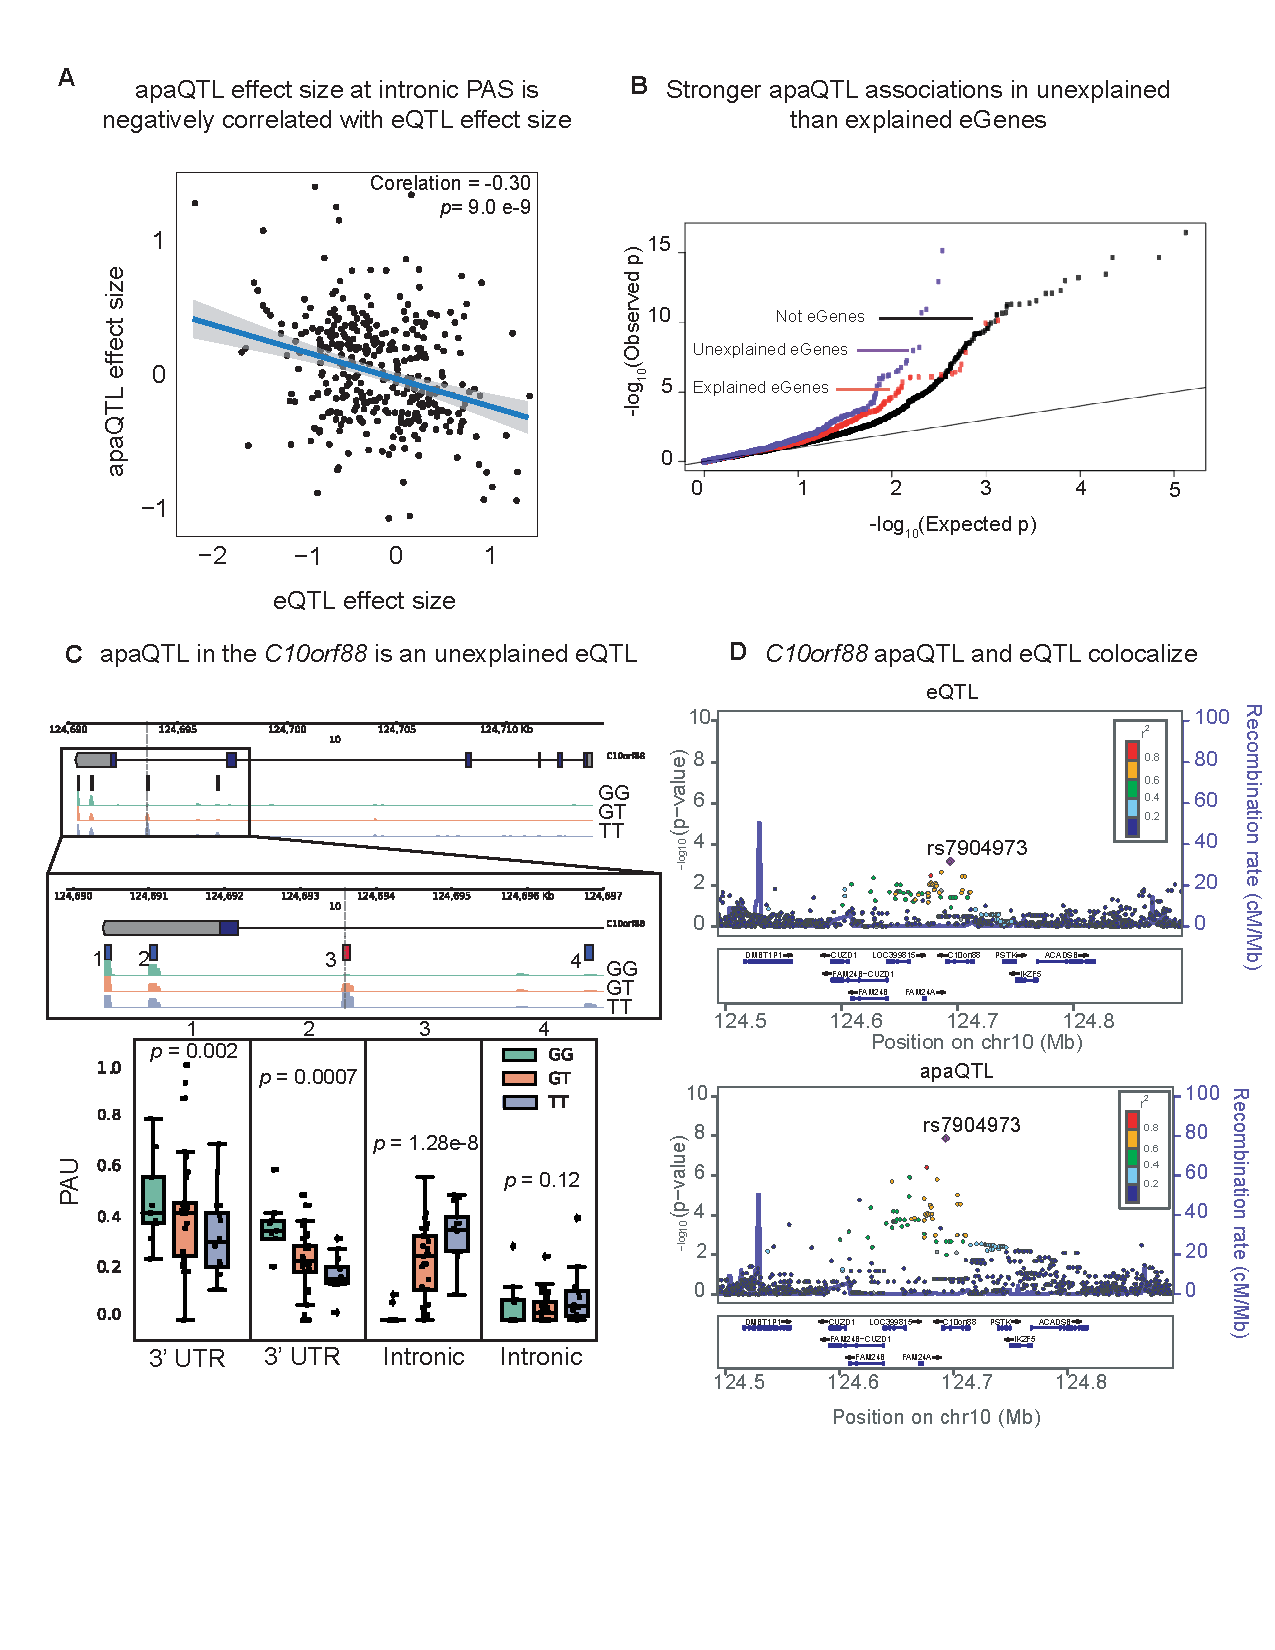
\includegraphics[width=5in]{img/ch02/figure3.pdf}
\caption[apaQTLs provide mechanistic evidence eQTLs ]{\small {\bf (A)} Scatter plot of intronic apaQTL effect sizes plotted against their eQTL effect sizes shows negative correlation. {\bf (B)} Quantile-quantile (Q-Q) plot for apaQTLs shows that apaQTLs are more highly enriched in unexplained eGenes (purple dots) compared to explained eGenes (red dots). {\bf (C)} Example of an apaQTL that is also an unexplained eQTL for {\it C10orf88}. {\it (Top)} Gene track and identified PAS in the {\it C10orf88} gene. The red bar corresponds to the isoform most strongly associated with the apaQTL. The vertical dotted line represents the position of the strongest apaQTL SNP. {\it (Middle)} Zoomed version of track represented above. {\it (Bottom)} Boxplot of polyadenylation site usage at each PAS by genotype listed according to isoform order above. {\bf (D)} {\it (Top)} LocusZoom plot for eQTL associations for the {\it C10orf88} gene. ({\it Bottom)} Locus zoom plot for apaQTL associations. Interestingly, the lead apaQTL and eQTL SNP, rs7904973, has been linked to increased LDL cholesterol through GWAS \cite{klarin_genetics_2018}.}
\label{fig:apaandexpression}
\end{figure}


\subsection{APA mediates gene regulation independently of mRNA expression levels}\label{APA-independent-expression}

Previous joint analyses of molecular QTLs suggested that functional genetic variants tend to affect gene regulation in a simple and straightforward manner: first impacting chromatin activity, then mRNA expression, and finally protein expression \citep{li_rna_2016, battle_genomic_2015}. However, because isoforms with different 3' UTRs have been shown to vary in terms of their translation efficiency, we hypothesized that apaQTLs can impact ribosome occupancy and protein expression levels without affecting mRNA expression levels \citep{floor_tunable_2016-1}. To test this possibility, we asked whether apaQTLs are enriched among genes without a known eQTL, but that are associated with a ribosome occupancy QTL (riboQTL) or a protein expression QTL (pQTL). Indeed, we found that apaQTLs are enriched among genes with a ribosome QTL (rGenes; Wilcoxon rank sum test, $p=0.01$) and genes with a pQTL (pGenes; Wilcoxon rank sum test, $p = 0.0006$) compared to genes with no molecular association (Figure \ref{fig:expInd}A, Supplementary Figure \ref{fig:totpgene}) \cite{li_rna_2016, battle_genomic_2015}. In addition, we observed a small but significant positive correlation between individual variance in APA usage and ribosome occupancy  (correlation = 0.15, $p <2.2\times10^{-16}$, Supplementary file 1), supporting a model in which APA impacts translation efficiency.

In total, we found 24 apaQTLs that affect protein expression, but not mRNA expression (Table \ref{tab:ch02-s1}). Of these, five apaQTLs were significantly associated with ribosome occupancy (Table \ref{tab:ch02-s1}). This finding is particularly noteworthy because nearly all genetic effects on ribosome occupancy have been proposed to be mediated by effects on mRNA expression \citep{battle_genomic_2015}. Yet, here we provide direct evidence that APA can mediate genetic effects on ribosome occupancy without affecting mRNA expression levels. For example, the apaQTL in the {\it EIF2A} gene that is associated with a switched usage of two 3' UTR PAS, colocalizes with a pQTL and a ribosome occupancy QTL (Figure \ref{fig:expInd}B, Supplementary Figure \ref{fig:locuszoom}), but is not associated with {\it EIF2A} mRNA levels (Figure \ref{fig:expInd}B). Interestingly, the QTL in {\it EIF2A} affects usage of two PAS in the same 3' UTR implying that the protein sequence encoded by the two isoforms are identical. Thus, the regulatory associations uncovered at {\it EIF2A} cannot simply be explained by differences in protein isoform stability. Moreover, while differences in 3' UTR are often assumed to play a regulatory function by influencing decay \citep{mayr_regulation_2017}, mechanisms involving RNA decay cannot be operational in this case because steady-state mRNA expression is unchanged. Instead, differences between the two isoforms may reflect differential binding of factors that impact translation \citep{yamashita_translational_2017}, or differential rates of translation re-initiation at the end of a translation cycle \citep{rogers_ribosome_2017}. 

We identified 19 pQTLs that were associated with APA but not steady-state gene expression or ribosome occupancy levels. Two previous studies also reported the discovery of pQTLs that were not eQTLs \citep{battle_genomic_2015, chick_defining_2016}. In both studies, the authors proposed that some genetic effects on protein expression levels were mediated by changes in the protein sequence or by changes in the expression level of interacting proteins, which would manifest post-translationally. Our finding reveals yet another mode of genetic regulation of protein expression level by APA (e.g. by affecting recruitment of interacting proteins). Thus, these findings provide clear evidence that APA can affect protein expression levels without affecting gene expression levels. Altogether, our findings suggest complex modes of gene regulation independent of mRNA expression driven by variation in APA.


\begin{figure}
\centering
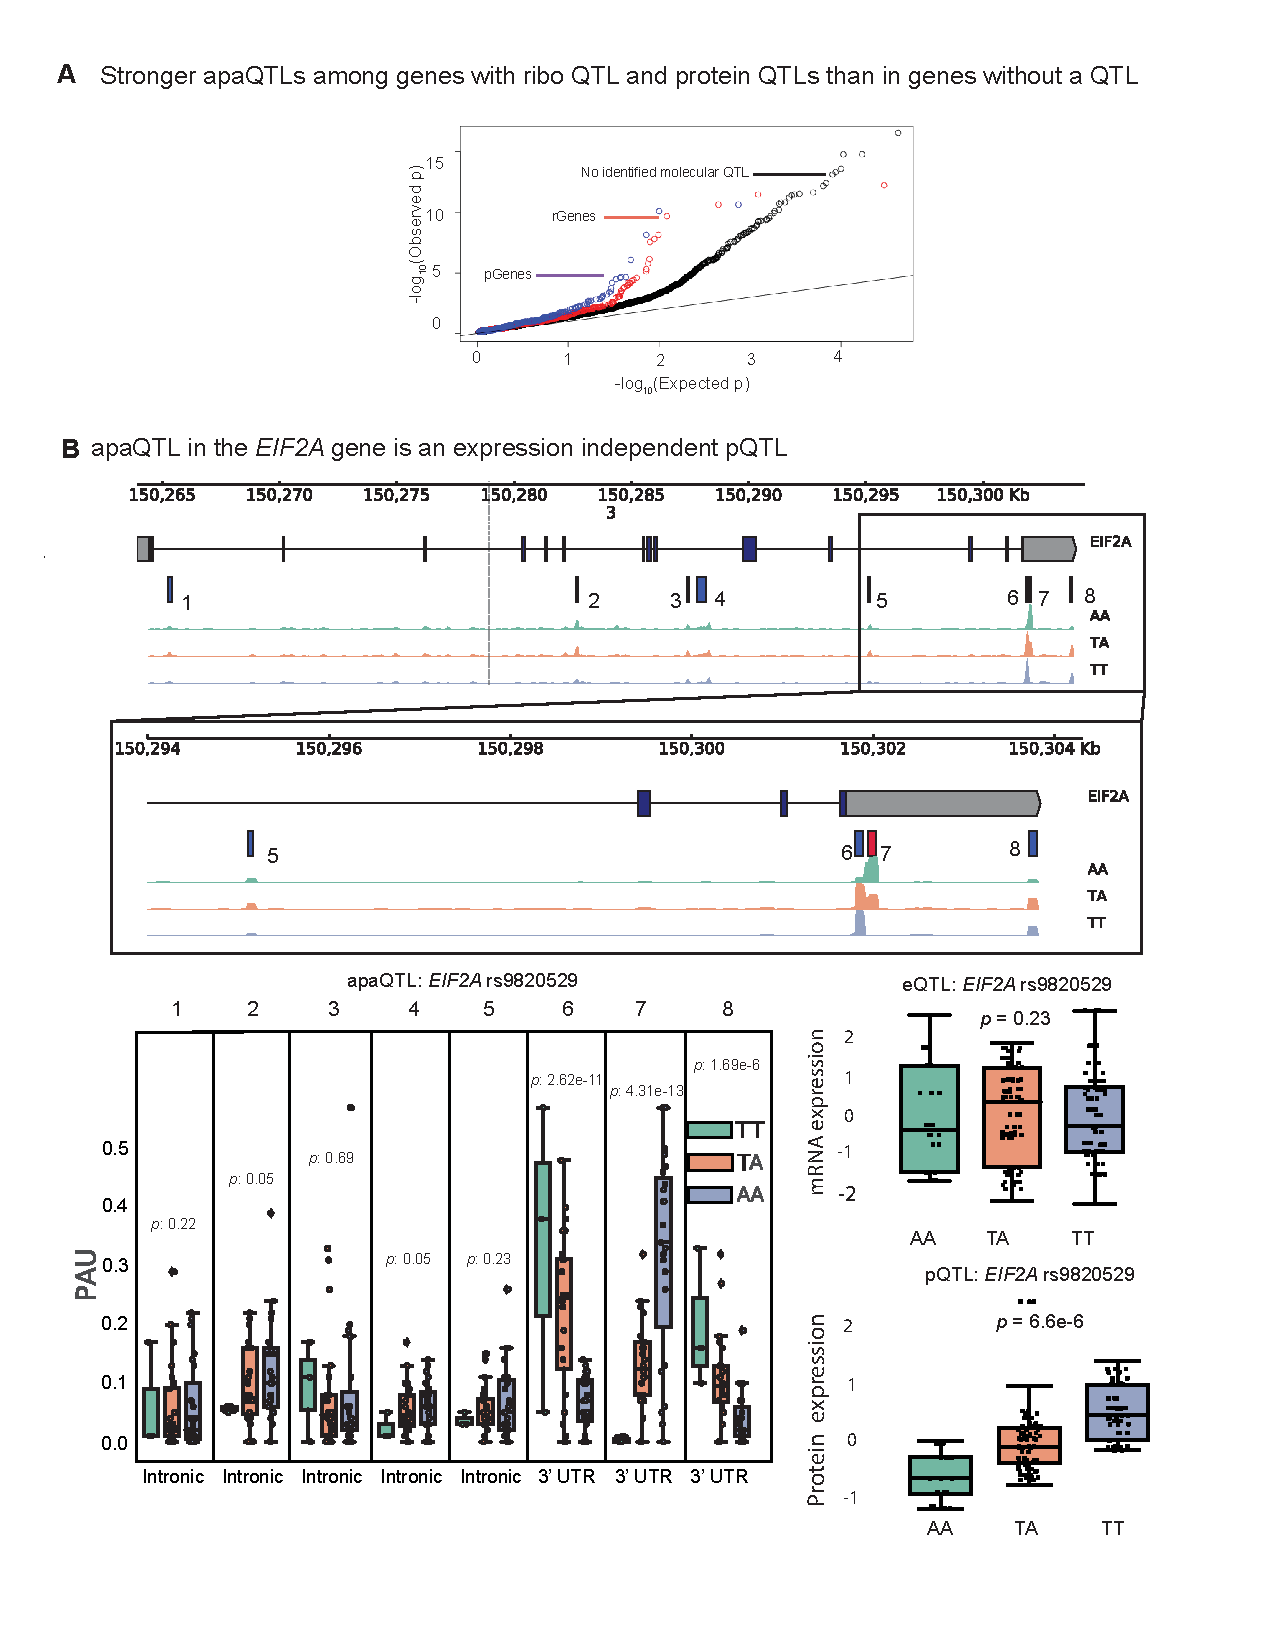
\includegraphics[width=5in]{img/ch02/figure4.pdf}
\caption[apaQTLs explain expression independent rQTLs and pQTLs] {\small {\bf (A)} Quantile-quantile (Q-Q) plot for apaQTLs separated by genes in previously detected rQTLS (red) and pQTLs (purple) that are not eQTLs. Black points are apaQTL genes with no pQTL, rQTL, or eQTL. {\bf (B)}{\it (Top)} Gene track and identified PAS in the {\it EIF2A} gene. The red bar corresponds to the isoform most strongly associated with the apaQTL. The vertical dotted line represents the position of the strongest apaQTL SNP. {\it (Middle)} Zoomed version of track represented above. {\it (Bottom Left)} Boxplot of polyadenylation site usage at each PAS by genotype listed according to isoform order above.  {\it (Top Right)} Boxplot showing normalized mRNA expression for {\it EIF2A} by genotype at the apaQTL SNP (rs9820529).   {\it (Bottom Right)} Boxplot showing normalized protein expression for {\it EIF2A} by genotype at the apaQTL SNP (rs9820529).}
\label{fig:expInd}
\end{figure}


\subsection{APA mediates genetic effects on complex traits}\label{APA-traits}

Genetic variation may impact disease risk through APA. We asked whether common variants in the regions around PAS, i.e. regions enriched for apaQTLs, are enriched in disease heritability. Using LDscore regression to estimate the heritability enrichment of 35 traits in 1kb regions centered around PAS, we found that 14 of the tested traits were significantly enriched (\ref{fig:ldregress}). Of note, genetic variation around PAS was estimated to tag 15.35\% of the SNP heritability for rheumatoid arthritis (7.88 fold enrichment, $p = 0.0025$). We further asked whether we could identify specific apaQTLs associated with phenotype. Indeed, 19.3\% of apaQTLs (including SNPs in LD with $r^{2} > 0.9$) are significantly associated with at least one trait in the UCSC GWAS catalog (Methods) \citep{kent_human_2002}. For example, an apaQTL that colocalizes with the eQTLs in the C10orf88 gene (rs7904973) has been associated with increased LDL cholesterol \citep{klarin_genetics_2018}, suggesting that eQTLs mediated by APA can impact organismal phenotype. Taken together, we propose that APA is a complex regulatory mechanism relevant to our understanding of how genetic variation can affect disease. Thus, comprehensive maps of apaQTLs can enhance our ability to interpret GWAS loci, particularly when the implicated variants are not eQTLs \citep{joehanes_integrated_2017, lee_widespread_2018}. For example, an apaQTL in the {\it ELL2} gene (rs56219066) is correlated with increased usage of an intronic PAS and is associated with risk for multiple myeloma \citep{swaminathan_variants_2015}. Interestingly, multiple myeloma is among the cancer types in which widespread dysregulation of intronic APA has been documented previously \citep{singh_widespread_2018, lee_widespread_2018}.



\section{Discussion}\label{ch02-discussion}

Obtaining a comprehensive understanding of the mechanisms that affect gene regulation is crucial for the functional interpretation of noncoding genetic variation. Yet, existing studies that examine the role of genetic variation on APA are generally characterized by two important shortcomings. Firstly, the study of inter-individual variation in PAS usage have been mostly restricted to APA in the 3' UTRs \citep{li_genetic_2019, yoon_genetics_2012, yang_snp2apa_2019}, leaving genetic variants that impact PAS usage in other regions, e.g. intronic PAS, understudied. Secondly, nearly all existing studies use standard RNA-seq to estimate PAS usage, which not only limits the accuracy of usage quantification, but also makes it difficult to disentangle the contribution of co-transcriptional mechanisms to APA regulation from post-transcriptional mechanisms such as isoform-specific decay. In this study, we overcome these shortcomings by applying 3' Seq to total and nuclear mRNA fractions separately to directly measure PAS usage including that of PAS in intronic regions. 

It is worthwhile to note here that despite the many advantages of using 3' Seq to identify and quantity APA isoforms, 3' Seq experiments are known to be susceptible to mispriming, which occurs when polydT primers designed to recognize the polyA-tail of transcripts anneal to adenosine stretches within a transcript, thus introducing false positive polyadenylation sites. While we used stringent criteria to reduce the effect of mispriming, we found that a small proportion of PAS used in this study may be the result of mispriming. In particular, we found an enrichment of adenosine nucleotides at a subset of intronic PAS which were discovered in our study and not previously annotated, suggesting that 10--20\%{} of unannotated intronic PAS may be false positives (Supplementary file 1). To ensure that these false positive PAS do not affect the validity of our analyses, we performed the main analyses presented in this study after removing unannotated intronic PAS and found that our conclusion were robust to the small number of potential false positive intronic PAS (Supplementary file 1) \citep{wang_polya_db_2018}. 


By collecting data from both total and nuclear mRNA factions, we were able to study the effects of genetic variation on polyadenylation at multiple stages of the mRNA lifecycle, and to distinguish putative regulatory mechanisms by noting the stages at which the genetic effects on APA were observed.  For example, genetic variants can impact steady-state isoform ratio either co-transcriptionally by affecting PAS choice during transcription (Figure \ref{fig:qtlFigure}C top), or  post-transcriptionally by affecting binding of miRNAs or RNA-binding proteins and consequently isoform decay (Figure \ref{fig:qtlFigure}C bottom). We found that the vast majority of genetic variants that affect PAS usage ratio in total mRNA fraction, were also found to have similar effect sizes on PAS usage ratio in the nucleus. This observation implies that inter-individual variation in steady-state APA levels can generally be explained by variation in co-transcriptional mRNA processing, or mRNA processing that occur soon after transcription. 

There are several co-transcriptional mechanisms that may result in variation in PAS usage. For example, previous reports have suggested that variation in the polyadenylation signal site may cause variation in PAS usage. While we found that this was the case for a small number of examples, disruption of canonical signal motifs does not appear to be a major mechanism for generating apaQTLs, an observation that is also supported by a recent study on APA in GTEx data (Supplementary Figure \ref{fig:ssDisrupt}) \citep{li_genetic_2019}. Other possible co-transcriptional mechanisms involved in PAS choice include competition between the spliceosome and polyadenylation factors for example mediated by the spliceosomal RNA U1 \citep{oh_u1_2017}, and RNAP II pausing \citep{fusby_coordination_2016}. Indeed, recent studies have reported that sequence and chromatin context can pause or slow down RNAP II elongation across the gene body \citep{mayer_native_2015}, suggesting that variation in RNAPII pausing may impact PAS choice \citep{fusby_coordination_2016}. For example, in Drosophila melanogaster, paused RNAPII promotes the recruitment of ELAV on the pre-mRNA, which prevents usage of a proximal PAS \citep{oktaba_elav_2015}. In addition, Liu et al. observed a tissue-specific shift toward usage of proximal PAS sites in Drosophila melanogaster mutant for a slow elongation form of RNAPII \citep{liu_transcription_2017}. These findings further suggest that variants affecting RNAPII elongation rate could underlie the genetic effects on PAS usage we detected in this study. 

Although our data suggest that apaQTLs do not generally impact rates of mRNA decay, e.g. by affecting miRNA or RBP binding motifs, we found clear evidence that apaQTLs may promote polyadenylation site choices that result in the production of isoforms with different rates of decay. For example, we observed that genetic variants that increase the usage of isoforms ending at intronic PAS tend to be associated with lower levels of gene expression. This observation is consistent with reports that isoforms with premature polyadenylation are often substrates for nonsense mediated decay or nonstop decay \citep{tian_alternative_2017, vasudevan_non-stop_2002}. More generally, our results suggest that apaQTLs can affect gene expression levels post-transcriptionally by impacting the production of isoforms with varying levels of stability. Importantly, our study highlights APA as an eQTL mechanism independent of promoters and enhancers. 


While the effect of genetic variants on gene regulation is generally assumed to move linearly from chromatin, to mRNA, to protein level, our study reveals several complex modes of genetic regulation for both gene expression and protein expression levels by APA. Although we were unable to study the genome-wide effects of APA on protein expression owing to a scarcity of protein-level data, we identified several apaQTLs that affect protein, but not gene expression levels. These results strongly suggest that APA can affect protein expression levels without affecting gene expression levels, because our power to detect genetic effects on gene expression levels far exceeds that to detect genetic effects on protein expression levels. Furthermore, some of these pQTLs were associated with ribosomal occupancy and some were not, which implies multiple pathways by which genetic variants can impact protein expression levels through APA.

In conclusion, there are many pathways through which genetic variants can impact gene regulation and, consequently, organismal phenotypes. While many studies have demonstrated the importance of gene expression regulation through promoters or enhancers, very few studies have focused on co- or post-transcriptional gene regulation. Our study shows that co- and post-transcriptional processes such as APA can mediate the effects of a substantial number of genetic variants on mRNA expression levels, protein expression levels, and risk for complex diseases.


\section{Methods}\label{ch02-methods}

\subsection{Cell Culture}\label{ch02-cell-culture}

We cultured 54 Epstein-Barr virus transformed LCLs under identical conditions at 37 C and 5\% CO2. These LCLs were derived from Yoruba individuals originally collected as part of the HapMap project \cite{international_hapmap_consortium_haplotype_2005}.The sampleIDs and Research Resource Identifiers (RRIDs) can be found in online version of paper (see chapter citation). Details for each cell line are found in Supplementary file 3. We grew cells in a glutamine depleted RPMI [RPMI 1640 1X from Corning (15-040-CM)], completed with 15\% FBS, 2mM GlutaMAX (from gibco (35050-061), 100 IU/ml Penicillin, and 100 ug/ml Streptomycin. After passaging them 3 times the lines were maintained at a concentration of $1\times10^{6}$ cells per mL. In preparation for extraction, we allowed the cells to grow until a concentration of $1\times10^{6}$ cells per mL was reached and then proceeded to extraction. \

\subsection{Collection and RNA extraction}\label{Collection-and-RNA-extraction}

We collected 30 million cells from each line and divided them into two 15 million cell aliquots. We spun the cells down at 500 RPM at 4C for 2 min, and then washed the pellets with phosphate-buffered saline (PBS) and spun down again. After this we aspirated the PBS, leaving the cell pellet. All washing steps occurred on ice or in cooled centrifuges. At this point every cell line had two separate pellets each from an input of 15 million cells. From each line we took one of these pellets for nuclear isolation. We then carried out nuclear isolation using the nuclear isolation steps outlined by \citep{mayer_genome-wide_2016}. Once we washed and spun down the pellets in the nuclei wash buffer, we resuspended them in 700 ul of the QIAzol lysis reagent (Qiagen). We extracted both RNA cell pellets from the same line in the same batch using the miRNeasy kit (Qiagen) according to manufacture instructions, including the DNase step to remove potentially contaminated genomic DNA. Details for the collection such as cell viability and cell concentration at time of collection are found in Table \ref{tab:ch02-s2}. We checked the quality of the collected RNA using a nanodrop. RNA concentrations and absorbance levels from the collection are in Table \ref{tab:ch02-s2}.

In order to verify fraction separation, we completed the Mayer and Churchman protocol to isolate chromatin and collected cell lysates for each step in the fractionation \citep{mayer_genome-wide_2016}. We performed western blots against both GAPDH (GAPDH antibody (6C5) Life Technologies AM4300) and the Carboxyl Terminal Domain of Pol-II (CTD) (Pol II CTD Ser5-P antibody, Active Motif, 61085). We ran each lysate on Mini-protean TGX precast gels (bioRad 456-1093) after digesting any remaining DNA molecules from the nuclear isolate with benzonase nuclease. We used Goat anti-Mouse IgG (H+L) (Invitrogen 32430) as a secondary antibody for the GAPDH antibody and Goat anti-Rat IgG (H +L) (Invitrogen 31470) as a secondary antibody for the CTD antibody. We diluted all antibodies in a 1:1000 dilution with blocking solution made from dry milk (LabScientific Lot 1267N Cat M0841). We show GAPDH isolated in the cytoplasm and CTD to the chromatin fraction (Supplementary Figure \ref{fig:western}).


\subsection{3' Sequencing library generation}\label{three-Sequencing-library-generation}

We generated 108 single-end RNA 3'sequencing libraries from the total and nuclear RNA extract using the QuantSeq 3 ' mRNA-Seq Library Prep Kit \citep{moll_quantseq_2014} as directed by the manufacturer. We used 5ng of each sample as input. We submitted the libraries for sequencing on the Illumina NextSeq5000 at the University of Chicago Genomics Core facility using single end 50bp sequencing. 

\subsection{3' Sequencing data processing}\label{three-Sequencing data processing}

We mapped 3'  Seq reads to hg19 \citep{church_modernizing_2011} using STAR RNA-seq aligner \citep{dobin_star_2013} using default settings with the WASP mode to filter out reads mapping with allelic bias \citep{van_de_geijn_wasp_2015}. Similar to previously published 3'  Seq methods, we accounted for internal priming by filtering reads preceded by 6 Ts in a row or 7 of 10 Ts in the 10 bases directly upstream of the mapping position in the reference genome \citep{tian_large-scale_2005, sheppard_accurate_2013, beaudoing_patterns_2000}. We verified the individual identity of all bam files using VerifyBamID \citep{jun_detecting_2012}. Due to low confidence in the identity of 2 individuals, they were removed from all analysis. Raw read and mapped read statistics after accounting for internal priming can be found in Table \ref{tab:ch02-s2} (Supplementary Figure \ref{fig:nucMap}, \ref{fig:TotalMap} \ref{fig:NucMapCount}, \ref{fig:TotMapCount}).

\subsection{Identification and characterization of PAS}\label{Identification-and-characerization-of-PAS}

We merged all mapped reads and called peaks using an inclusive method, identifying all regions of the genome with non-zero read counts in 90\% percent of libraries and an average read count of greater than 2 counts. This resulted in 138,181 peaks. We assigned each of these peaks to a genic location according to NCBI Refseq annotations for 5' UTRS, 3' UTRs, exons, introns, and regions 5kb downstream of annotated genes downloaded from the UCSC table browser \citep{kent_human_2002}. When a region mapped to multiple genes we used a hierarchical model, similar to the method used by Lin et al. \citep{lin_-depth_2012} to assign the peak to a gene annotations. Our method prioritizes annotations in the following order: 3' UTRs, 5kb downstream of genes, exons, 5'  UTRs, and introns. To further verify absence of PAS detected as a result of internal priming we removed PAS with 6A's or 70\% As in the 15 basepairs downstream of the site. We next utilized a gene level noise filter to account for non-uniform read coverage across the genome. We created a usage score for each PAS based on of the number of reads mapping to the PAS over the number of reads mapping to any PAS associated with the same gene. We filtered out peaks with a mean usage of less than 5\% in both the total and nuclear libraries. After this filter, we were left with 35,032 PAS in the total mRNA fraction and 39,164 PAS in the nuclear fraction. The merged set with PAS from both fractions used for PAS QC is available on GEO and has 41,810 PAS. We compared our set of PAS to the human PolyADB release 3.2 annotation \citep{wang_polya_db_2018}(Supplementary Figure  \ref{fig:compAnno}). We explored the relationship between number of PAS detected and gene expression using TPM estimates from YRI LCLs after removing very lowly expressed genes (less than 1 TPM) \citep{lappalainen_transcriptome_2013}. We calculated the 5' splice site strength using the MaxEntScore tool, for each of the introns in our annotation \citep{yeo_maximum_2004}. We binned the introns by decile according to the scores and evaluated the distribution of the introns containing PAS. We also used the scores for the introns containing PAS to investigate the relationship between PAS usage and 5' splice site strength.

\subsection{PAS Signal site enrichment and locations}\label{PAS-Signal-site-enrichment-and-locations}

We used the Homer findMotifsGenome.pl script  with the -size -300,100  option to identify binding motifs in the 50bp upstream of each PAS \citep{heinz_simple_2010}. As a background, we used genome shuffle to randomly chose the same number of 50bp regions. To explore the location of the signal site relative to the PAS (most 3' end of each identified peak), we determined the relative position of previously described potential signal sites to this position \citep{beaudoing_patterns_2000}. We then extended each PAS 100bp upstream and identified the starting position of each of the 12 PAS signal site variations identified by Beaudoing et al. without allowing for sequence mismatch  \citep{beaudoing_patterns_2000}. 


\subsection{Differential Isoform analysis}\label{Differential-Isoform-analysis}

We mapped 3' Seq reads to all PAS peaks with mean coverage of 5\% in the total or nuclear fraction libraries. This results in 41,813 annotated sites. We assigned reads to PAS using the featureCounts tool with the -O flag to assign reads to all overlapping features \citep{liao_featurecounts_2014}. We ran the leafcutter\_ds.R script on chromosomes 1-22 separately using the cellular fraction label as the sample group identifier \citep{li_annotation-free_2018}.  This analysis tests 9790 genes and resulted in 8227 genes with significant (FDR 10\%) isoform level differences between the total and nuclear cellular fraction. We called differentially used PAS as sites with a $\Delta$ polyadenylation site usage ($\Delta$ PAU) greater than 0.2 or less than -0.2. In our analysis a positive $\Delta$PAU corresponds to increase usage in the total cellular fraction while a negative $\Delta$ PAU corresponds to increased usage in the nuclear fraction. 

\subsection{apaQTL calling in both fractions}\label{apaQTL-calling-in-both-fractions}

We used the leafcutter prepare\_phenotype\_table.py script with default settings to normalize the PAS usage ratios across individuals within each fraction. This method also outputs the top principal components (PCs) of the data to use as covariates. We plotted the proportion of variation explained by each PC in order to identify the number of PCs to include in the analysis (Figure 2.13). We included the top 4 PCs as well as the library preparation batch as the covariates. We plotted the proportion of variance explained by a number of cofactors in each of the top 10 PCs. (Supplementary Figure \ref{fig:PCA}) The top four PCs correlate most strongly with the cell count at collection (Supplementary Figure  \ref{fig:PCA}). We used the same genotypes from Li et al. 2016\citep{li_rna_2016}, available at http://eqtl.uchicago.edu/jointLCL/genotypesYRI.gen.txt.gz \citep{li_rna_2016}. We removed individual NA19092 due to lack of genotype information in this file, bringing our sample size to 51 individuals for this part of the analysis. Only SNPs with a MAF $>$ 5\% in our sample were included. We used FastQTL to map apaQTLs in cis (25kb on either side) with 1000 permutations to select the top SNP-PAS association \citep{ongen_fast_2016}. We called apaQTLs in each fraction as variants passing 10\% FDR (Benjamini-Hockberg) after permutations. In order to plot interpretable effect sizes for each association we computed nominal PAS:SNP associations for the pre-normalized PAS ratios.


\subsection{Association of apaQTLs with chromatin states}\label{Association-of-apaQTLs-with-chromatin-state}

We downloaded the GM12878 chromatin HMM annotations for Hg19 from the UCSC table browser \citep{kent_human_2002}. We overlapped the eQTLs identified and published in Li et al. 2016\citep{li_rna_2016} as well as the total and nuclear fraction apaQTLs with these categories. We calculated 95\% confidence intervals for each measurement by sampling the number of QTLs in the set with replacement 1000 times (Supplementary Figure  \ref{fig:chromHMM}). 


\subsection{apaQTL overlap with eQTLs}\label{apaQTL-overlap-with-eQTLs}
We obtained the set of explained and unexplained eQTLs from Li et al. 2016 \citep{li_rna_2016}. In order to test whether genes with an unexplained eQTL are more likely to be explained by variation in APA, we separated the permuted apaQTL association (top snp per PAS) into three categories: unexplained eGene, explained eGene, non eGenes. We tested for significant enrichment of apaQTLs in each category using one-sided Wilcoxon rank sum tests. In order to test if each explained and unexplained eQTLs described in Li et al. 2016\citep{li_rna_2016} overlaps with an apaQTL, we extracted the nominal associations for each eQTL gene-SNP pair from the apaQTL data in both fractions. In order to account for multiple PAS associations for each pair, we selected the most significant p-value and used a Bonferroni correction to account for the number of PAS tested in the gene. We consider an eQTL as explained by an apaQTL if the corrected p-value is less than 0.05 but report the values for a range of cutoffs in Supplementary Figure \ref{fig:popExp}. We performed colocalization with the R coloc package \citep{wallace_statistical_2012}. The Bayes Factor colocalization method reports Bayes Factors for 4 alternative hypotheses. PP0: No association with either trait, PP1: No association with trait 1, PP2: No association with trait 2, PP3: Association with trait 1 and trait 2, two independent SNPs, and PP4: Association with trait 1 and trait 2, one shared SNP. If causal SNPs for an apaQTL and an eQTL is the same SNP, then PP4 is expected to be large (greater than 0.5). We accounted for incomplete power using the method described in Ongen et al. (Supplementary file 1) \citep{ongen_estimating_2017}.


\subsection{apaQTLs overlap with ribosome specific and protein specific QTLs}\label{apaQTLs-ribosome-specific-protein-specific-QTLs}
The list of protein specific QTL genes can be found in the supplementary information from Battle et al. 2015\citep{battle_genomic_2015}. In order to show that genes with an eQTL and protein specific QTLs are likely to be associated with APA, we separated the permuted apaQTL association (top snp per PAS) into three categories: eGene, pGene, or neither pGene nor eGene. We performed the same analysis with rGenes, eGenes, and neither rGenes nor eGenes. We tested for significant enrichment with one sided Wilcoxon rank sum tests (Figure \ref{fig:expInd}A, Supplementary Figure \ref{fig:totpgene}). 


\subsection{Identification of molecular QTL associations}\label{Identification-molecular-QTL-associations}
We sought to test if SNPs identified as apaQTLs are significantly associated with other molecular phenotypes previously tested in the same panel of LCLs. We tested for associations between the genotypes used in this study and each gene for each phenotype with fastqtl using the top 5 PCs calculated in Li et al. 2016 as covariates \citep{li_rna_2016}. We used normalized RNA expression, RiboSeq values, and protein levels, published in Li et al. 2016 \citep{li_rna_2016}. 


\subsection{PAS heritability estimates and apaQTL overlap with GWAS Catalog}\label{PAS-heritability-estimates-GWAS-Catalog}
We downloaded GWAS summary statistics from both Astle et al. and Okada et al. \citep{astle_allelic_2016, okada_genetics_2014} We augmented our PAS sites by 500bp on either side and ran LD score regression using methods described in Bulik-Sullivan et al. \citep{bulik-sullivan_ld_2015} We downloaded the CRCh37hg19 GWAS catalog for UCSC table browser \citep{kent_human_2002}. We identified SNPs in LD with the nuclear apaQTLs using the LDproxy tool from LDlink with YRI as the population \citep{machiela_ldlink_2015}. We filtered all results to SNPs with an r2 greater than 0.9. We overlapped the full set with the GWAS catalog using pybedtools. 



\subsection{Data and code
availability}\label{ch02-data-and-code-availability}

Fastq files and PAS annotations are available at GEO under accession GSE138197 \url{https://www.ncbi.nlm.nih.gov/geo/query/acc.cgi?acc=GSE138197}. All reproducible scripts and software versions can be found at \url{https://brimittleman.github.io/apaQTL/} A versioned release of the github is available through Zenodo with doi:10.5281/zenodo.3905372 \url{https://zenodo.org/record/3905372#.XvKD4S2ZMXp}

\section{Acknowledgments}\label{ch02-acknowledgments}

We thank N. Gonzalez, J.P. Staley, M.C. Ward for comments on the manuscript. \textbf{Funding}: This work was supported by the US National Institutes of Health (R01GM130738 to  Y.I.L). B.E.M. supported by T32 GM09197 to the University of Chicago and F31HL149259 to B.E.M. from National Heart, Lung, And Blood Institute of the National Institutes of Health. SP was in part supported by the National Center for Advancing Translational Sciences of the NIH (K12 HL119995). This work was completed in part with resources provided by the University of Chicago Research Computing Center.

\section{Author Contributions}\label{ch02-author-contributions}

 Y.I.L. conceived of the project. B.E.M, S.W. and S.P. performed the experiments. B.E.M analyzed the data with help from Y.I.L, S.P., T.Z., Z.M. and M.K. B.E.M. drafted the manuscript with input from Y.G., Y.I.L, and S.P. S.P., Y.G. and Y.I.L. supervised this project. 

\clearpage
\section{Supplementary Information}\label{ch02-supplementary-information}

\subsection{Supplementary Figures}\label{ch02-supplementary-figures}
\clearpage

\begin{figure}[!htb]
\centering
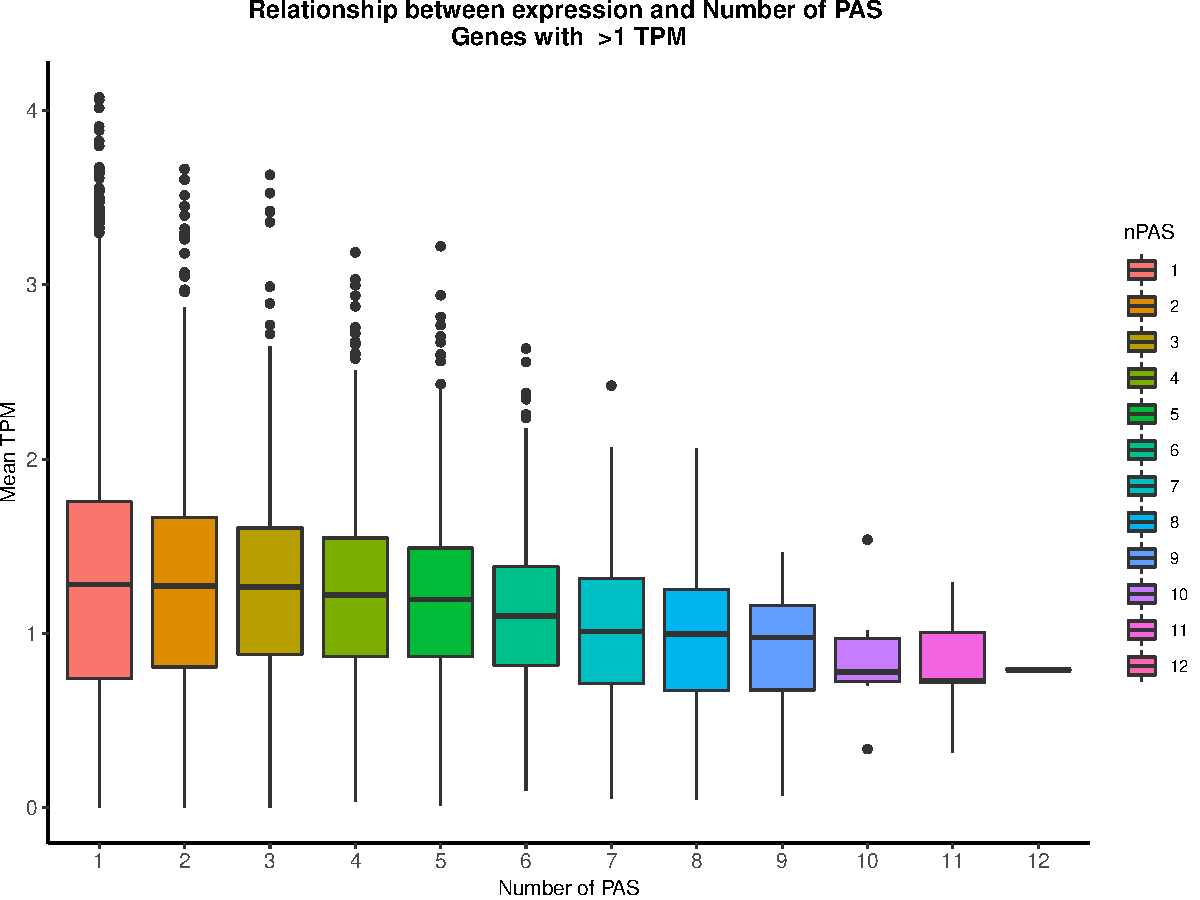
\includegraphics[width=5in]{img/ch02/Fig1_figuresupplement1.pdf}
\caption[Relationship between Number of PAS and gene expression]{\textbf{Relationship between Number of PAS and gene expression} Relationship between number of PAS identified in our study and gene expression levels (TPM) as measured from GEUVADIS YRI LCLs \citep{lappalainen_transcriptome_2013}. Genes with mean TPM $<$ 1 across individuals were considered not expressed and thus were removed for this analysis.}
\label{fig:ch02-pas-exp}
\end{figure}
\clearpage

\begin{figure}[!htb]
\centering 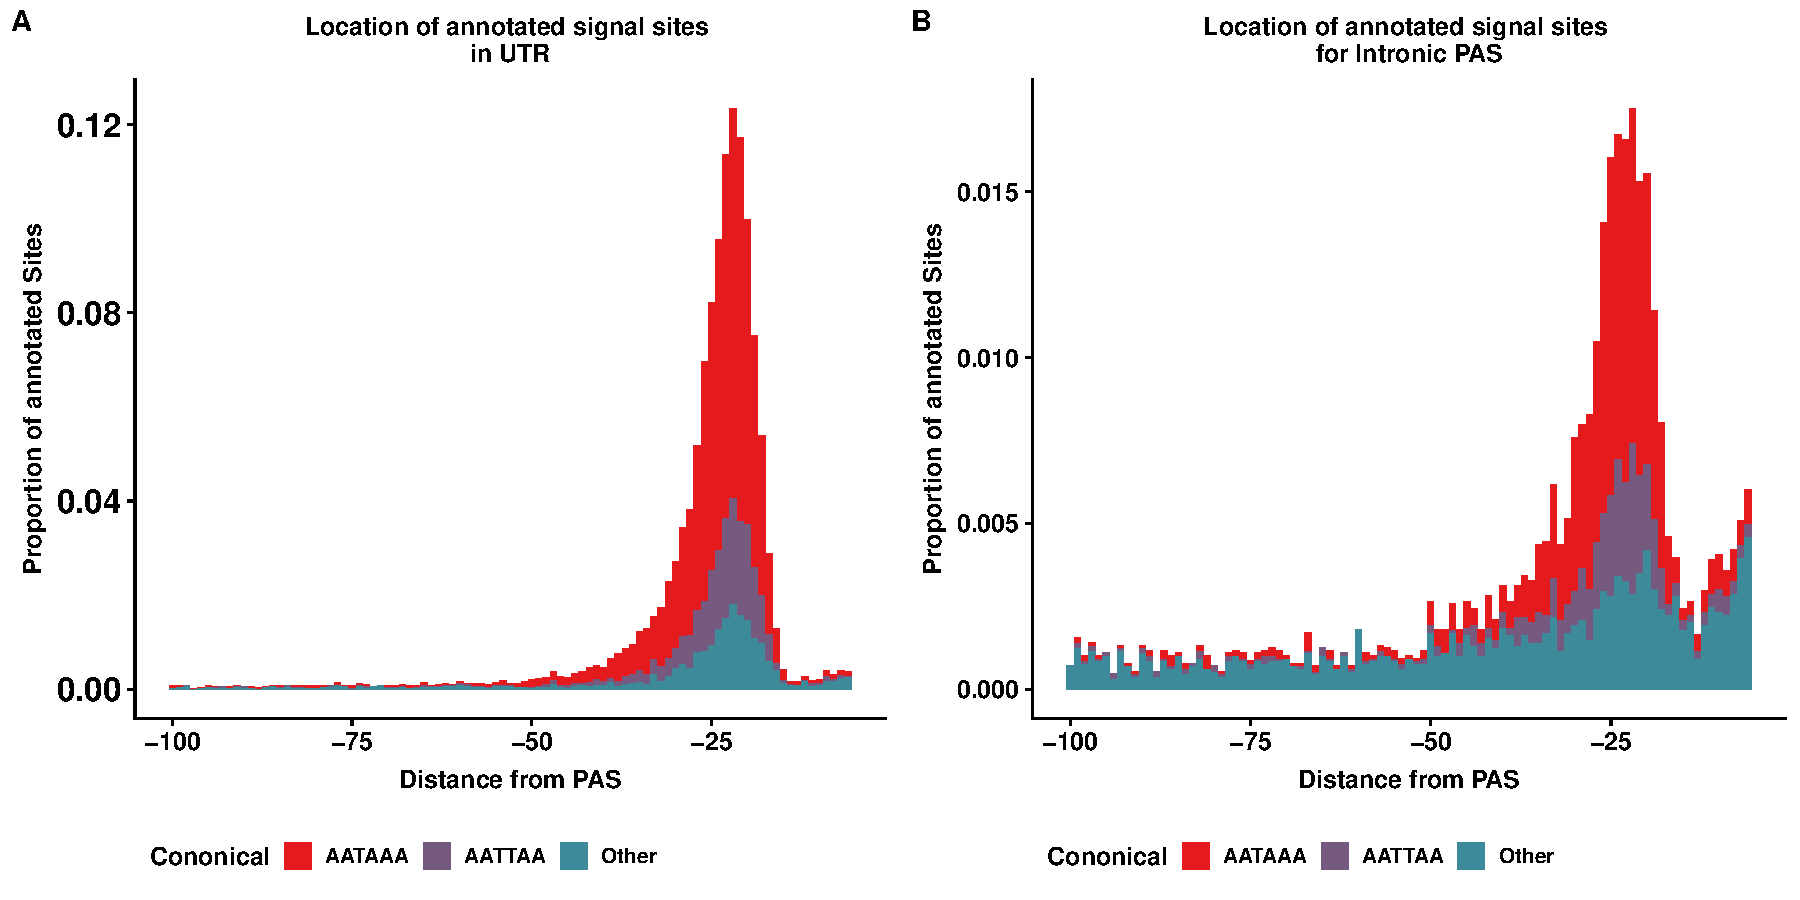
\includegraphics[width=5in]{img/ch02/Fig1_figuresupplement2.pdf}
\caption[Distribution of signal sites upstream of PAS. Supplement to Figure 2.1D]{\textbf{Distribution of signal sites upstream of PAS. Supplement to Figure 2.1D} {\bf (A)} Stacked density plot showing the signal site distribution for PAS in 3' UTR. Other signal sites are AAAAAA, AAAAAG, AATACA, AATAGA, AATATA, ACTAAA, AGTAAA, CATAAA, GATAAA, TATAAA. {\bf (B)} Stacked density plot showing the signal site distribution for PAS in introns. Other signal sites are AAAAAA, AAAAAG, AATACA, AATAGA, AATATA, ACTAAA, AGTAAA, CATAAA, GATAAA, TATAAA.}
\label{fig:SS}
\end{figure}
\clearpage

\begin{figure}[!htb]
\centering
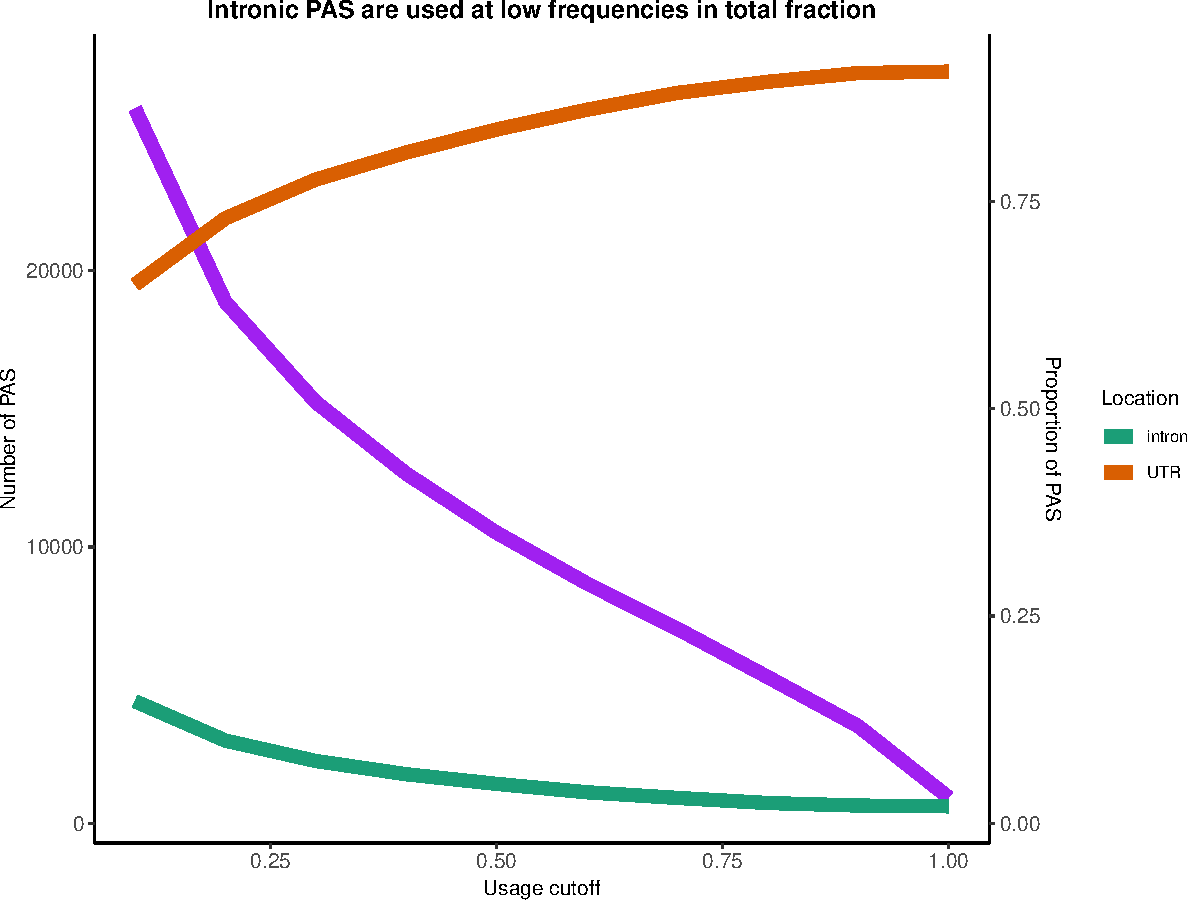
\includegraphics[width=5in]{img/ch02/Fig1_figuresupplement3.pdf}
\caption[Proportion of PAS in 3' UTRs and introns as predicted from total 3' Seq. Additional figures corresponding to Figure 2.1E.]{\textbf{Proportion of PAS in 3' UTRs and introns as predicted from total 3' Seq. Additional figures corresponding to Figure 2.1E.} Number of PAS identified with usage larger than the usage cutoff (x axis) in the total mRNA fraction (purple). Proportion of PAS in introns when PAS are filtered by total usage (green). Proportion of PAS in 3' UTRs when PAS are filtered by total usage (orange).}
\label{fig:totaUsage}
\end{figure}
\clearpage

\begin{figure}[!htb]
\centering 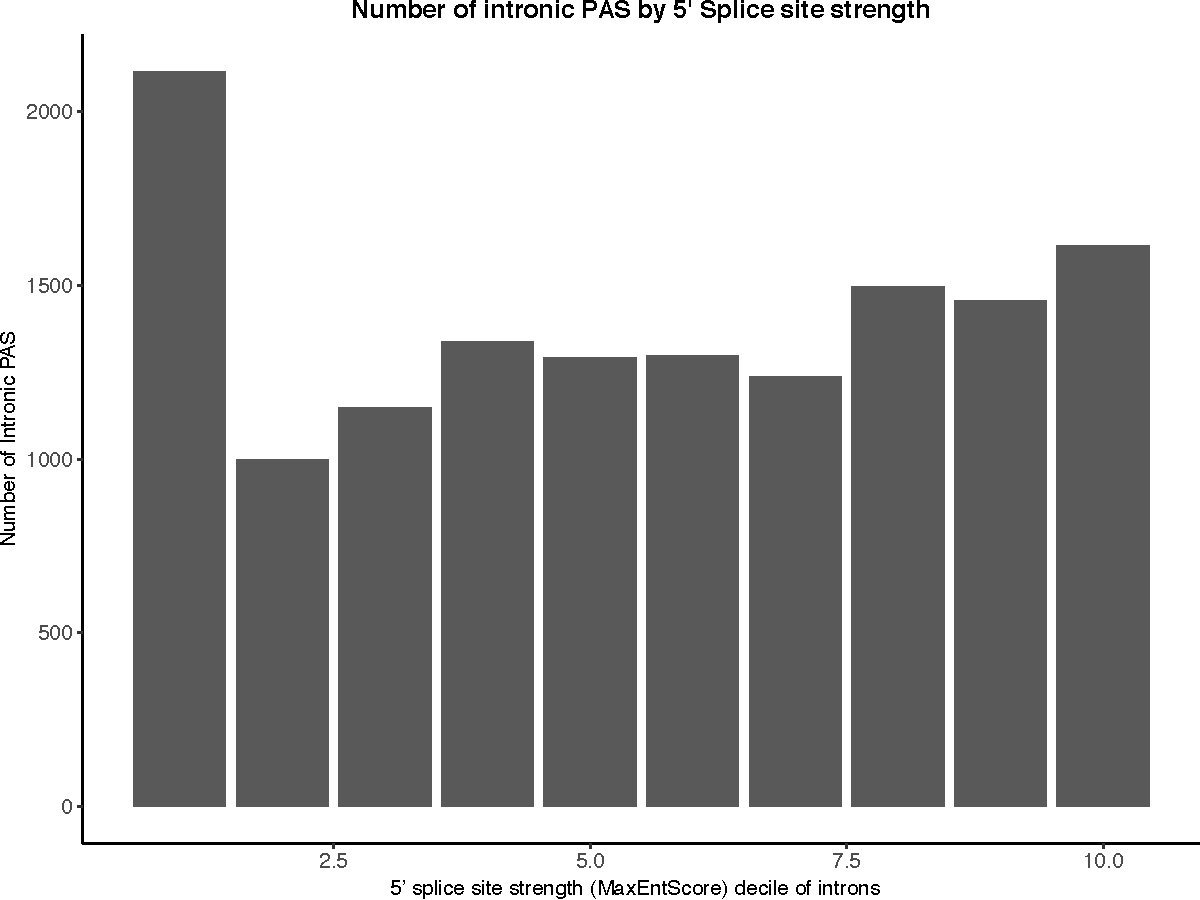
\includegraphics[width=5in]{img/ch02/Fig1_figuresupplement4.pdf}
\caption[Intronic PAS 5' Splice site strength]{\textbf{Intronic PAS 5' Splice site strength} Intronic PAS are enriched in introns with the weakest 5' splice sites. Splice site strengths for all introns were calculated using MaxEntScore \citep{yeo_maximum_2004}}.
\label{fig:splicesite}
\end{figure}
\clearpage

\begin{figure}[!htb]
\centering 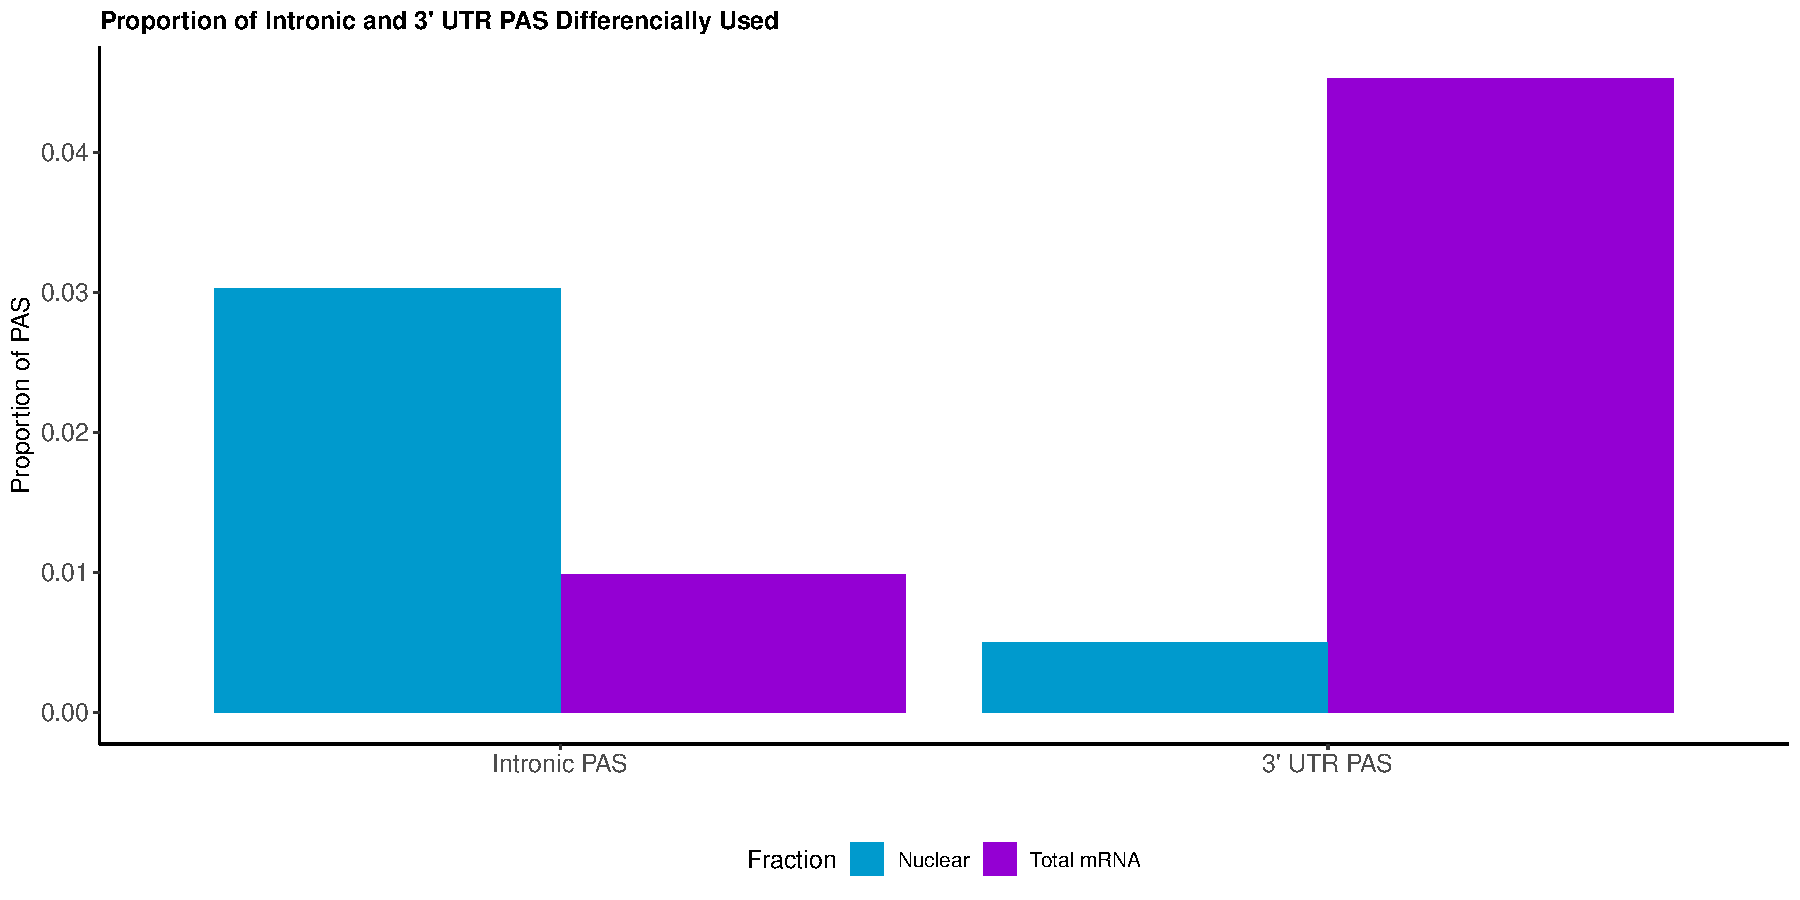
\includegraphics[width=5in]{img/ch02/Fig1_figuresupplement5.pdf}
\caption[Location of PAS differentially used]{\textbf{Location of PAS differentially used} We adapted LeafCutter to identify genes with significant differential usage of PAS between the total and nuclear fraction. The majority of PAS preferentially used in the nuclear fraction are intronic, whereas the majority of PAS preferentially used in the total fraction lie in the 3' UTR. }
\label{fig:locdPAS}
\end{figure}
\clearpage


\begin{figure}[!htb]
\centering 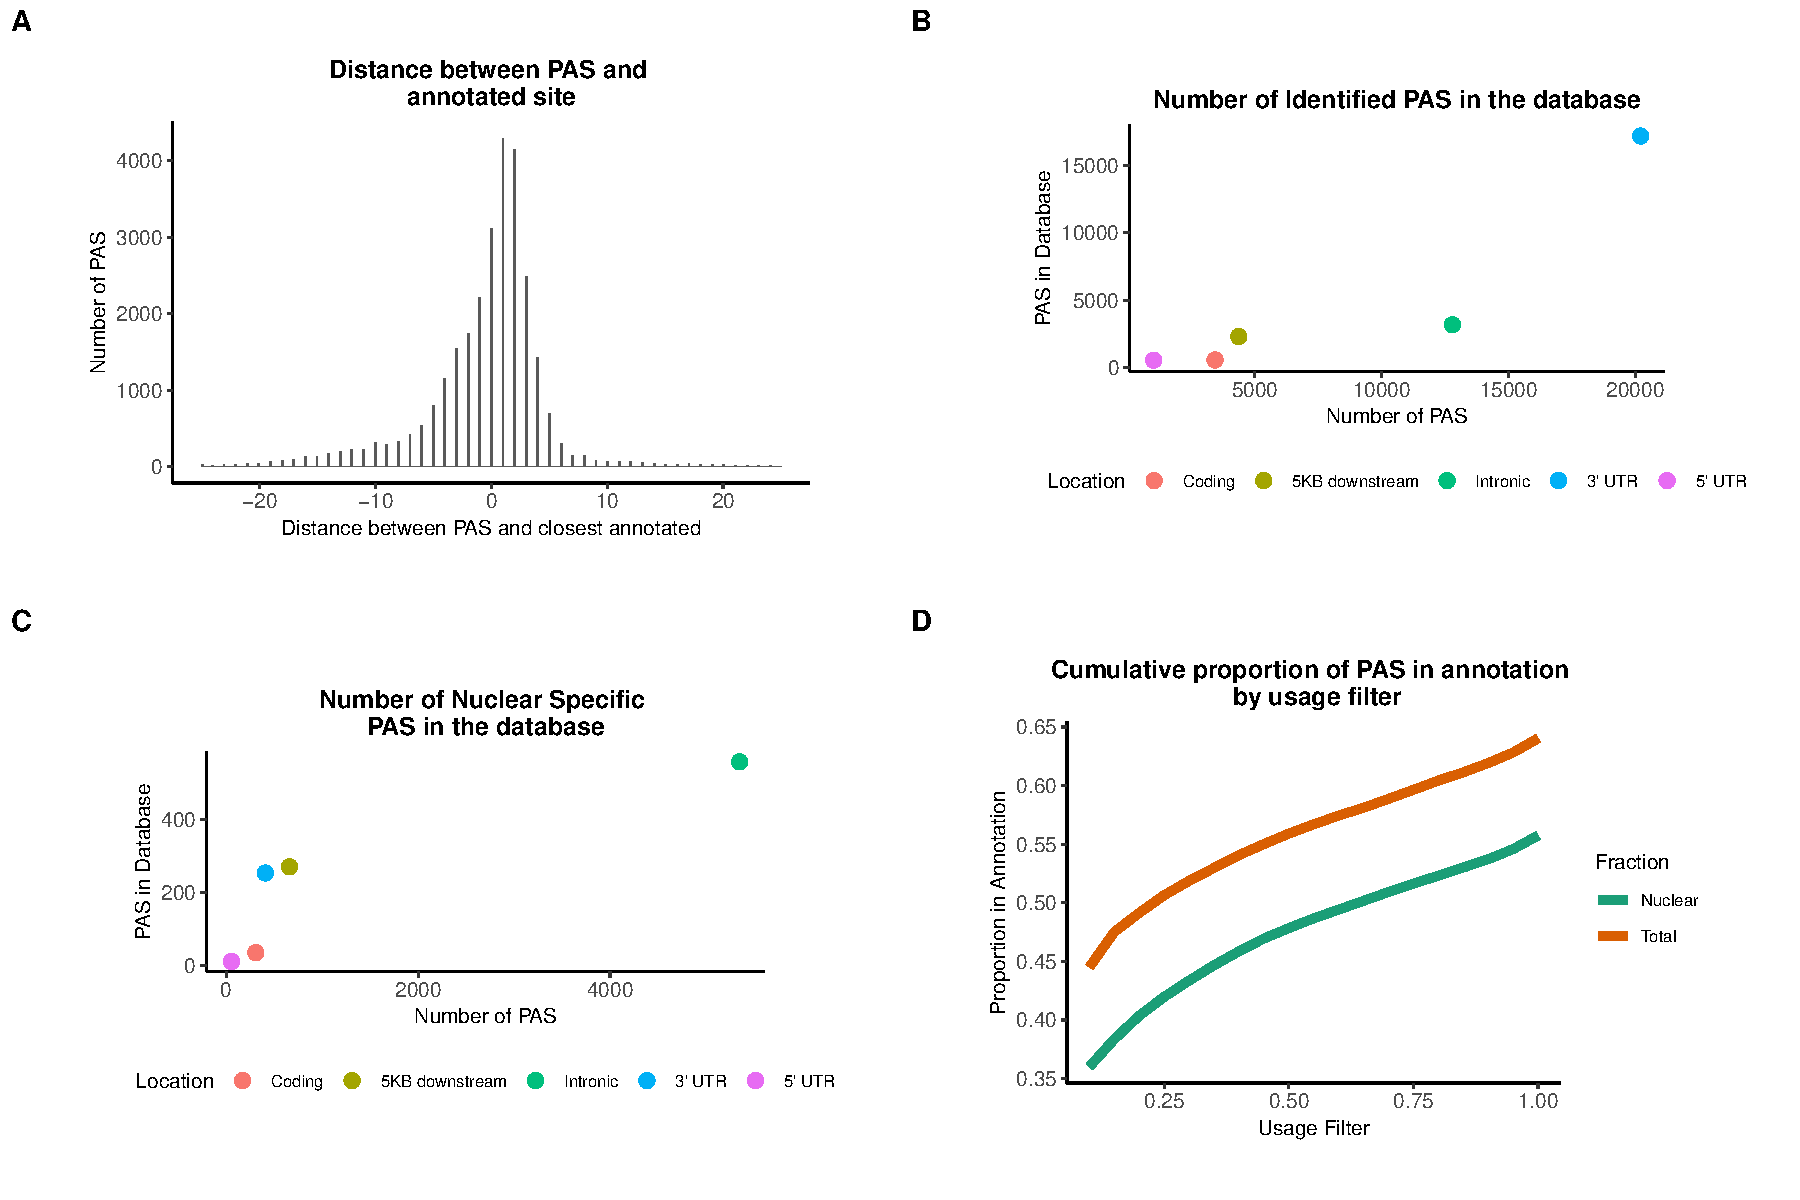
\includegraphics[width=5in]{img/ch02/Fig1_figuresupplement6.pdf}
\caption[Comparison of our 3'-Seq PAS to previous PAS annotations]{\textbf{Comparison of our 3' Seq PAS to previous PAS annotations} {\bf (A)} Distribution of distance between PAS and closest annotated site in the annotation database (PolyA\_DB release 3.2) \citep{wang_polya_db_2018}. {\bf (B)} Scatter plot showing the number of PAS we identified in our study (X axis) versus the number of PAS in the PolyA database (Y axis) separated by genomic location (colors). {\bf (C)} Scatter plot showing the number of nuclear-specific PAS we identified in our study versus the number of PAS in the PolyA database separated by genomic location (colors). The vast majority of nuclear-specific PAS are intronic. {\bf (D)} Proportion of PAS present in the PolyA database by usage in nuclear (green) or total (orange) mRNA fraction.}
\label{fig:compAnno}
\end{figure}
\clearpage


\begin{figure}[!htb]
\centering 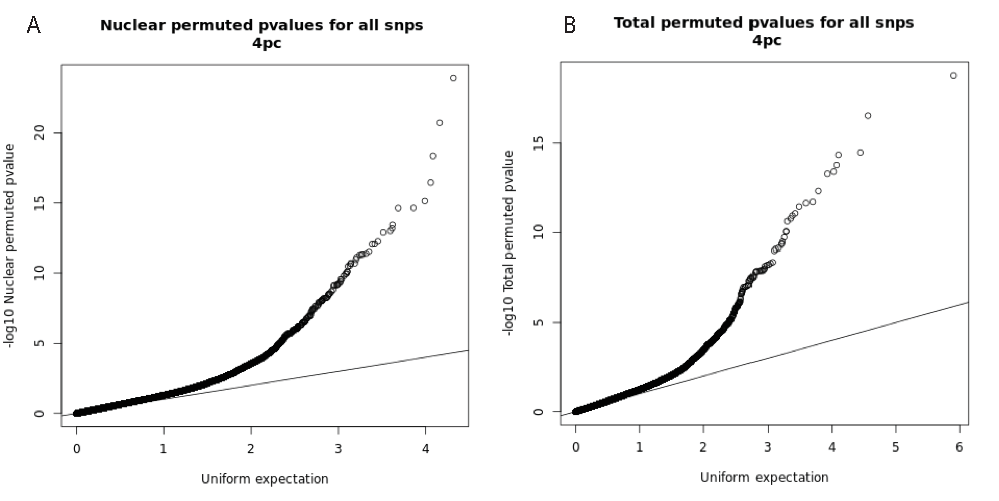
\includegraphics[width=5in]{img/ch02/Fig2_figuresupplement1.pdf}
\caption[Q-Q plots for apaQTLs]{\textbf{Q-Q plots for apaQTLs} {\bf (A)} Q-Q plot for nuclear apaQTLs, plotting adjusted p-values of the top SNP PAS associations. {\bf (B)} Q-Q plot for total apaQTLs, plotting adjusted p-values of the top SNP PAS associations.}
\label{fig:QQplots}
\end{figure}
\clearpage

\begin{figure}[!htb]
\centering
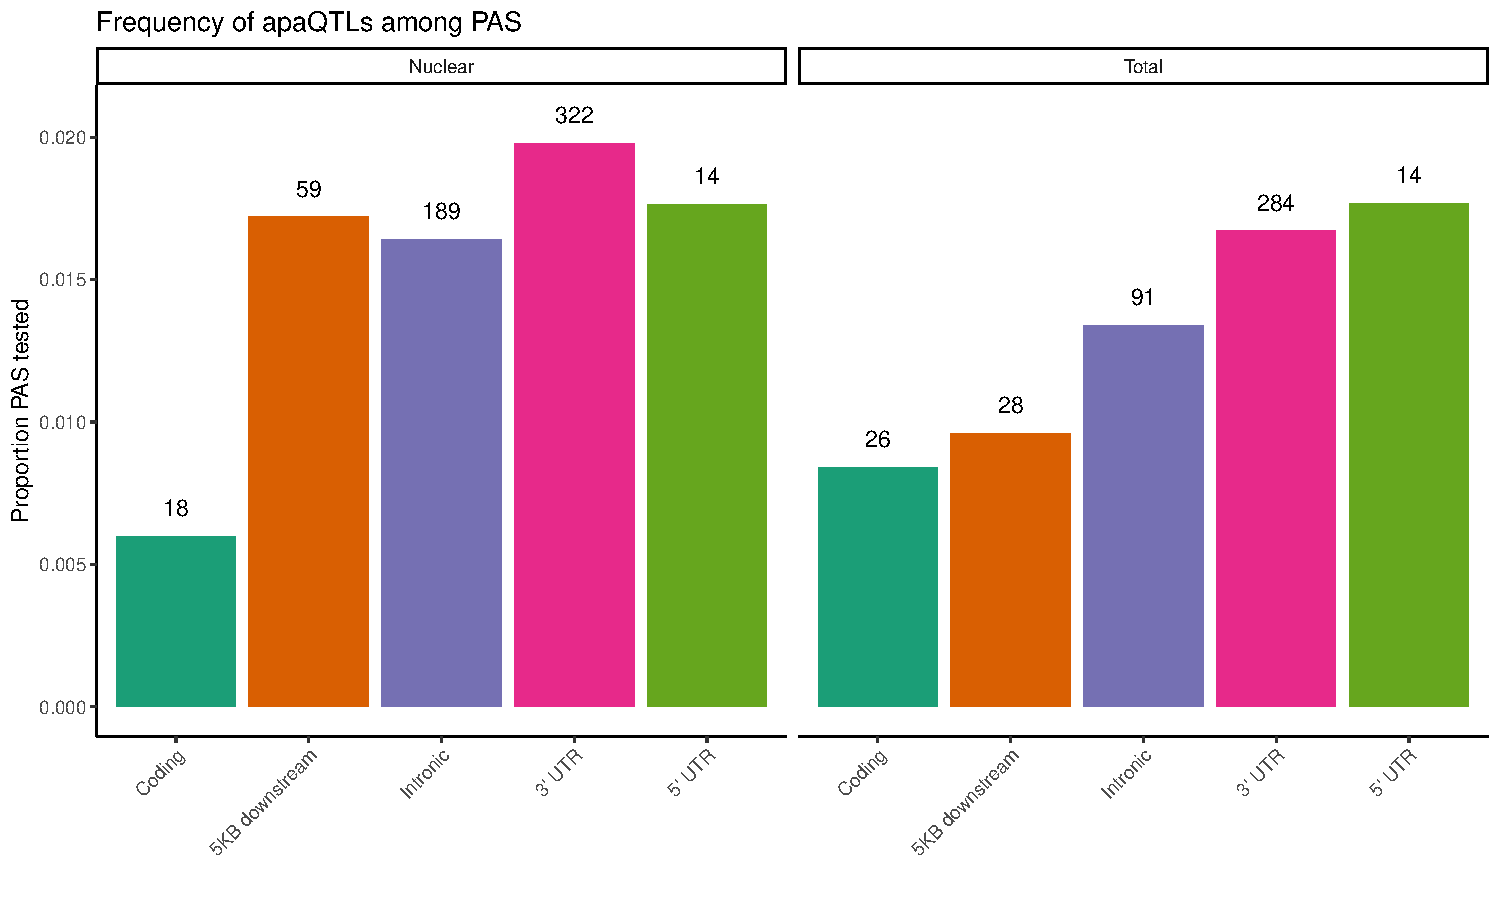
\includegraphics[width=5in]{img/ch02/Fig2_figuresuplement2.pdf}
\caption[Proportion of PAS tested with an apaQTL]{\textbf{Proportion of PAS tested with an apaQTL} Proportion of PAS in different genomic locations with a significant apaQTL. The numbers above each bar represent the number of identified apaQTL for each location. }
\label{fig:propPASdAPA}
\end{figure}
\clearpage

\begin{figure}[!htb]
\centering
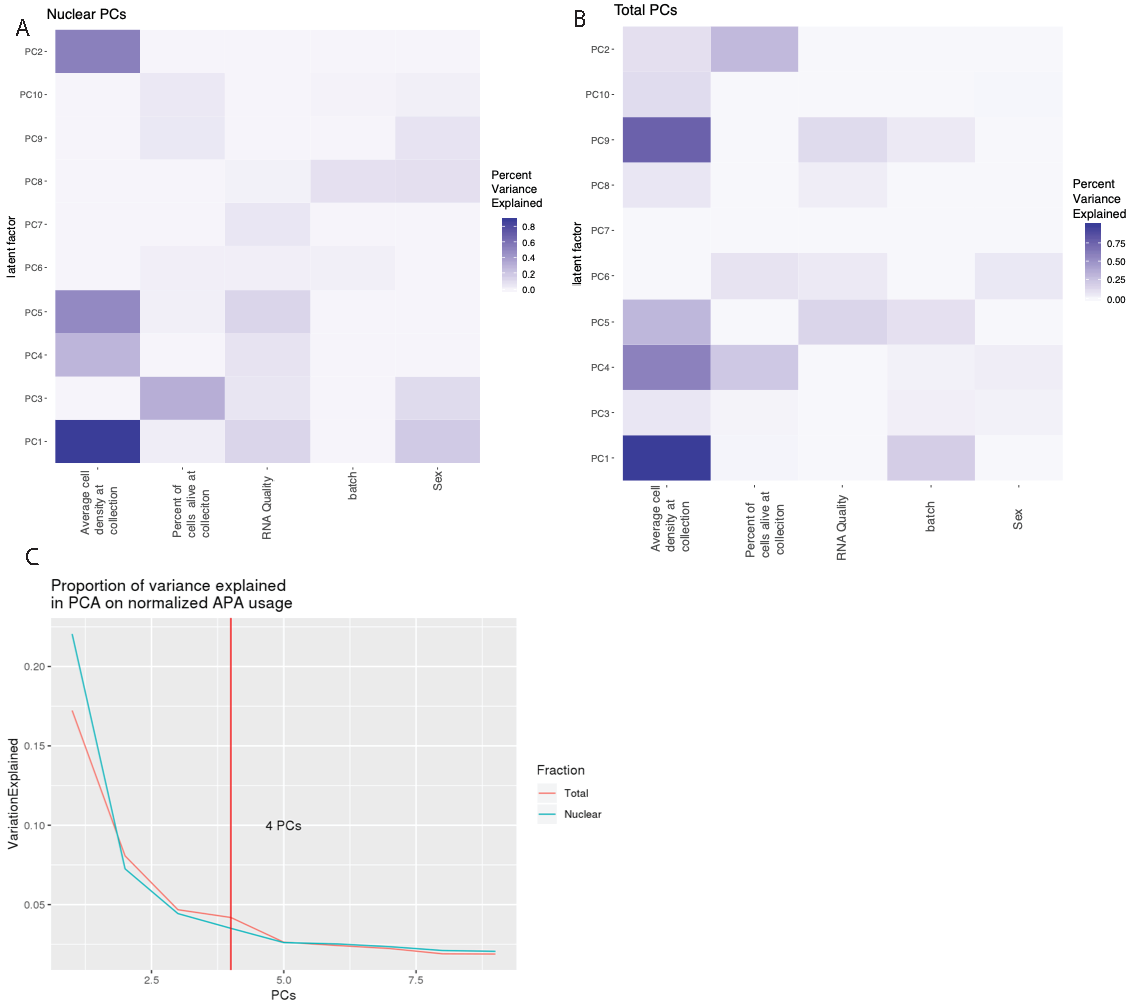
\includegraphics[width=5in]{img/ch02/Fig2_figuresupplement3.pdf}
\caption[Analysis of the PCs of APA usage]{\textbf{Analysis of the PCs of APA usage} {\bf (A)} Proportion of variance explained in the 10 first PCs by experimental variables in nuclear APA usage. We used a linear model to look at correlation between PC and each covariate. {\bf (B)} Proportion of variance explained in the 10 first PCs by experimental variables in total APA usage. We used a linear model to look at correlation between PC and each covariate. {\bf (C)} Proportion of variance explained by each PC in APA usage. Vertical line represents the number of PCs used as covariates in our apaQTL analysis.}
\label{fig:PCA}
\end{figure}
\clearpage

\begin{figure}[!htb]
\centering
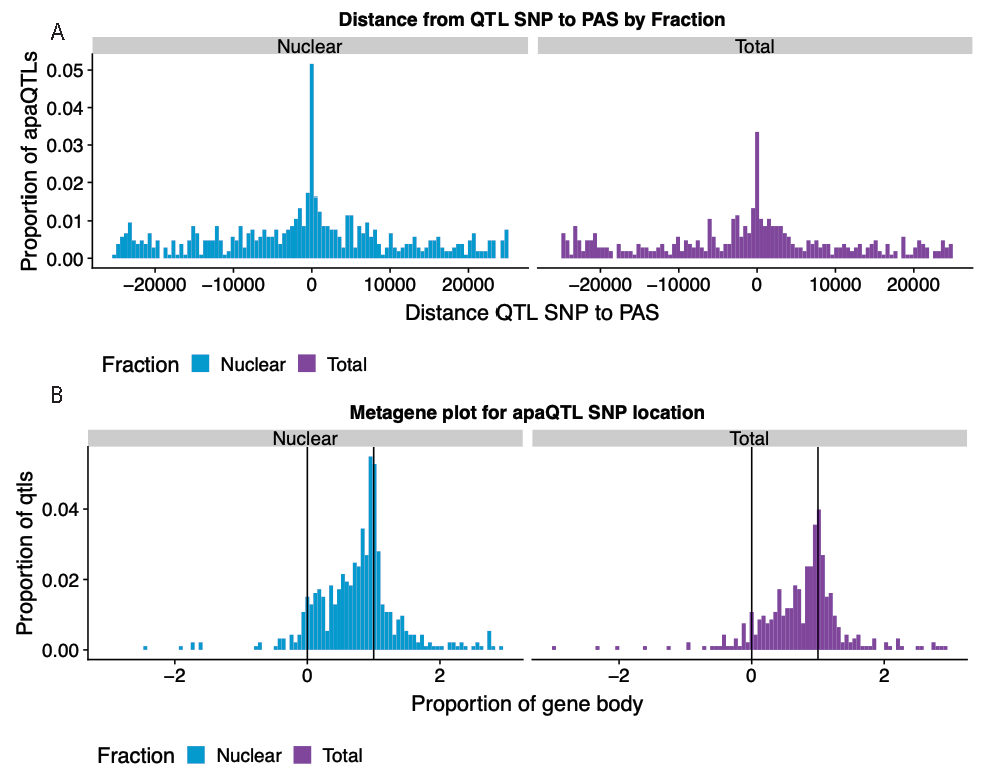
\includegraphics[width=5in]{img/ch02/Fig2_figuresupplement4.pdf}
\caption[apaQTLs in both fractions are associated with PAS near SNP and at the transcription end site.  Supplement to Figure 2.2B and 2.2C.]{\textbf{apaQTLs in both fractions are associated with PAS near SNP and at the transcription end site.  Supplement to Figure 2.2B and 2.2C.} {\bf (A)} Histogram showing the distribution of the distance between lead apaQTL SNP and the PAS, separated by mRNA fraction. {\bf (B)} Histogram showing the distribution of the distance between lead apaQTL SNP and gene features, where 0 represents annotated TSS and 1 represents annotated TES, separated by mRNA fraction.}
\label{fig:totQTLloc}
\end{figure}
\clearpage

\begin{figure}[!htb]
\centering
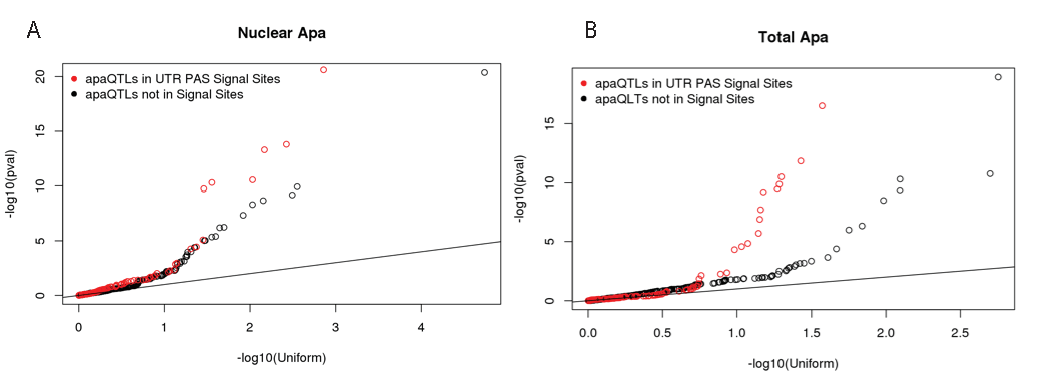
\includegraphics[width=5in]{img/ch02/Fig2_figuresupplement5.pdf}
\caption[Signal site disruption]{\textbf{Signal site disruption} {\bf (A)} Q-Q plot showing the nuclear apaQTL p-values for SNP in signal sites upstream of 3' UTR PAS compared to matched SNPs (equal distance) upstream of a set of 3' UTR PAS without identified signal sites. {\bf (B)} Similar to panel A, but for total apaQTLs.}
\label{fig:ssDisrupt}
\end{figure}
\clearpage

\begin{figure}[!htb]
\centering
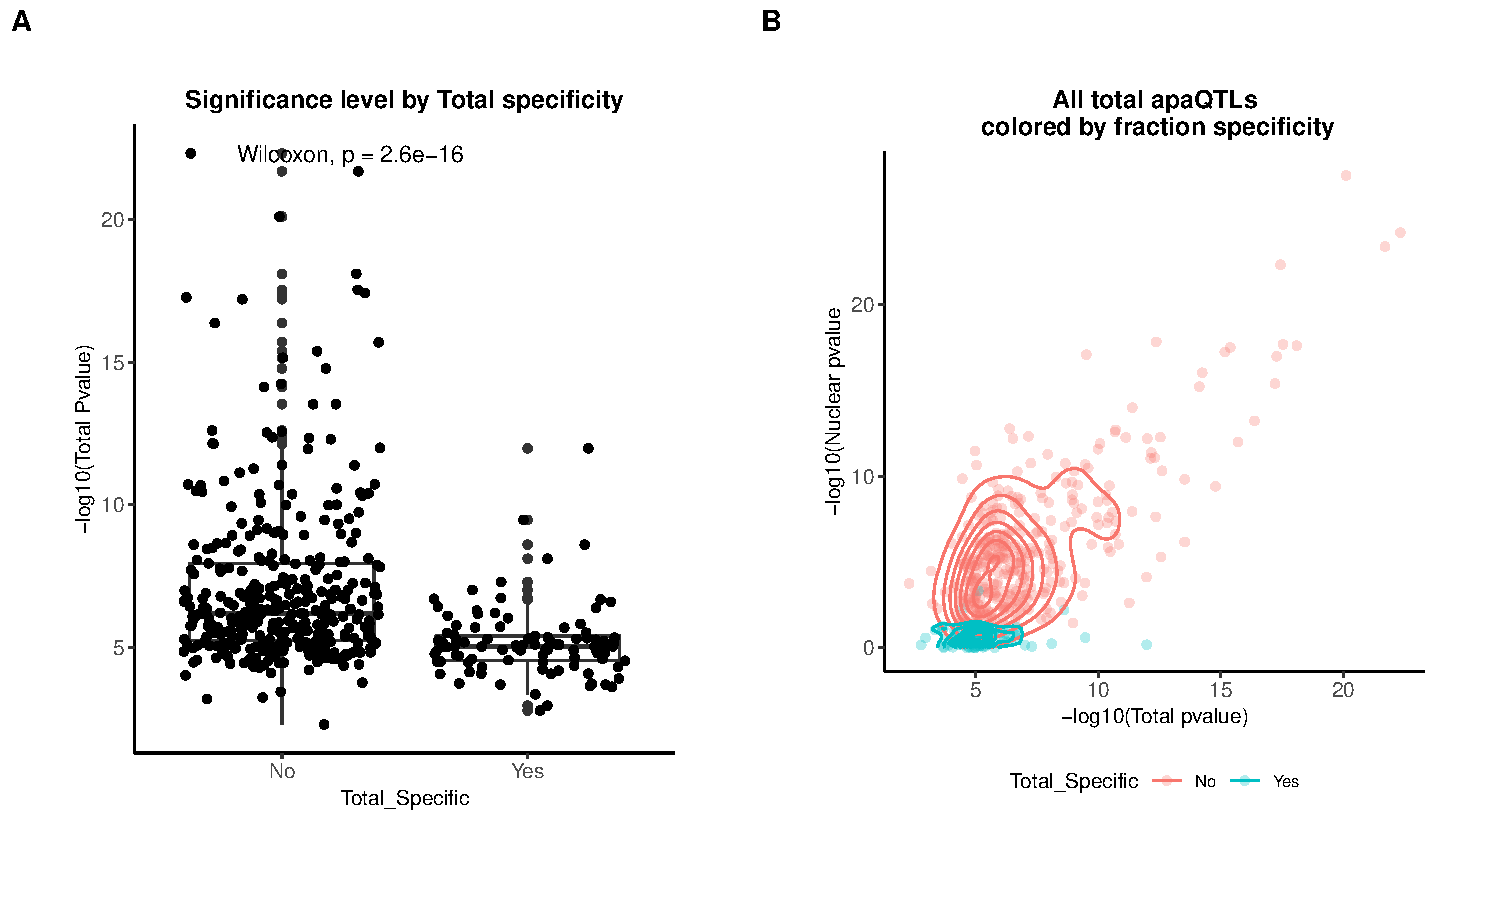
\includegraphics[width=5in]{img/ch02/Fig2_figuresupplement6.pdf}
\caption[Total mRNA specific apaQTLs show weaker association than do shared apaQTLs]{\textbf{Total mRNA specific apaQTLs show weaker association than do shared apaQTLs} {\bf (A)} Boxplot showing the -log10(p-value) of the nominal total apaQTL associations separated by whether the association is also identified in the nuclear mRNA fraction. ApaQTLs that are total-specific have significantly weaker associations. {\bf (B)} Scatter plot showing the relationship between the -log10(p-valued) of the apaQTL associations in both mRNA fractions for total mRNA apaQTLs. Dots and densities are colored by whether the apaQTL is total-specific or shared. Total-specific apaQTLs are likely not detected in the nuclear fraction due to a lack of power.}
\label{fig:totSpeWeak}
\end{figure}
\clearpage

\begin{figure}[!htb]
\centering
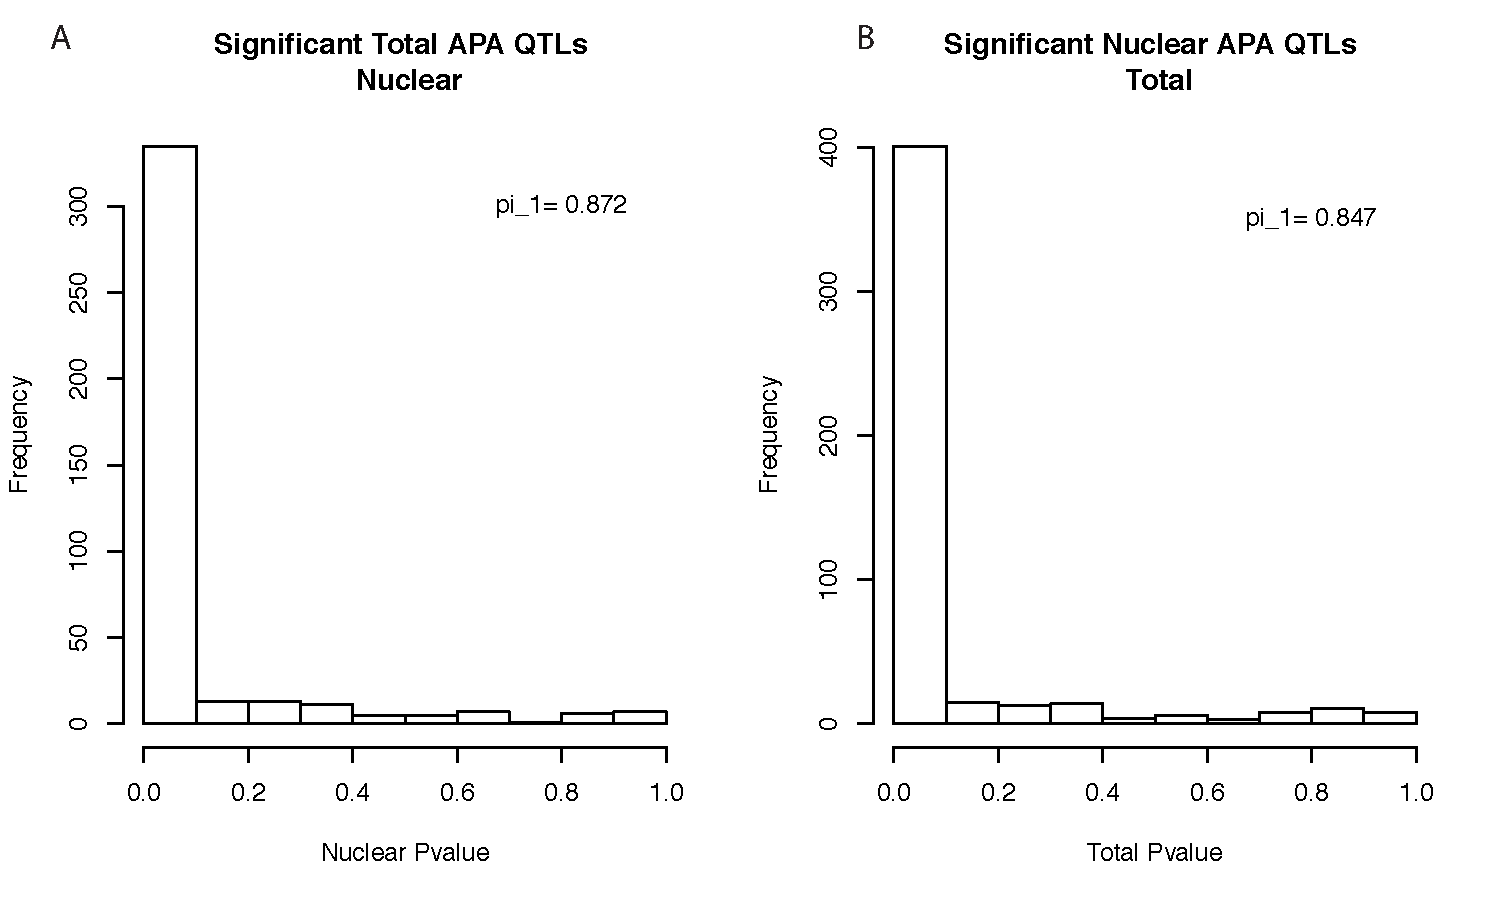
\includegraphics[width=5in]{img/ch02/Fig2_figuresupplement7.pdf}
\caption[apaQTL sharing between fractions]{\textbf{apaQTL sharing between fractions} {\bf (A)}	 Histogram showing the P-value distribution of the apaQTL associations between the lead total apaQTL SNP and the corresponding PAS ascertained using our 3'-Seq data from the nuclear mRNA fraction. Values were calculated based on PAS tested in both fractions (403 of 443). Results are robust to using all PAS $(pi_1=0.842)$ {\bf (B)} Histogram showing the P-value distribution of the apaQTL associations between the lead nuclear apaQTL SNP and the corresponding PAS ascertained using our 3'-Seq data from the total mRNA fraction. Values calculated based on PAS tested in both fractions. (483 of 602) Results are robust to using all PAS $(pi_1=0.825)$}
\label{fig:QTLshare}
\end{figure}
\clearpage


\begin{figure}[!htb]
\centering
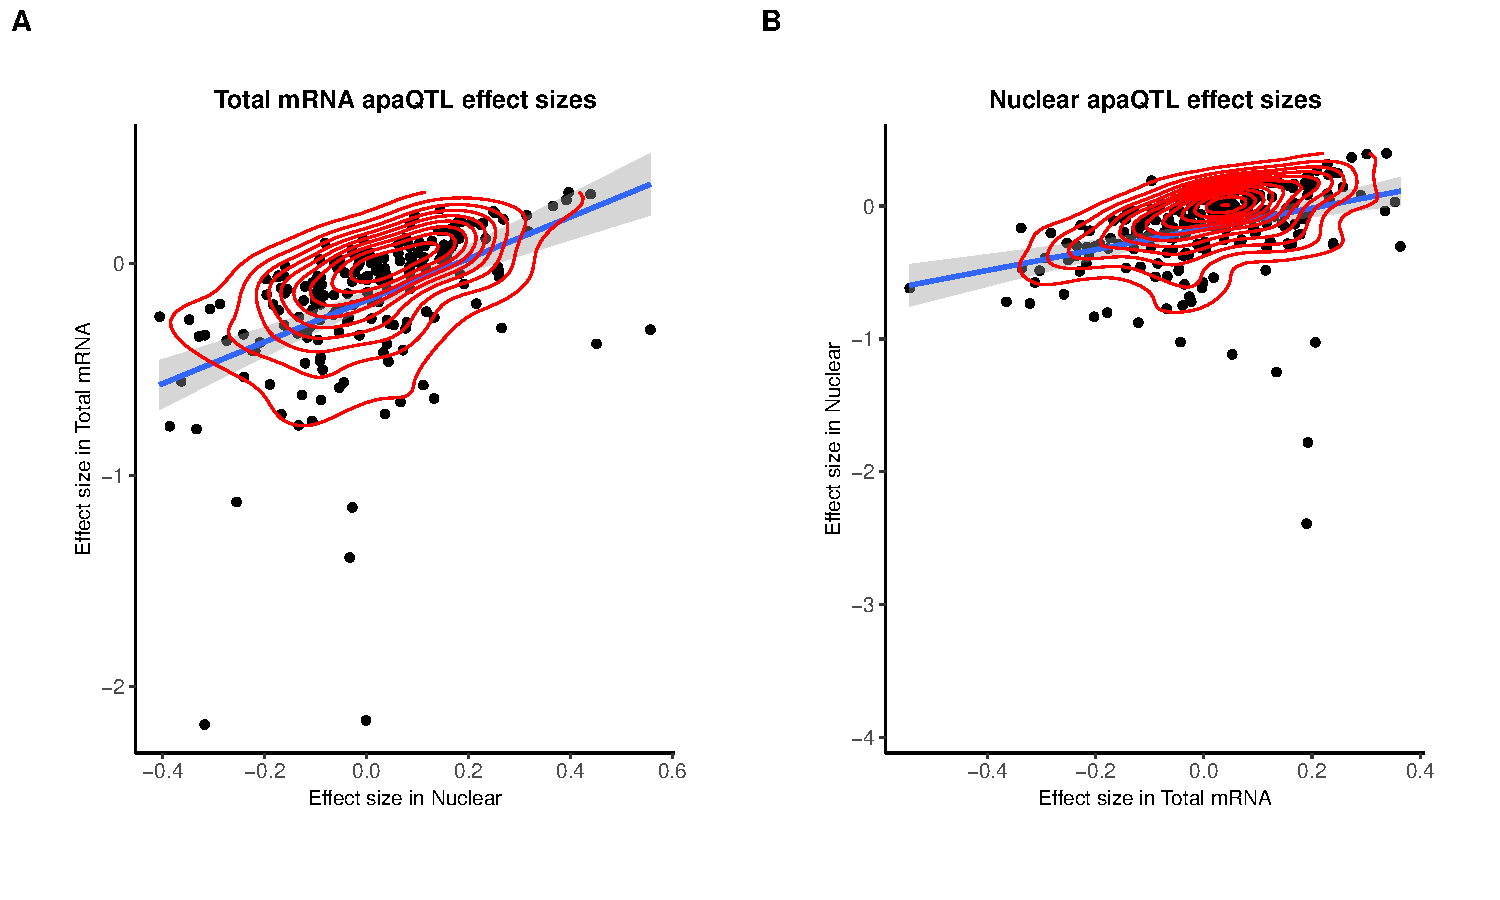
\includegraphics[width=5in]{img/ch02/Fig2_figuresupplement8.pdf}
\caption[Correlation of effect sizes for apaQTLs discovered in total and nuclear mRNA fractions]{\textbf{Correlation of effect sizes for apaQTLs discovered in total and nuclear mRNA fractions} {\bf (A)} Normalized effect sizes ascertained in total mRNA and nuclear fraction of total apaQTLs tested in both fractions. {\bf (B)} Normalized effect sizes ascertained in total mRNA and nuclear fraction for nuclear apaQTLs tested in both fractions.}
\label{fig:apaQTLcorr}
\end{figure}
\clearpage

\begin{figure}[!htb]
\centering
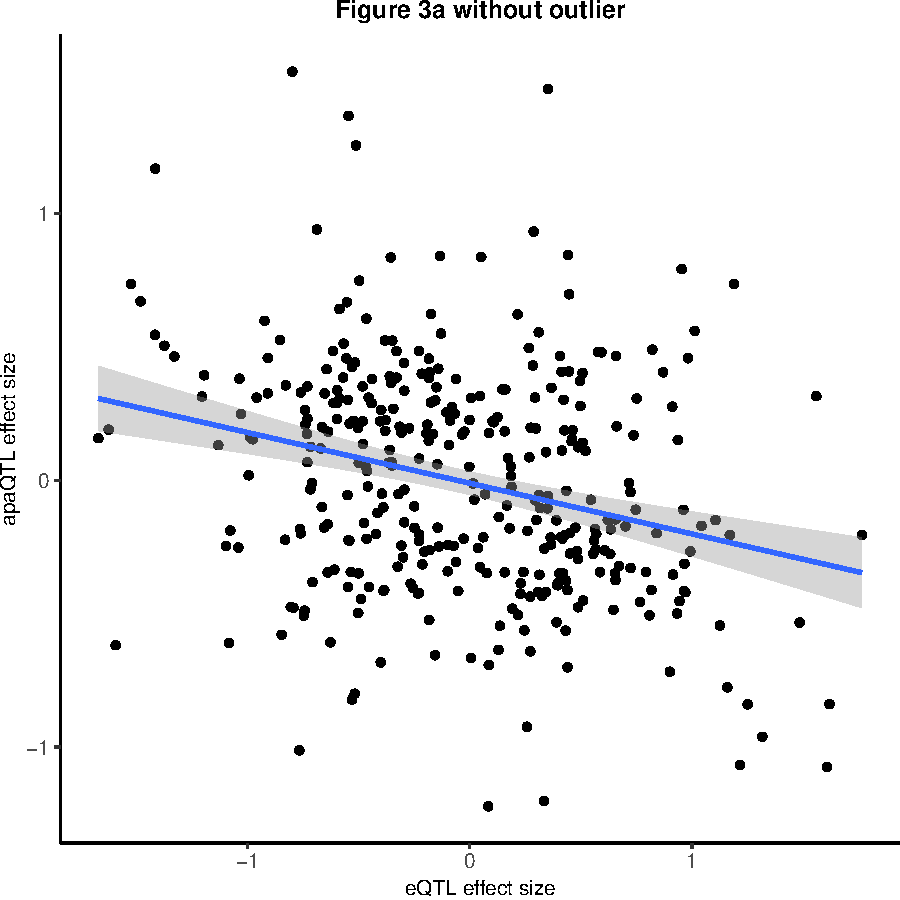
\includegraphics[width=5in]{img/ch02/Fig3_figuresupplement1.pdf}
\caption[Figure 2.3A without outlier SNP]{\textbf{Figure 2.3A without outlier SNP} Scatter plot showing the relationship between intronic nuclear apaQTL effect size and eQTL effect size after removing outlier SNPs (Filtered for SNPs with eQTL effect size $<$ -2.0).}
\label{fig:3anooutlier}
\end{figure}
\clearpage

\begin{figure}[!htb]
\centering
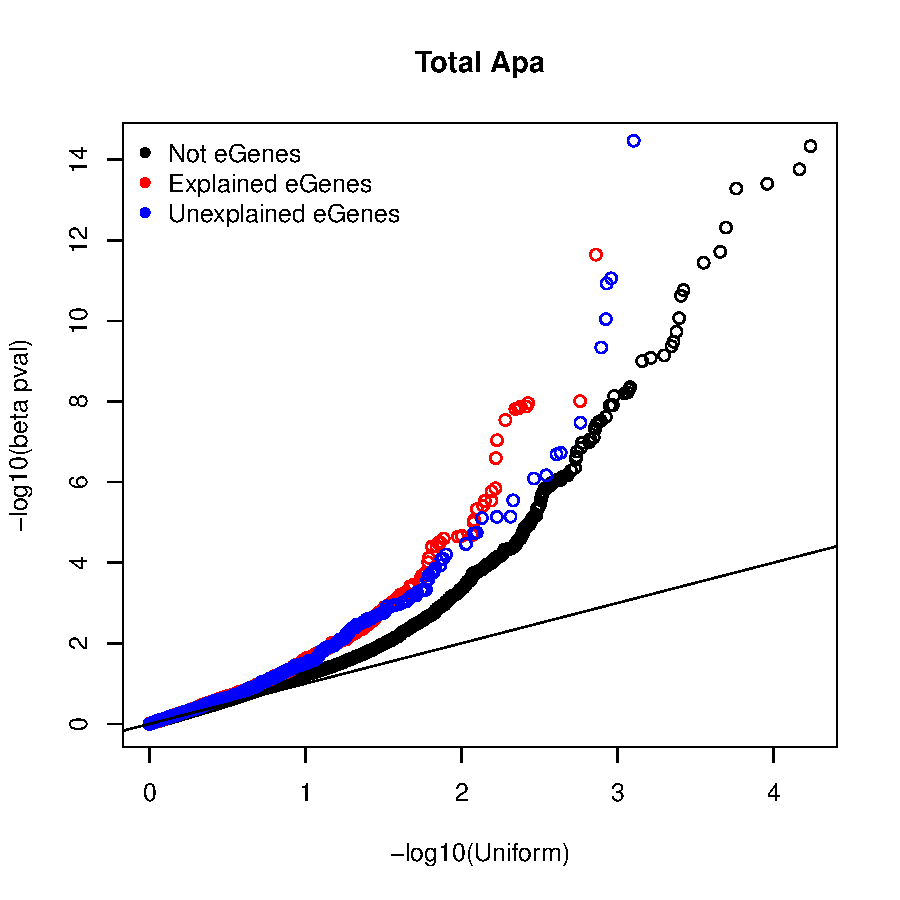
\includegraphics[width=5in]{img/ch02/Fig3_figuresupplement2.pdf}
\caption[Overlap between apaQTLs in total fraction and eQTLs, supplement to Figure 2.3B]{\textbf{Overlap between apaQTLs in total fraction and eQTLs, supplement to Figure 2.3B} QQ-plot showing the total apaQTL (adjusted) p-values separated by whether the gene harbors an explained (red) or unexplained (blue) eQTLs. We observe an enrichment for low apaQTL association p-values in genes with eQTLs compared to all tested genes (black). }
\label{fig:totunexp}
\end{figure}
\clearpage

\begin{figure}[!htb]
\centering
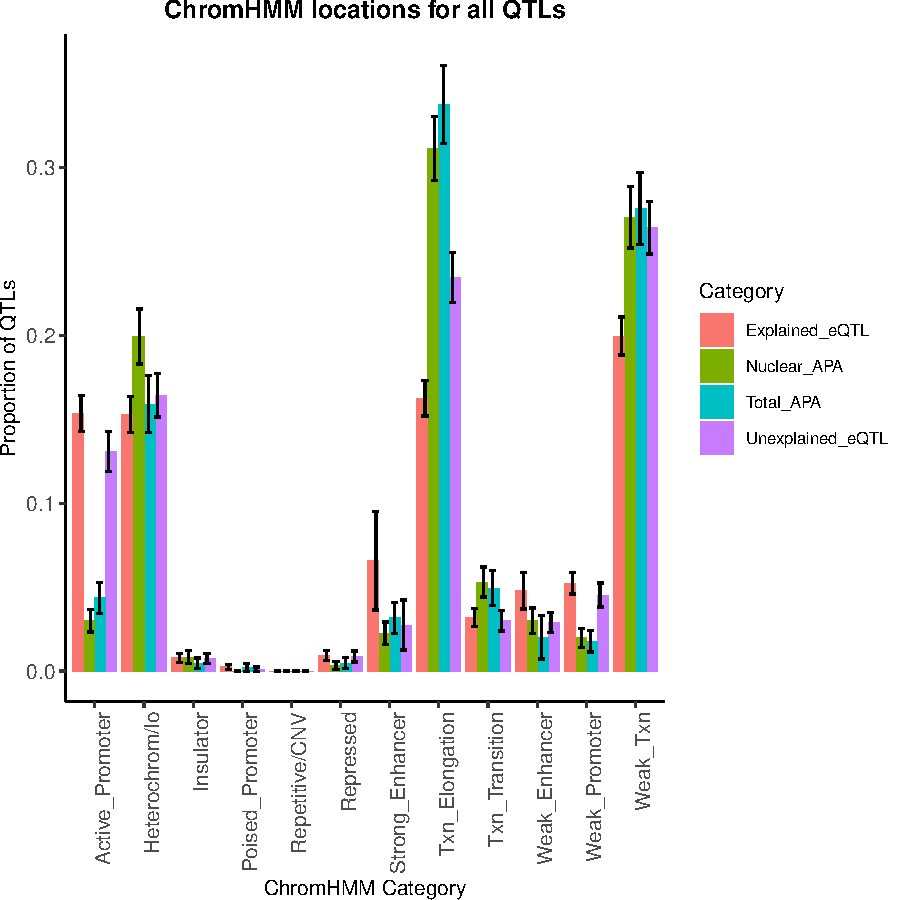
\includegraphics[width=5in]{img/ch02/Fig3_figuresupplement3.pdf}
\caption[Proportion of apaQTLs and eQTLs by Chromatin state]{\textbf{Proportion of apaQTLs and eQTLs by Chromatin state} Bar plot showing the proportion of apaQTLs located in each of the 12 chromatin states from chromHMM. We find that the location profile of apaQTLs is more similar to that of unexplained eQTLs than that of explained eQTLs. Error bars represent the 95\% confidence interval for each point estimate from bootstrapping 1,000 times.}
\label{fig:chromHMM}
\end{figure}
\clearpage

\begin{figure}[!htb]
\centering
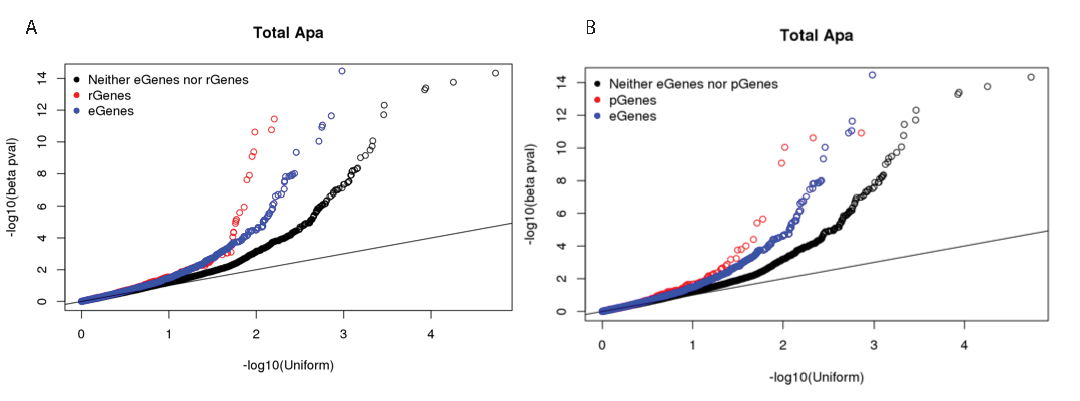
\includegraphics[width=5in]{img/ch02/Fig4_figuresupplement1.pdf}
\caption[Overlap between apaQTLs in total fraction and eQTLs, rQTLs and pQTLs supplement to Figure 2.4A]{\textbf{Overlap between apaQTLs in total fraction and eQTLs, rQTLs and pQTLs supplement to Figure 2.4A} {\bf (A)} QQ-plot showing the total apaQTL (adjusted) p-values separated by whether the corresponding gene has a ribosome occupancy QTL (red) or an eQTL (red). We see an enrichment for low apaQTL p-values in genes with either association. {\bf (B)} QQ-plot showing the total apaQTL (adjusted) p-values separated by whether the corresponding gene has a protein expression QTL (red) or an eQTL (red). We see an enrichment for low apaQTL p-values in genes with either association.}
\label{fig:totpgene}
\end{figure}
\clearpage

\begin{figure}[!htb]
\centering
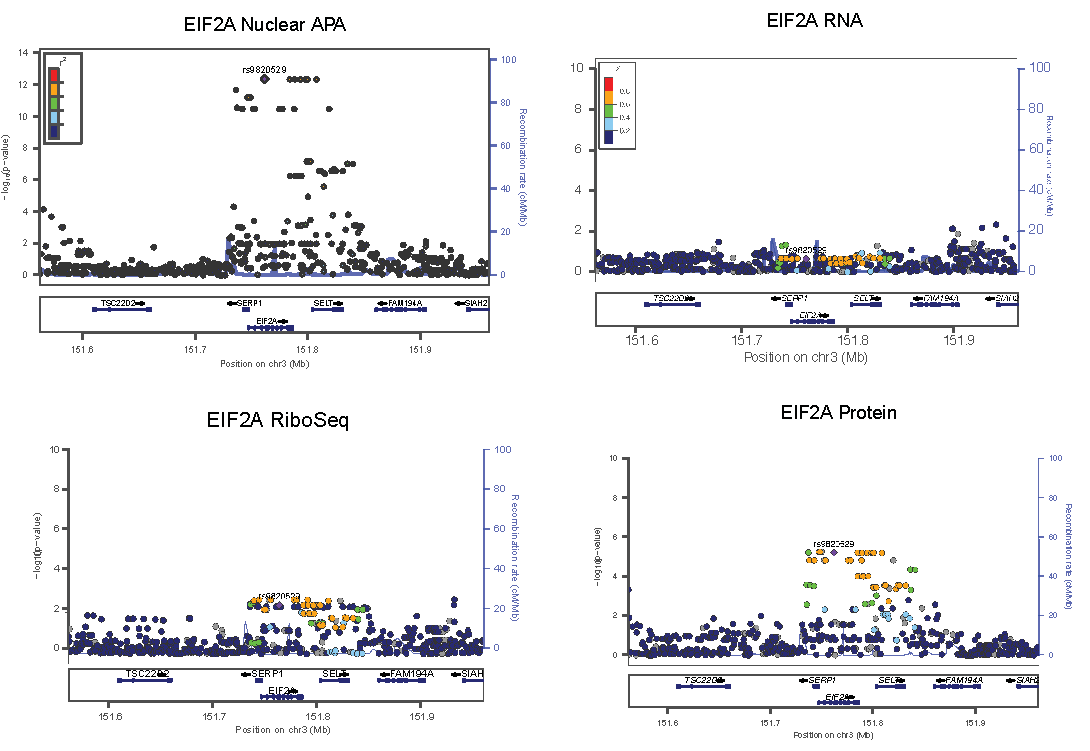
\includegraphics[width=5in]{img/ch02/Fig4_figuresupplement2.pdf}
\caption[LocusZoom plots for EIF2A molecular associations, Supplement to Figure 2.4B]{\textbf{LocusZoom plots for EIF2A molecular associations, Supplement to Figure 2.4B} LocusZoom plots for EIF2A apaQTL in Figure 2.4B along with associations with RNA expression, ribosome occupancy (ribo-seq), and protein expression as determined using normalized data from Li et al. 2016 \citep{li_rna_2016}. LD patterns were colored according to the HapMap YRI lines.}
\label{fig:locuszoom}
\end{figure}
\clearpage



\begin{figure}[!htb]
\centering
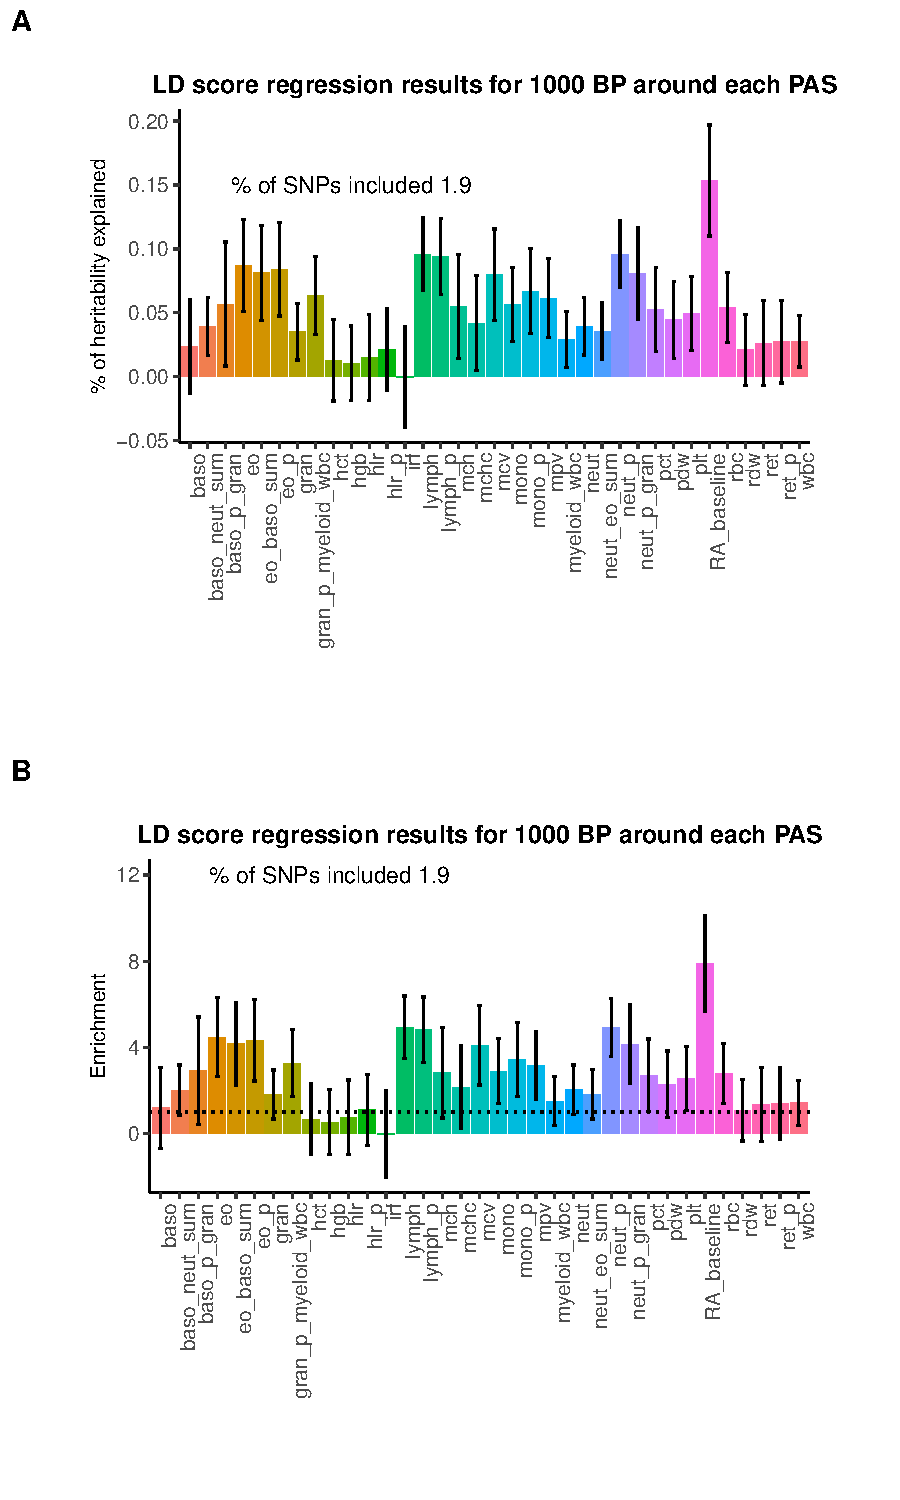
\includegraphics[width=5in]{img/ch02/Fig4_figuresupplement3.pdf}
\caption[LD Score regression enrichment estimates suggest that APA regulation is likely relevant for complex human phenotypes]{\textbf{LD Score regression enrichment estimates suggest that APA regulation is likely relevant for complex human phenotypes} {\bf (A)} Percent of heritability explained by SNPs within 1kbp around each PAS.}
\label{fig:ldregress}
\end{figure}


\begin{figure}[!htb]
 \contcaption{(continued) Error bars represent +/- 1 standard deviation. Blood phenotype statistics published in Astle et el \citep{astle_allelic_2016}. Rheumatoid arthritis statistics were obtained from Okada et al \citep{okada_genetics_2014}. {\bf (B)} Enrichment of heritability explained by SNPs within 1kbp around PAS for the phenotypes analyzed.}
\label{fig:ldregress}
\end{figure}
\clearpage

\begin{figure}[!htb]
\centering
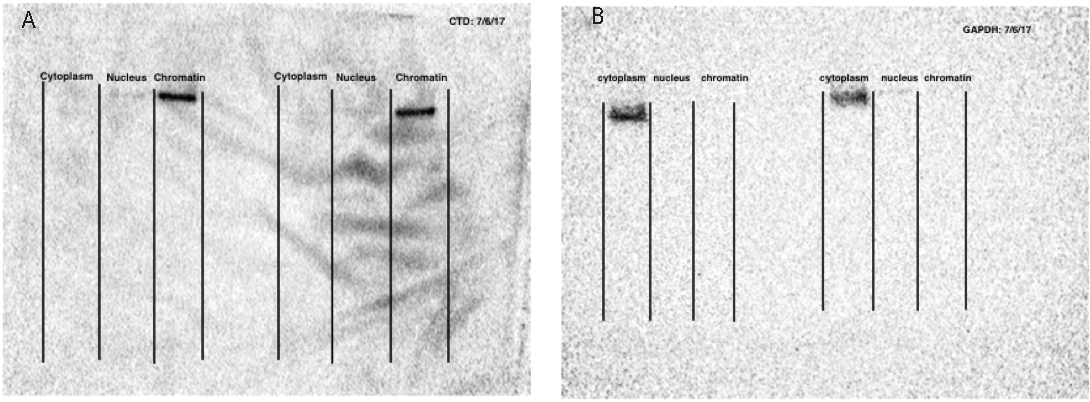
\includegraphics[width=5in]{img/ch02/Fig1_figuresupplement7.pdf}
\caption[Western Blots to demonstrate cell fractionation]{\textbf{Western Blots to demonstrate cell fractionation} {\bf (A)} Western blot against Carboxyl terminal domain of RNA Polymerase II, photo captured at 10 second exposure. Blot is not used for quantification, but to validate cell fractionation. {\bf (B)} Western blot against GAPDH to mark glycolysis in cytoplasm, photo captured at 25 second exposure time. Blot is not used for quantification, but to validate cell fractionation. Figure panels are modeled off Mayer and Churchman 2016, Figure 2 \citep{mayer_genome-wide_2016}}
\label{fig:western}
\end{figure}
\clearpage

\begin{figure}[!htb]
\centering
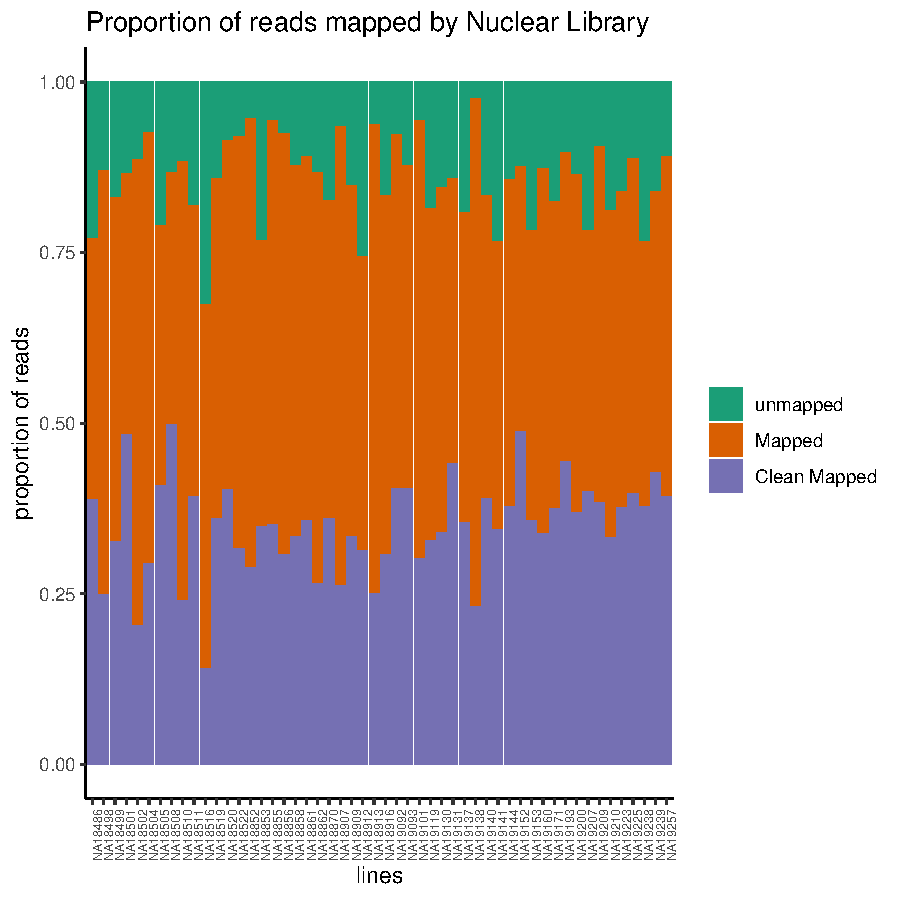
\includegraphics[width=5in]{img/ch02/Fig1_figuresupplement8.pdf}
\caption[3'-Seq read mapping proportions for the nuclear mRNA fraction]{\textbf{3'-Seq read mapping proportions for the nuclear mRNA fraction} Proportion of reads that map to the genome (mapped) and the proportion of final reads used for analysis are cleanly mapped (Clean Mapped) by nuclear mRNA library. Cleanly mapped reads are reads that mapped successfully and passed the filtering for mispriming (MP) as described in the Methods.}
\label{fig:nucMap}
\end{figure}
\clearpage

\begin{figure}[!htb]
\centering
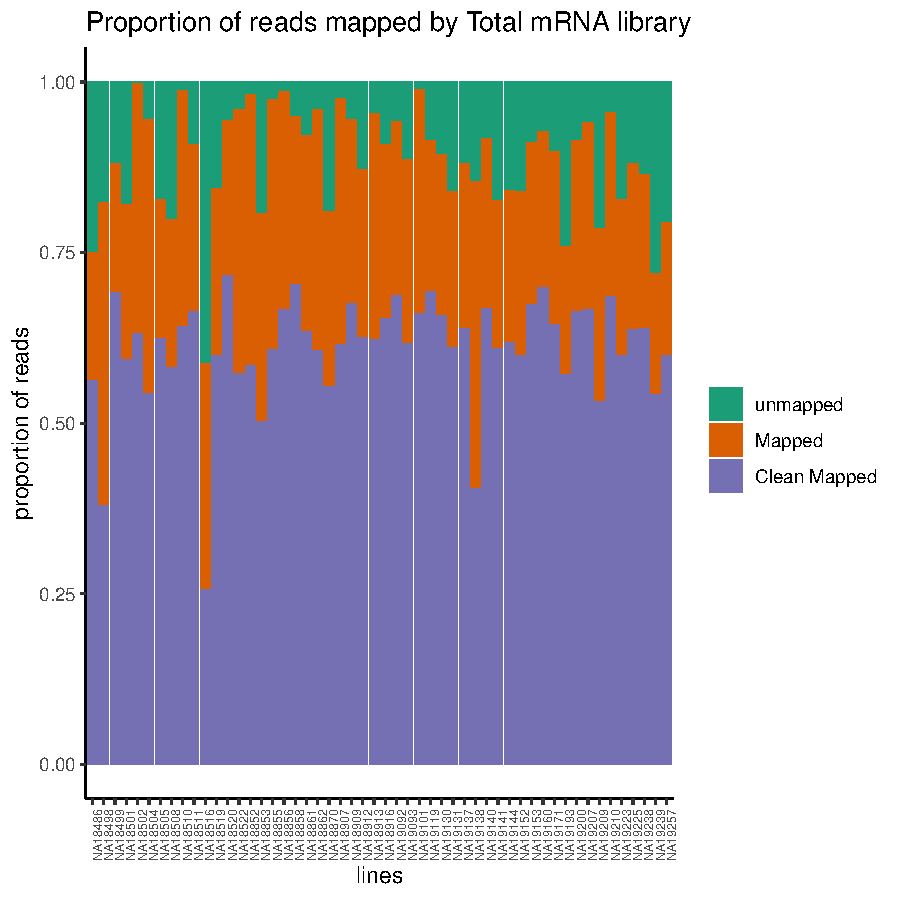
\includegraphics[width=5in]{img/ch02/Fig1_figuresupplement9.pdf}
\caption[3'-Seq read mapping proportions for the total mRNA fraction]{\textbf{3'-Seq read mapping proportions for the total mRNA fraction} Proportion of reads that map to the genome (mapped) and the proportion of final reads used for analysis that are cleanly mapped (Clean Mapped) by total mRNA library. Cleanly mapped reads are reads that mapped successfully and passed the filtering for mispriming (MP) as described in the Methods.}
\label{fig:TotalMap}
\end{figure}
\clearpage

\begin{figure}[!htb]
\centering
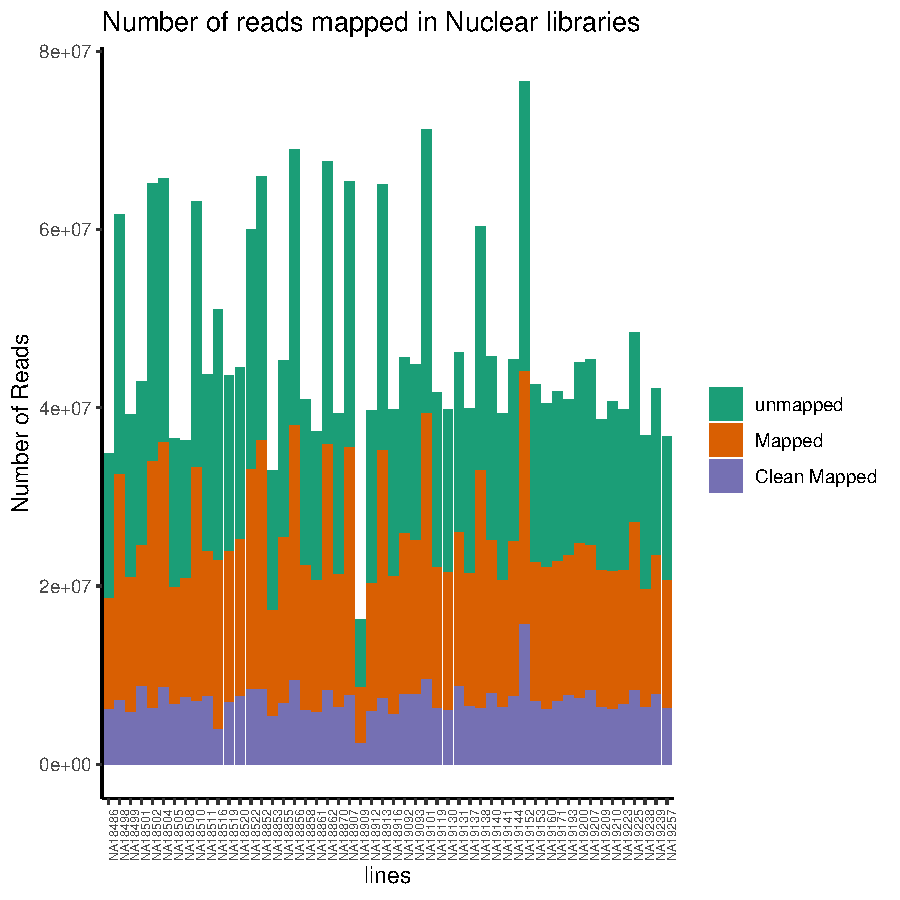
\includegraphics[width=5in]{img/ch02/Fig1_figuresupplement10.pdf}
\caption[3'-Seq reads mapping counts for the nuclear mRNA fraction ]{\textbf{3'-Seq reads mapping counts for the nuclear mRNA fraction } Total number of reads that map to the genome (mapped) and the number of final reads used for analysis that are cleanly mapped (Clean Mapped) by nuclear mRNA library. Cleanly mapped reads are reads that mapped successfully and passed the filtering for mispriming (MP) as described in the Methods.}
\label{fig:NucMapCount}
\end{figure}
\clearpage

\begin{figure}[!htb]
\centering
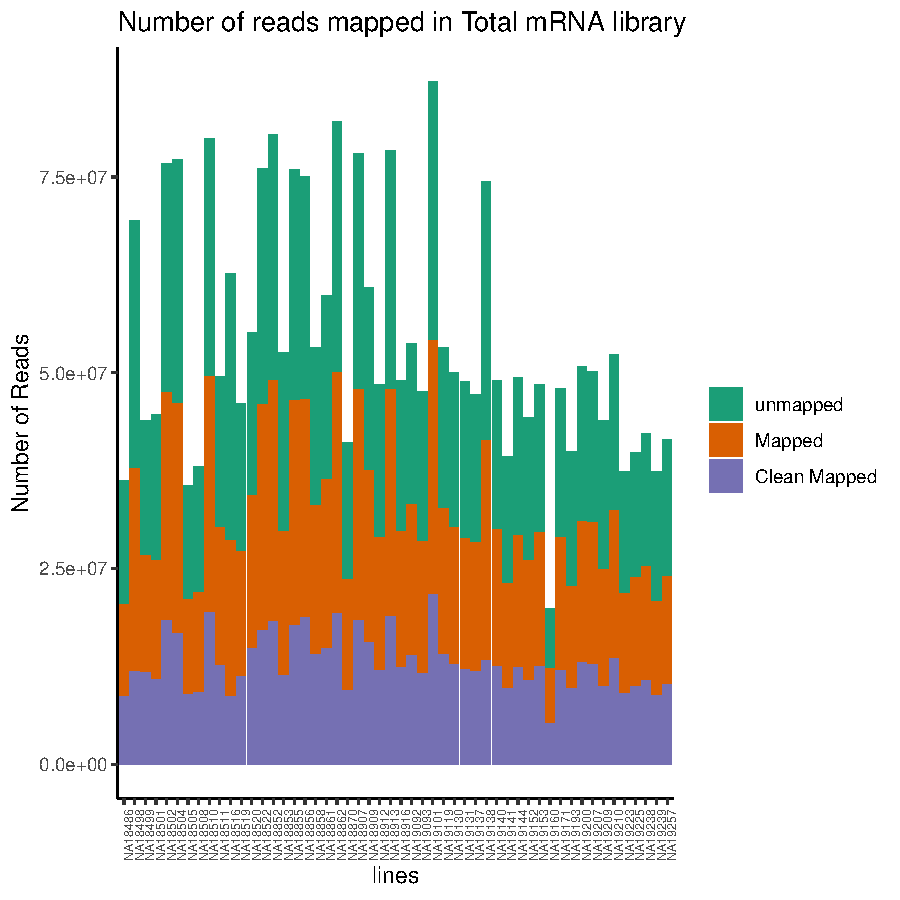
\includegraphics[width=5in]{img/ch02/Fig1_figuresupplement11.pdf}
\caption[3'-Seq reads mapping counts for the total mRNA fraction]{\textbf{3'-Seq reads mapping counts for the total mRNA fraction} Total number of reads that map to the genome (mapped) and the number of final reads used for analysis that are cleanly mapped (Clean Mapped) by total mRNA library. Cleanly mapped reads are reads that mapped successfully and passed the filtering for mispriming (MP) as described in the Methods.}
\label{fig:TotMapCount}
\end{figure}
\clearpage

\begin{figure}[!htb]
\centering
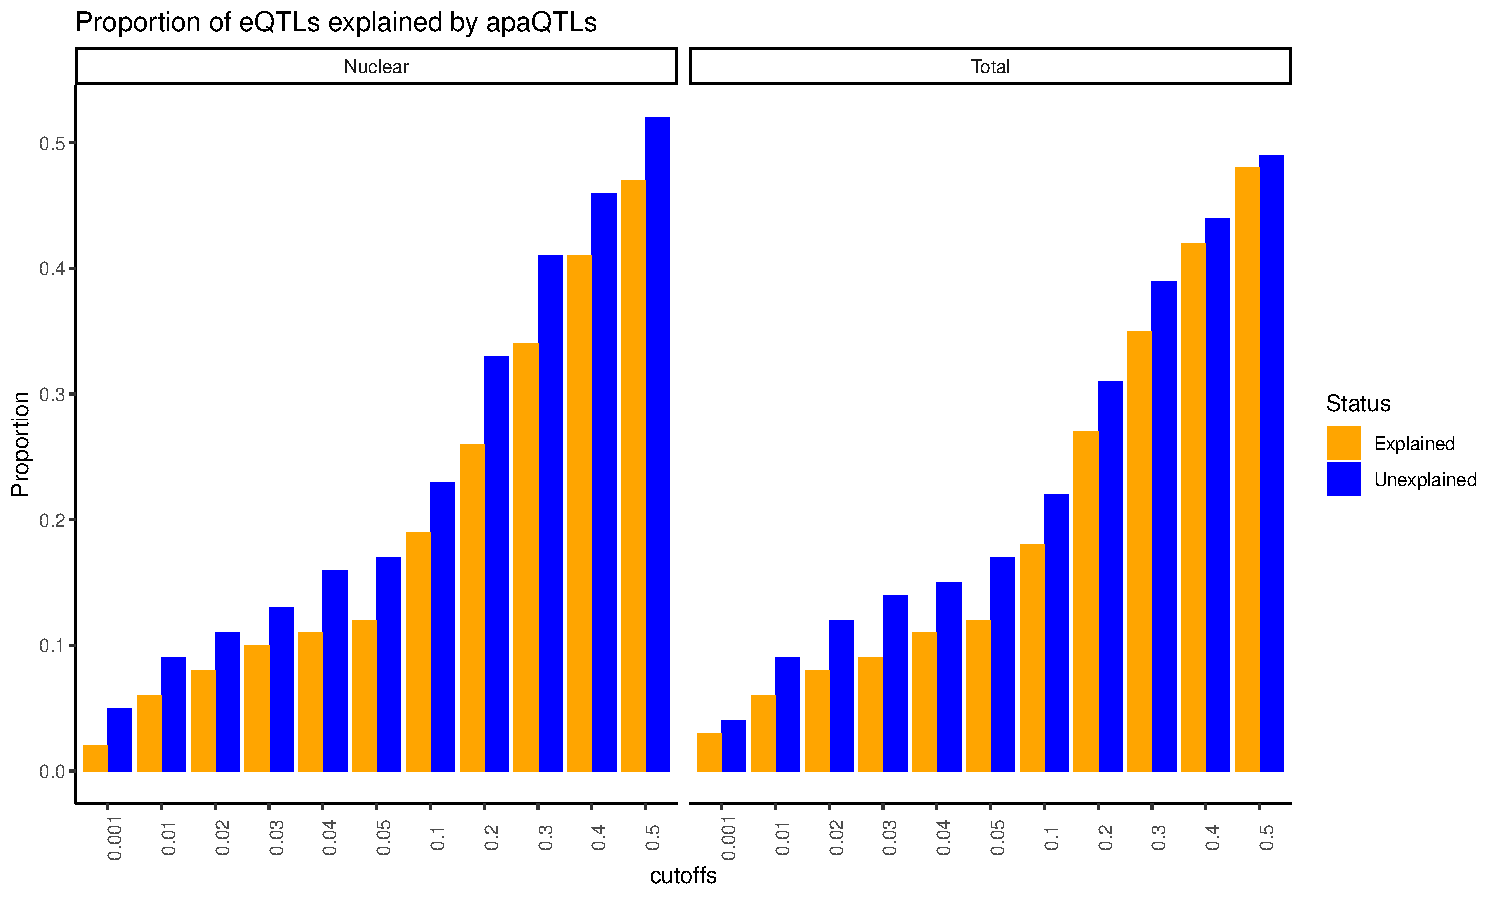
\includegraphics[width=5in]{img/ch02/Fig3_figuresupplement4.pdf}
\caption[Proportion of eQTLs explained by apaQTLs]{\textbf{Proportion of eQTLs explained by apaQTLs} Proportion of eQTLs putatively explained by apaQTLs separated by fraction. Expression QTLs could be explained by apaQTLs identified from both fractions. This observation is robust to apaQTL association p-value cutoffs. We observed that apaQTLs explain a slightly higher proportion of previously unexplained eQTLs. Explained/Unexplained status of each eQTL was determined previously in Li et al. 2016 \citep{li_rna_2016}}
\label{fig:popExp}
\end{figure}
\clearpage

\section{Supplementary file 1}\label{ch02-Supplementary file 1} 

\subsection{3' Sequencing of nuclear mRNA captures mRNA species independent of mRNA decay}\label{ch02-decay}

To ensure that applying 3' Seq on the nuclear mRNA fraction would reflect polyadenylation usage of transcripts that have yet to be subject to decay, we verified that the nuclear mRNA 3' Seq captures features of nascent mRNA species prior to and independent from mRNA decay. To this end, we tested whether the ratio of nuclear to total mRNA 3' Seq reads correlates with measures of RNA decay. We reasoned that if nuclear mRNA captures mRNA species before they are subject to decay, then genes with more nuclear reads relative to total reads should have higher rates of mRNA decay. We used 4sU-seq (30m) data and RNA decay measurements collected in the same panel of lymphoblastoid cell lines (LCLs) as was used in this study as a proxy for mRNA rates of decay. The RNA decay and 4sU data were originally collected and processed in Pai et al. 2012 \citep{pai_contribution_2012} and Li et al. 2016 \citep{li_rna_2016}, respectively. We further used RNA sequencing data collected in the same LCLs as used in this study and details regarding data processing can be found in Li et al. 2016 \citep{li_rna_2016}. 

We computed a score reflecting the nascent transcription rate for each gene as the normalized 4sU count over the sum of the RNA-seq and 4sU counts. This is because 4sU captures nascent mRNA that were metabolically labelled with a modified uridine. After a fixed amount of time (30min in this case), the modified transcripts are sequenced. A positive correlation between 4sU/RNA and nuclear/total 3' Seq across genes suggests that the nuclear 3' Seq captures polyadenylation usage at an earlier stage of the mRNA lifecycle. 

In Li et al 2016, the authors presented a relationship between the same nascent transcription rate and a measure relative mRNA decay rate. They reported a negative correlation between nascent transcription and relative decay, whereby genes with faster nascent transcription also show faster rates of decay. We show a similar relationship between decay rate and our ratio of nuclear 3' Seq to nuclear and total mRNA 3' Seq, suggesting that we are capturing mRNA transcripts prior to mRNA decay in the nuclear fraction. To compute the correlations, we used the summary of the lm function in R. 

Together, these correlations show that nuclear fraction 3' Seq captures information that is not captured in 3' Seq from the total mRNA fraction, and importantly, that the difference is biologically rather than technically driven. Thus, we were able to use 3' Seq data from both nuclear and total mRNA fraction to study how genetic effects regulate APA at multiple stages of the mRNA lifecycle.  In particular, the observed difference between APA in nuclear versus total mRNA fraction supports the notion that if genetic effects were detectable only in the total mRNA fraction, we should suspect that the genetic effect drives variation in post-transcriptional regulation such as decay or export. This assumption is based on the premise that mRNA from the total fraction better reflect mRNA diversity subsequent to decay and export. Because we do not see many examples of genetic effects only identified in the total mRNA fraction, we propose that nearly all genetic effect drive variation in APA co-transcriptionally. 

\begin{figure}
\centering 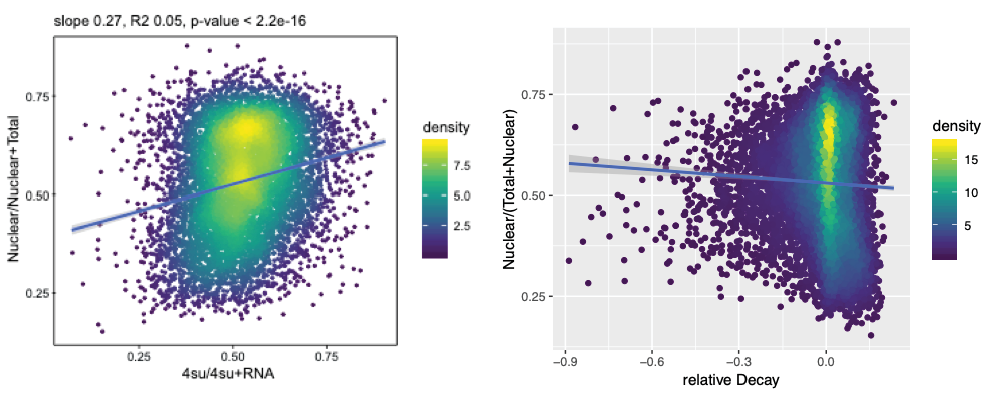
\includegraphics[width=5in]{img/ch02/figureAppendix1.pdf}
\caption[Relationship between 3' Seq and nascent transcription]{ \textbf{Relationship between 3' Seq and nascent transcription}  {\bf (A)}Nuclear 3' Seq captures polyadenylation of nascent transcripts. The ratio of new mRNA to steady-state mRNA (x axis) are plotted against the ratio of 3' Seq reads from the nuclear fraction to 3' Seq reads from the total mRNA fraction (y axis). Slope, $R^{2}$, pvalue from a linear regression.  {\bf (B)} Nuclear 3' Seq captures polyadenylation of mRNA independent of mRNA decay. The relative decay rate of each gene (x axis) are plotted against the ratio of 3' Seq reads from the nuclear fraction to 3' Seq reads from the total mRNA fraction (y axis). Slope, $R^{2}$, pvalue from a linear regression.}
\label{fig:Supplementaryfile1-Fig1}
\end{figure}


\subsection{Intronic polyadenylation in other human tissues}\label{ch02-intronic-other-tissues}

In this study we used LCLs because of the rich molecular phenotyping that has been performed on the same cell lines. By collecting 3' Seq from cell nuclei we uncovered many more intronic PAS than expect. However, we are currently unable to validate whether these PAS are used in other human tissues because we are the first, to the best of our knowledge, to perform 3' Seq on mRNA from isolated nuclei in human cells.

That said, in order to estimate the extent to which intronic PAS we identified in the nuclear fraction are used in other human cell types, we turned to other APA studies that used a similar method to identify whole cell PAS. We reasoned that because total mRNA captures a small fraction of nuclear mRNA, it may be possible to use total mRNA to quantify the extent of intronic alternative polyadenylation in nuclei. For example, we found that 387 intronic PAS that were highly used in LCL nuclear mRNA were also detectable in LCL total mRNA. We can thus ask what fraction of these 387 intronic PAS also show evidence of usage in other cell-types from data collected by other studies on PAS. As baseline, we used 3' Seq usage data collected by Lianoglou et al., which include LCLs and four other cell-types (Breast, Ovary, Testes, Stem Cells). We found that about 10\% of the 387 intronic PAS showed detectable usage in total 3' seq from LCLs collected by the Lianoglou study \citep{lianoglou_ubiquitously_2013}. By contrast, around 5\% of the intronic PAS showed usage in Breast, and Testes. Usage of 3' Seq data from another study performed by Derti and colleagues suggest that nearly 10\% of the 387 PAS showed detectable usage \citep{derti_quantitative_2012}. Thus, these results suggest that there is at most a 2-fold difference in alternative polyadenylation in nuclei in other cell-types. While a 2-fold difference may appear large, we expect different cell-types to use different PAS depending on the specific genes that are expressed. 

\begin{figure}
\centering 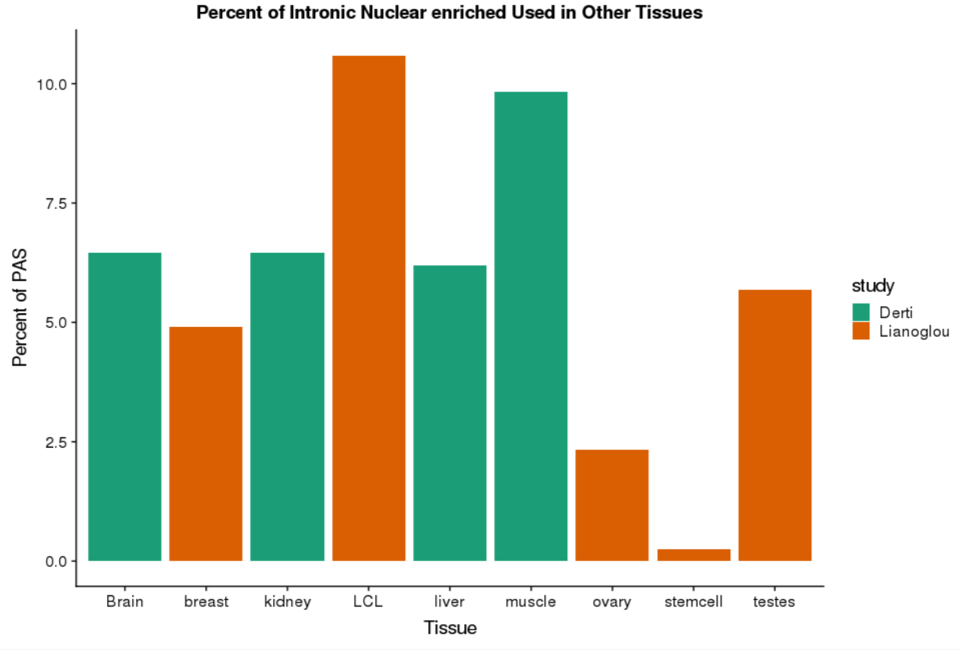
\includegraphics[width=5in]{img/ch02/figureAppendix2.png}
\caption[Intronic PAS Discovered in other tissues]{\textbf{Intronic PAS Discovered in other tissues} Intronic PAS enriched in the nuclear mRNA fraction of LCLs as detected in the total mRNA fraction of other human tissues. Barplot showing the percent of nuclear intronic PAS (of 387) discovered in whole cell 3' Seq from Derti et al. \citep{derti_quantitative_2012}, or Lianoglou et al. \citep{lianoglou_ubiquitously_2013}  Bar for each tissue is colored by study in which the data was collected.}
\label{fig:Supplementaryfile1-Fig2}
\end{figure}



\subsection{RNA binding motifs}\label{ch02-RBPs}

3' UTRs are hotspots for RNA binding protein (RBP) motifs. When bound, RBPs can affect post transcriptional gene regulatory processes such as translation efficiency and nuclear export. We wanted to investigate whether genetic variants can impact APA by affecting binding of RBPs. To do this, we asked whether 3' UTRs with an apaQTL were more likely to be bound by an RBP than expected by chance. We downloaded eCLIP data for 25 RBPs collected by the ENCODE project in human K562 cells. We identified several RBPs enriched for genes with apaQTLs associated with 3' UTR PAS, but the overall enrichments were weak and are unlikely to explain the mechanism that underlie most apaQTLs. We did not see a similar enrichment for genes with intronic PAS apaQTLs. Interestingly, we found that the RNA binding proteins with the strongest enrichments are FUS and SAFB. These are intriguing result given the known function of FUS as a splice factor that guide nuclear export. We next asked if a genetic variant could be identified as an apaQTL due to differentially effects on one isoform but not the others. While we do not expect this to be the case genome wide, we do expect a small number of examples where a QTL could affect binding of an RBP and therefore isoform-specific post-transcriptional gene regulation.  We identified 37 nuclear and 26 total apaQTLs overlapping eCLIP peaks. Of note, two apaQTLs disrupt binding for UPF1 which is a critical factor for nonsense mediated decay. A caveat to this analysis is the cell type specificity of RBP binding. eCLIP data is not available for LCLs. 


\begin{figure}
\centering 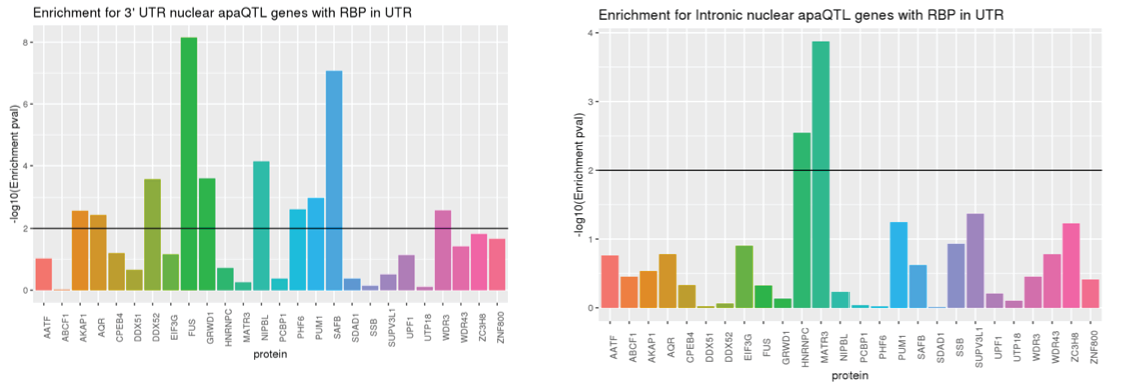
\includegraphics[width=5in]{img/ch02/figureAppendix3.pdf}
\caption[Enrichment for RNA binding in K652 cells]{\textbf{Enrichment for RNA binding in K652 cells}{\bf (A)}Enrichment for K562 cell RBP binding in 3' UTRs of genes with apaQTLs most strongly associated with a PAS in 3' UTRs compared to genes without apaQTL {\bf (B)} Enrichment for K562 cell RBP binding in 3' UTRs of genes with apaQTLs most strongly associated with an intronic PAS compared to genes without apaQTL }
\label{fig:Supplementaryfile1-Fig3}
\end{figure}


\subsection{Correlation between variance in ribosome occupancy and variance in APA }\label{ch02-var-ribo}


Variation in 3' UTR length can drive variation in translation efficiency. We wanted to test if this effect can be seen at the level of inter individual variation without requiring the existence of a QTL. We reasoned that if APA plays a role in modulating translation efficiency, then we would expect a correlation between APA variance and ribosome occupancy variance. When we correlated the variance in usage for the most highly used PAS for each gene, we see a weak but significant positive correlation between APA variance and ribosome occupancy variance (Correlation = 0.15, $p <2.2\times10^{-16}$).   

\begin{figure}
\centering 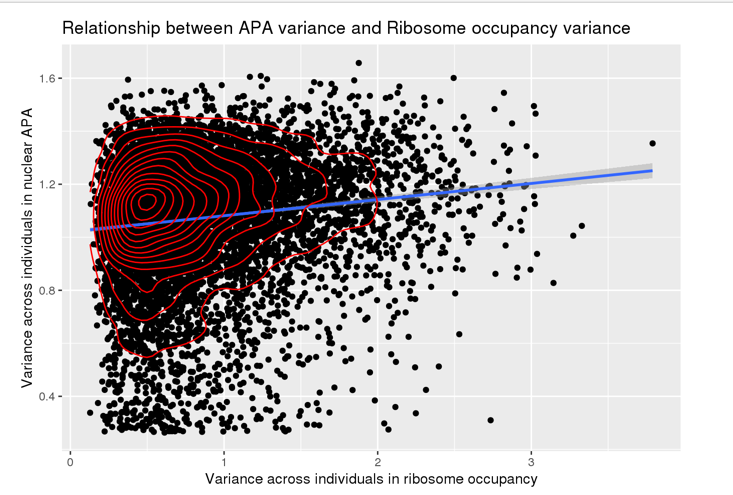
\includegraphics[width=5in]{img/ch02/figureAppendix4.png}
\caption[Variance in APA and Ribosome Occupancy]{\textbf{Variance in APA and Ribosome Occupancy} Individual usage variance of the most highly used PAS in each gene (x axis) correlates with individual variance in ribosome occupancy (y axis) as measured in Li et al 2016.\citep{li_rna_2016}}
\label{ffig:Supplementaryfile1-Fig4}
\end{figure} 


\subsection{Colocalization}\label{ch02-coloc}


In the main text we assert that APA can explain a proportion of the unexplained eQTLs, i.e. chromatin independent eQTLs. We primarily relied on correlation in order to draw this conclusion. However, to strengthen our claim, we used colocalization to ask if apaQTLs might generally be causal for the correlated eQTLs. To quantify the amount of colocalization between our apaQTLs and eQTLs, we used the COLOC package to test whether the apaQTL and eQTL associations share a causal SNP. The COLOC package estimates Bayes Factors for 4 alternative hypotheses. PP0: No association with either trait, PP1: No association with trait 1, PP2: No association with trait 2, PP3: Association with trait 1 and trait 2, two independent SNPs, and PP4: Association with trait 1 and trait 2, one shared SNP. If causal SNPs for an apaQTL and an eQTL is the same SNP, then PP4 is expected to be large > 0.5. One limitation of COLOC is that it is very sensitive to sample size and tend to assign large posterior probability to PP0, PP1, PP2 when either of the QTL mapping suffer from low power. This is because QTL mapping suffer from low power due to very small sample sizes compared to GWASs, for which coloc was designed for. To overcome this limitation, we used the ratio PP4/(PP3+PP4) to assess the colocalization probability instead of PP4/(PP0+PP1+PP2+PP3+PP4). To further increase power in our analysis, we used summary statistics from eQTLs identified on Geuvadis YRI LCL sample (n = 90) and used coloc to find colocalization between the eQTL signal and apaQTLs for the polyadenylation site (PAS) that is the most significant for the same gene. We expect this to be a lower bound for the actual number of colocalized eQTL-apaQTL SNPs because only one PAS for each gene is tested. Overall, we found that 33 genes had both and apaQTL and an eQTL and for which PP3+PP4 from coloc was 0.2 or greater. We found that the vast majority of genes (26, 78.8\%) had a PP4/(PP3+PP4) value greater than 0.5, which indicates that the apaQTL and eQTL are more likely to share a causal SNP than not. Thus, we conclude that most apaQTLs that are determined to be eQTLs are likely to be causal, and further likely explain all the SNP effect on gene expression.


\begin{figure}
\centering 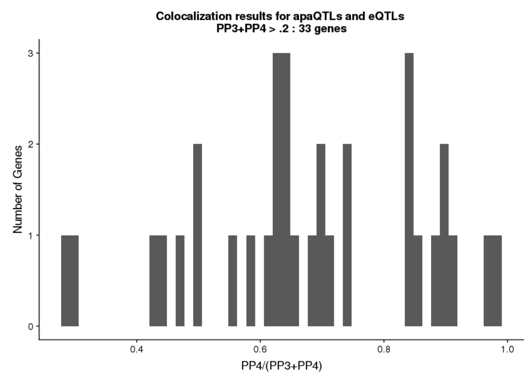
\includegraphics[width=5in]{img/ch02/figureAppendix5.png}
\caption[Colocalization of apaQTLs and eQTLs]{\textbf{Colocalization of apaQTLs and eQTLs} The apaQTL and eQTLs for the large majority of genes that have both are more likely to colocalize than not. Histogram of number of genes with an apaQTL and eQTL for different values of PP4/(PP3 +PP4).}
\label{ffig:Supplementaryfile1-Fig5}
\end{figure} 

\subsection{Evaluating the robustness of our finding to false positives caused by mispriming}\label{ch02-MP-robust}

We took various measures to ensure that misprimed reads are not included in our analysis. For example, we include filters both at the read and PAS level according to previous reports using the same experimental protocol (methods). In order to test if mispriming could still be responsible for the PAS we identified, we have looked at the base composition around our PAS. The results are below with 10 base pairs up and downstream of the PAS (PAS are at position 10 on plot). We have separated PAS based on their location and on whether the PAS is annotated in polyADB. We found a very similar base pair composition for all PAS except for intronic PAS that are unannotated in polyA DB. This suggests there may be some amount of mispriming for intronic PAS that are not annotated in the polyADB. By quantifying the increase in A at nearby position around unannotated intronic PAS relative to annotated intronic PAS, we estimate that up to 20\% of our unannotated intronic PAS may be explained by mispriming. 


\begin{figure}
\centering 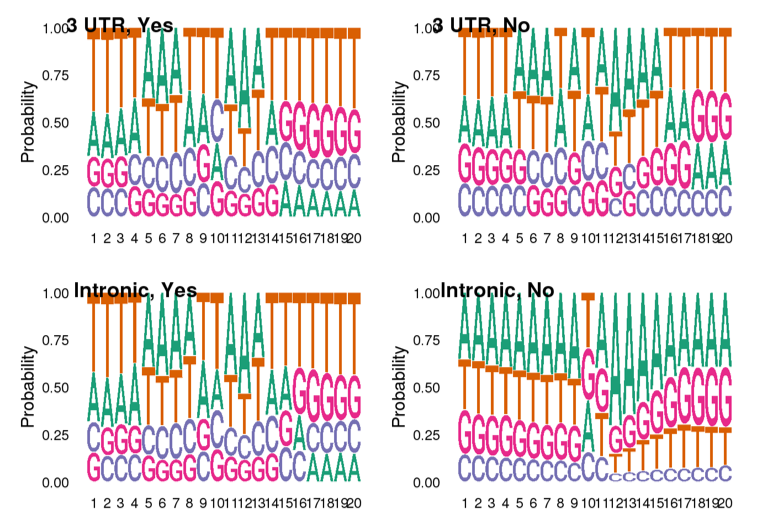
\includegraphics[width=5in]{img/ch02/figureAppendix6.png}
\caption[Base Composition around PAS]{\textbf{Base Composition around PAS} Position weight matrices representing base composition 10 bps upstream and downstream of identified PAS separated by location and presence/absence of site in polyA DB.}
\label{fig:Supplementaryfile1-Fig6}
\end{figure} 


However, we believe that the vast majority of unannotated intronic PAS are likely to be real. To support this view, we found that of the 9,605 unannotated intronic PAS, 24.6\% have a canonical polyadenylation signal site upstream of the PAS. This matched the fraction of intronic PAS that are annotated, and is significantly higher than background (which is about 0.24\%). Furthermore, the location of the canonical polyadenylation signal site relative to the PAS location follows the expected distribution, which is 10-30bp upstream.   


\begin{figure}
\centering 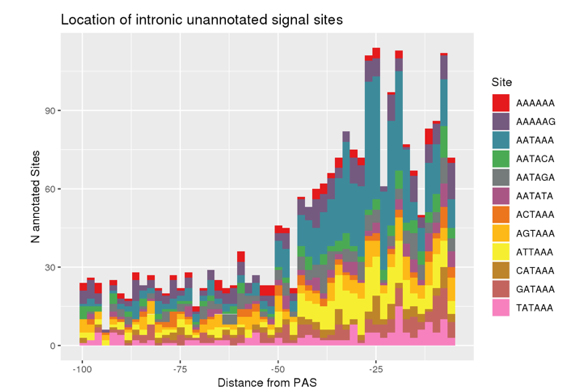
\includegraphics[width=5in]{img/ch02/figureAppendix7.png}
\caption[Signal site distribution for intronic unannotated PAS]{\textbf{Signal site distribution for intronic unannotated PAS} Stacked histogram of polyadenylation signal sites upstream of unannotated intronic PAS. Distribution similar in shape and structure to that in Figure 2.1D. }
\label{fig:Supplementaryfile1-Fig7}
\end{figure} 


While we would argue that a 20\% rate of mispriming is reasonably low, and removing more PAS would lead to many false negatives, we nevertheless decided to rerun our analysis after removing intronic PAS that have not been previously annotated, to make sure that our results are robust to misprimed contaminates. We re-calculated the correlation between intronic effect sizes and eQTL effect sizes and found that the correlation is stronger than when the unannotated PAS are included (349 vs 357). This suggests that mispriming may be increasing noise. 

\begin{figure}
\centering 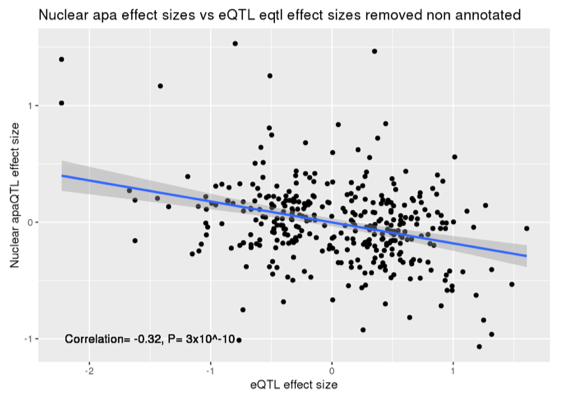
\includegraphics[width=5in]{img/ch02/figureAppendix8.png}
\caption[Figure 2.3A without unannotated intronic PAS]{\textbf{Figure 2.3A without unannotated intronic PAS} Scatter plot of intronic apaQTL effect sizes after removing associations with unannotated intronic PAS plotted against their eQTL effect sizes. Supplemental to Figure 2.3A. }
\label{fig:Supplementaryfile1-Fig8}
\end{figure} 



We also found that the proportion of eQTLs that are significant apaQTLs does not change dramatically (18\% vs 17.3\% of unexplained eQTLs using the 0.05 cutoff).

\begin{figure}
\centering 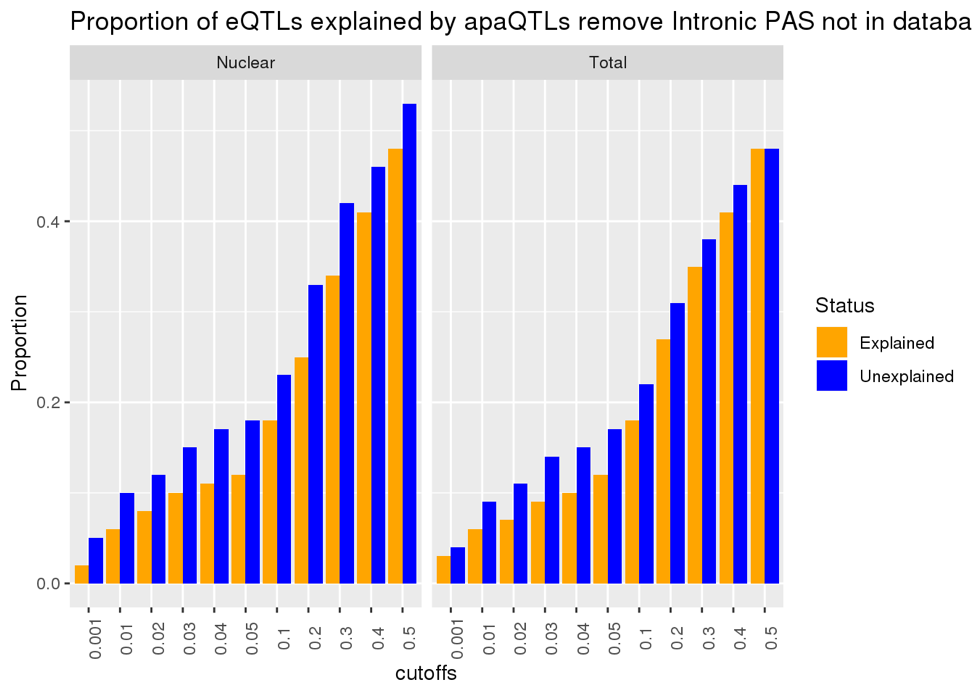
\includegraphics[width=5in]{img/ch02/figureAppendix9.png}
\caption[Proportion eQTL explained without unannotated intronic PAS]{\textbf{Proportion eQTL explained without unannotated intronic PAS} Proportion of putatively explained by apaQTLs separated by fraction after removing associations with unannotated intronic PAS. Expression QTLs could be explained by apaQTLs identified from both fractions. This observation is robust to apaQTL association p-value cutoffs. We observed that apaQTLs explain a slightly higher proportion of previously unexplained eQTLs. Explained/Unexplained status of each eQTL was determined previously in Li et al. 2016.\citep{li_rna_2016}}
\label{fig:Supplementaryfile1-Fig9}
\end{figure} 

Lastly, we found that nearly all apaQTLs that are not eQTLs but are associated with differences in translation and protein expression are not affected by the removal of unannotated intronic PAS (20 vs 25). Together these analyses suggest that even if our set of intronic PAS include some false positives, these PAS do not drive the main conclusions of our work.  



\clearpage
\section{Supplementary Tables}\label{ch02-supplementary-tables}

\begin{table}[!htb]
\caption[Expression Independent eQTLs]{\textbf{Expression Independent eQTLs} 
(see supplementary file associated with this
  dissertation) apaQTL whose lead SNP is nominally associated with protein expression levels but not expression. Table includes p-value and slope for the associated between the lead SNP and nuclear APA usage, gene expression levels, protein expression levels, and ribosome occupancy (as measured using ribo-seq). mRNA, protein and translation data reported in Li et al. 2016\citep{li_rna_2016}.}
\label{tab:ch02-s1}
\end{table}

\begin{table}[!htb]
\caption[Meta Data]{ \textbf{Meta data}  (see supplementary file
  associated with this dissertation) Library information for each Yoruba lymphoblastoid cell line, including sample,
collection, and read information. Column names as described: Sample\_ID: Sample ID, line: YRI Line,fraction: Molecular fraction, batch:3' Sequencing batch, fqlines: number of lines in fastQ file (used to calculate reads),reads: number of sequenced reads, mapped: number of mapped reads,  Mapped\_noMP:number of reads mapped after misprimmed reads are removed, prop\_MappedwithoutMP, proportion of usable reads, Sex: Sex of YRI sample, Wake\_Up: Date up cell line wakeup, Collection: Date of cell collection, count1:cell count measurements ($1x10^{^6}$) , count2:cell count measurements ($1x10^{^6}$), alive1: percent of cells alive calculated with trypan blue stain, alive2:percent of cells alive calculated with trypan blue stain, alive\_avg: average of two percent alive measurements,  undiluted\_avg: average of two cell count measurements ($1x10^{^6}$), Extraction: Date of mRNA extraction, Concentration: RNA concentration ng/ul, ratio260\_280: RNA quality collected from nanodrop, to\_use: amount of RNA input for 3' seq, h20: amount of water used for 3' seq, threeprime\_start: data of library collection, Cq: quantification measurement from qPCR during 3'  seq library preparation, cycles: cycles used for library prep, library\_conc: concentration of 3'  seq library (ng/ul).}
\label{tab:ch02-s2}

\end{table}





% Chapter 03
\chapter{Divergence in alternative polyadenylation contributes to gene regulatory differences between humans and chimpanzees}\label{ch:comp}

\section[Abstract]{Abstract\footnotemark}


Comparative functional genomic studies have shown that differences in gene expression between species can often be explained by corresponding inter-species differences in genetic and epigenetic regulatory mechanisms. In the quest to understand gene regulatory evolution in primates, the role of co-transcriptional regulatory mechanisms, such as alternative polyadenylation \emph{(APA)}, have so far received little attention. To begin addressing this gap, we studied APA in lymphoblastoid cell lines \emph{(LCLs)} from six humans and six chimpanzees, and comparatively estimated polyadenylation site \emph{(PAS)} usage for 44,432 PAS in 9,518 genes. While APA is largely conserved in humans and chimpanzees, we identified 1,705 genes with significantly different PAS usage (FDR of 0.05) between the two species. We found that genes with divergent APA patterns are enriched among differentially expressed genes, as well as among genes that show differences in protein translation between species. In particular, differences in APA between humans and chimpanzees can explain a subset of observed inter-species protein expression differences that do not display corresponding expression differences at the transcript level. Finally, we focused on genes that have a dominant PAS, meaning the gene has a PAS that is used more often than all others for the same gene. Dominant PAS are highly conserved, and inter-species differences in dominant PAS are particularly enriched for genes that also show expression differences between the species. This study establishes APA as another key mechanism underlying the genetic regulation of transcript and protein expression levels in primates.


\footnotetext{Citation for chapter: Mittleman BE, Pott S, Warland S, Barr K, Cuevas C, and Gilad Y. Divergence in alternative polyadenylation contributes to gene regulatory differences between humans and chimpanzees. Manuscript in Prep}

\section{Introduction}\label{ch03-introduction}


Humans and our close primate relatives exhibit a striking array of phenotypic diversity despite sharing homologous proteins with nearly identical amino acid sequences. Understanding how this diversity is propagated from genomic sequence to mRNA and protein necessitates an understanding of the regulatory mechanisms that occur before, during, and after transcription.  Studying gene regulatory features in humans and other primates has long provided opportunities to understand genome evolution and function. For example, studies comparing patterns of epigenetic marks in primates have \citep{banovich_methylation_2014, cain_gene_2011,McVicker2013, pai_genome-wide_2011}. Although many studies have focused on interspecies differences in the regulation of gene expression, fewer studies have addressed isoform-level variation, which contributes to differences in mRNA, translation, and protein levels between species.  

The main mechanisms that contribute to mRNA isoform diversity are alternative splicing and alternative polyadenylation \emph{(APA)}. Alternative splicing produces different combinations of coding sequences in mature mRNA and protein. APA occurs at genes that have more than one polyadenylation site \emph{(PAS)} and can result in mRNAs with different coding sequences or variable 3' UTR lengths. Like alternative splicing, APA that occurs within the gene body can affect protein sequence and function \citep{lee_widespread_2018, pan_intronic_2006, sandberg_proliferating_2008, tian_alternative_2017, vasudevan_non-stop_2002, yao_genomewide_2018}. APA that occurs outside of the coding sequence, in the 3' UTRs, can lead to differential inclusion of protein-binding motifs that can affect translational efficiency, mRNA stability, and mRNA localization  \citep{mayr_regulation_2017, tian_alternative_2017}. Yet, despite its potential to produce tremendous variation in mRNA and protein regulation, few studies have explored the contribution of APA to regulatory divergence between species. Indeed, our current understanding of APA conservation in mammals comes from few comparative studies of humans and rodents \citep{ara_conservation_2006, wang_compendium_2018}. However, these studies used sequence conservation rather than direct measurements of PAS usage to characterize APA \citep{wang_compendium_2018}. Thus, it remains possible that many mammalian PAS are functionally divergent despite having similar sequences. 

To gain insight into APA conservation between human and chimpanzees and understand how differences in APA contribute to gene regulation, we performed 3' sequencing (3' Seq) of mRNA isolated from nuclei collected from human and chimpanzee LCLs. We integrated PAS usage measurements with RNA-sequencing data collected from the same cell lines to understand the relationship between APA and gene expression. Finally, we used ribosome profiling and protein measurements previously collected in the same panel of human and chimpanzee LCLs to explore the effects of APA on protein levels \citep{khan_primate_2013, wang_post-translational_2018}, reasoning that an understanding of how APA isoform usage varies among primates could help to explain why some human and chimpanzee genes are differentially expressed at the mRNA or protein levels, but not both.

\section{Results}

\subsection{Describing alternative polyadenylation in human and chimpanzee LCLs }\label{descSpec}

We performed 3' sequencing (3' Seq) of mRNA from 6 human and 6 chimpanzee lymphoblastoid cell lines \emph{(LCLs)}, which we have previously used to study a variety of other functional genomic phenotypes \citep{cain_gene_2011, khan_primate_2013, wang_post-translational_2018, zhou_epigenetic_2014}. We collected mRNA separately from whole cells and isolated nuclei. The two cellular fractions serve as biological replicates, which we used to examine the quality of our data (Methods). In addition, by collecting data from isolated nuclei, we were able to capture polyadenylated transcripts before they became undetectable due to other regulatory processes, such as isoform-specific decay \cite{mittleman_alternative_2020}.  

We mapped human 3' Seq reads to the GRCh38 reference genome and chimpanzee 3' Seq reads to the panTro6 reference genome \citep{chimpanzee_sequencing_and_analysis_consortium_initial_2005, schneider_evaluation_2017}  (Methods). 3' Seq relies on a poly(dT) primer to target the poly(A) tail of mRNA molecules; however, it can also mis-prime by binding a sequence of genomic adenines. To account for mis-priming of off-target genomic sequences we removed reads that mapped to genomic regions containing $\geq70\%$ adenine or 6 consecutive adenine bases in the 10 bp directly upstream of the mapped location  \citep{mittleman_alternative_2020, sheppard_accurate_2013, tian_large-scale_2005} (Methods). In addition, we treated all ambiguous nucleotide positions as adenines to ensure that differences in reference genome quality did not bias the detection of polyadenylation sites \emph{(PAS)} or mis-priming events (Methods). As expected, the filtered aligned sequences, merged by species, were enriched at transcription end sites \emph{(TES)} and showed a similar distribution along orthologous 3' UTRs (Methods, Supplementary Figure \ref{fig:ch03-deeptools}). Next, we used a custom peak calling method to ascertain PAS in humans and chimpanzees separately (Methods) To compare PAS usage across species, we needed to identify the orthologous genomic regions of all PAS in our dataset, regardless of the species in which they were originally annotated. As we were unable to confidently identify orthologous PAS at base pair resolution (inferring synteny at base pair resolution in non-coding regions is challenging\citep{broad_institute_sequencing_platform_and_whole_genome_assembly_team_high-resolution_2011}),  we extended each PAS by 100 bp upstream and downstream. We then used a reciprocal liftover pipeline to obtain an inclusive set of PAS regions with which we could confidently compare PAS usage between species (Methods). 


To quantify PAS usage, we first assigned each PAS to a gene using the hg38 RefSeq annotation \citep{pruitt_ncbi_2005}. We then computed usage for each PAS in each individual as the fraction of reads mapping to one PAS over the total number of reads mapping to any PAS for the same gene (Supplementary Figure \ref{fig:ch03-UsageCalc}). We excluded PAS in lowly expressed genes or with less than 5\% usage, as measurements from sparse data are highly susceptible to random error (Methods). We observed a strong correlation between PAS usage in mRNA from the nuclear and total cell fractions in all but one cell line (human NA18499; Supplementary Figure \ref{fig:ch03-removeInd}). We re-identified PAS after removing all data from NA18499 and re-quantified PAS usage using nuclear 3' Seq data from 5 human and 6 chimpanzee LCLs. Using this analysis pipeline we identified a total of 44,432 PAS in 9,518 genes, which we used for all downstream analyses. On a genome-wide scale, we found that mean PAS usage is highly correlated between species (Pearson's Correlation, 0.9, $p<2.2x10^{-16}$, Supplementary Figure \ref{fig:ch03-UsageCorr}). However, as expected, 41.8\% of the variation in PAS usage (as explained by the top principal component of the data) is highly correlated with species (Pearson's correlation 0.99, $p =2.95x10^{-8}$, Supplementary Figure \ref{fig:ch03-PCAthreeprime}). 


We used a number of analyses to ensure our ability to detect PAS was not biased by gene expression level or species. If our ability to detect PAS was biased by gene expression, we would expect a positive correlation between gene expression level and the number of PAS we detected. In our data, the number of PAS per gene is negatively correlated with gene expression in both species (Supplementary Figure \ref{fig:ch03-PASexp}, Human: Pearson's correlation -0.17, $p <2.2x10^{-16}$, Chimpanzee: Pearson's correlation -0.19, $p<2.2x10^{-16}$). If our ability to detect PAS was biased by species, we would expect to identify more PAS per gene in one species over the other. This is neither the case genome-wide nor when we test each gene independently. We identified, on average, 3.87 PAS per gene in humans and 3.46 PAS per gene in chimpanzees. On average, per gene, the number of PAS in human minus the number of PAS in chimpanzee is 0.39 with a median value of 0 (Supplementary Figure \ref{fig:ch03-SpecPASnum}. Moreover, as expected, the physical distribution of PAS across genes is conserved, with the majority of PAS located in 3' UTRs (17,688 (40.1\%) in chimpanzee and 17,620 (40.0\%) in human) and a considerable proportion located in introns (14,095 (31.9\%) in chimpanzee and 14,119 (32.0\%) in human) (Figure \ref{fig:Ch3fig1}A).

To assess sequence conservation in PAS regions, we downloaded phyloP scores computed over 100 vertebrate genomes from the UCSC Genome Browser and calculated mean phyloP scores in PAS regions. Higher mean phyloP scores corresponds to regions of higher sequence conservation, and thus, slower evolution \citep{pollard_detection_2010}. Overall, sequence elements at PAS are more conserved than surrounding regions (Figure \ref{fig:Ch3fig1}B, Wilcoxon rank sum test, $p<2.2x10^{-16}$). This pattern holds independently for PAS in all genic locations other than introns (Supplementary Figure \ref{fig:ch03-phylopLoc}). 



We identified 302 and 357 human- and chimpanzee-specific PAS, respectively (Methods). It has been previously shown that most PAS are directly preceded by one of 12 annotated sequence motifs that recruit cleavage and polyadenylation machinery to mRNA molecules as they are transcribed \citep{beaudoing_patterns_2000}. We asked if creation or disruption of a signal site motif could be responsible for species-specific PAS by  mapping  signal site motifs in both human and chimpanzee for each PAS region. Although human and chimpanzee PAS regions are equally likely to contain each of the 12 annotated signal sites (Figure \ref{fig:Ch3fig1}C), only the top two most commonly used motifs, AATAAA and ATTAAA, are associated with increased PAS usage (Supplementary Figure \ref{fig:ch03-SignalUsage}). Thus, we considered only the presence or absence of these two motifs in subsequent analyses. Of the 302 human-specific PAS, 14 have human-specific signal sites and 6 have chimpanzee-specific signal sites. Of the 357 chimpanzee-specific PAS, 24 have a chimpanzee-specific signal site and 6 have a human-specific signal site. These numbers are small; still, species-specific signal sites are more abundant than expected by chance among species-specific PAS in human (5.7X, hypergeometric test, $p=2.30x10^{-7}$) and in chimpanzee (8.3X, hypergeometric test, $p=3.2x10^{-15}$), suggesting that signal site changes can explain a subset of differences in PAS usage. For example, we identified a chimpanzee-specific PAS about 1 kb upstream of a PAS used in both species in the 3' UTR of \emph{MAN2B2}. The ancestral signal site conserved in chimpanzee is AATAAA; however, there has been a T to C transition in the human lineage \citep{blanchette_aligning_2004} (\ref{fig:ch03-exChimpspec}). This transition is likely responsible for the loss of PAS in humans.


 
\begin{figure}
\centering
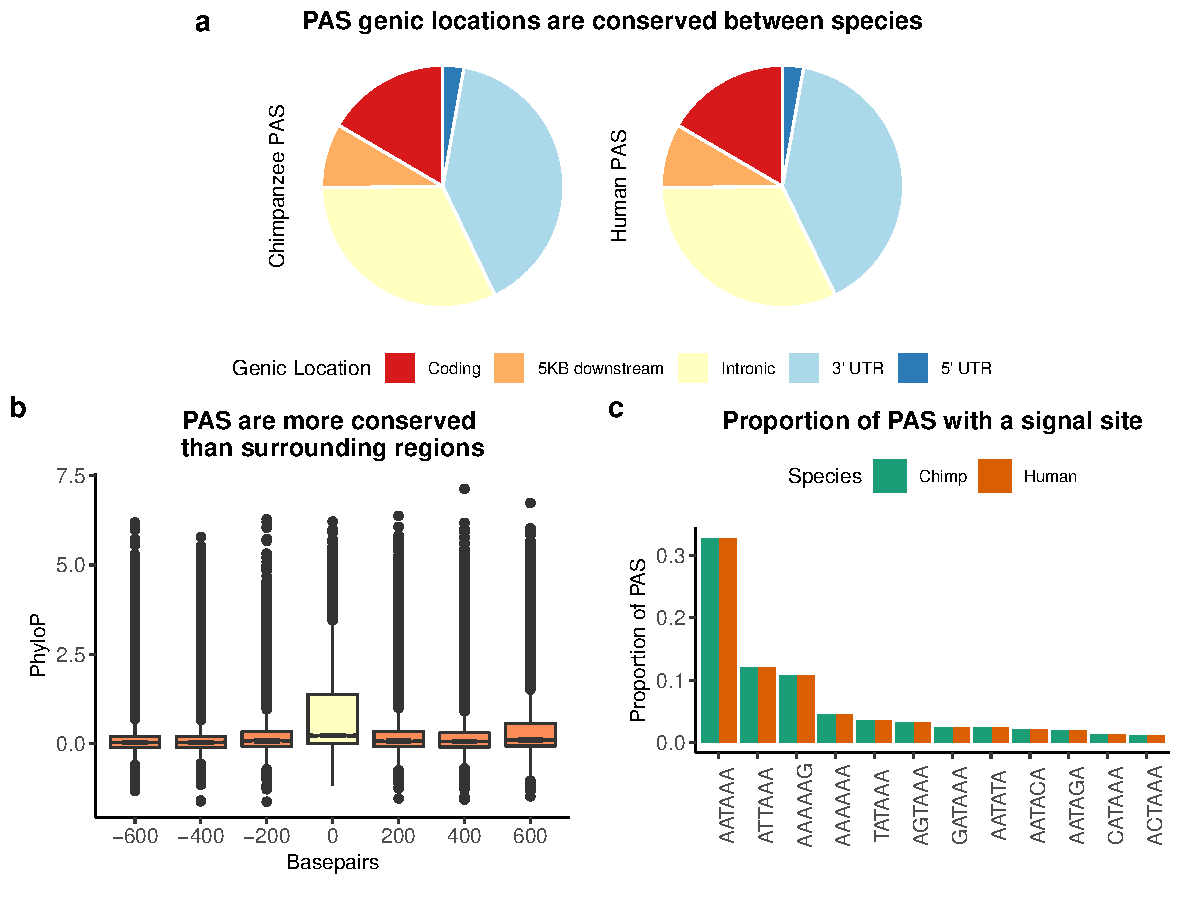
\includegraphics[width=5in]{img/ch03/fig1.pdf}
\caption[Sequence conservation of PAS between humans and chimpanzees]{\textbf{Sequence conservation of PAS between humans and chimpanzees} \small {\bf (A)} Genic locations for 44,074 PAS identified in chimpanzee (left) and 44,130 PAS identified in human (right). {\bf (B)} Mean PhyloP scores for PAS regions (yellow) as well as three 200bp regions upstream and downstream (orange) {\bf (C)} Proportion of human and chimpanzee PAS regions with each of the 12 annotated signal site motifs from Beudoing \emph{et al.}\citep{beaudoing_patterns_2000}} 
\label{fig:Ch3fig1}
\end{figure}
 
 
\subsection{Characterizing inter-species differences in PAS usage}\label{diffHC}

While a few hundred PAS are species-specific, the majority of PAS (98.5\%) were identified in both species. We thus sought to characterize quantitative differences in alternative polyadenylation (APA) patterns between human and chimpanzee by estimating the difference in usage of individual PAS in each species. To do so, we used the leafcutter differential splicing tool \citep{li_annotation-free_2018}, which allowed us to tests for differences in normalized PAS usage fractions while accounting for gene structure (Methods). Using this approach, at an FDR of 5\% we identified 2,342 PAS (in 1,705 genes) whose usage differs by 20\% or more between the species (Figure \ref{fig:Ch3fig2}A). We applied an arbitrary effect size cutoff to focus on larger inter-species differences, which are more likely to have functional consequences. The list of all PAS whose usage differs between the species, regardless of the effect size, is available in Supplemental Table \ref{tab:ch03-s1}. 



 \begin{figure}
\centering
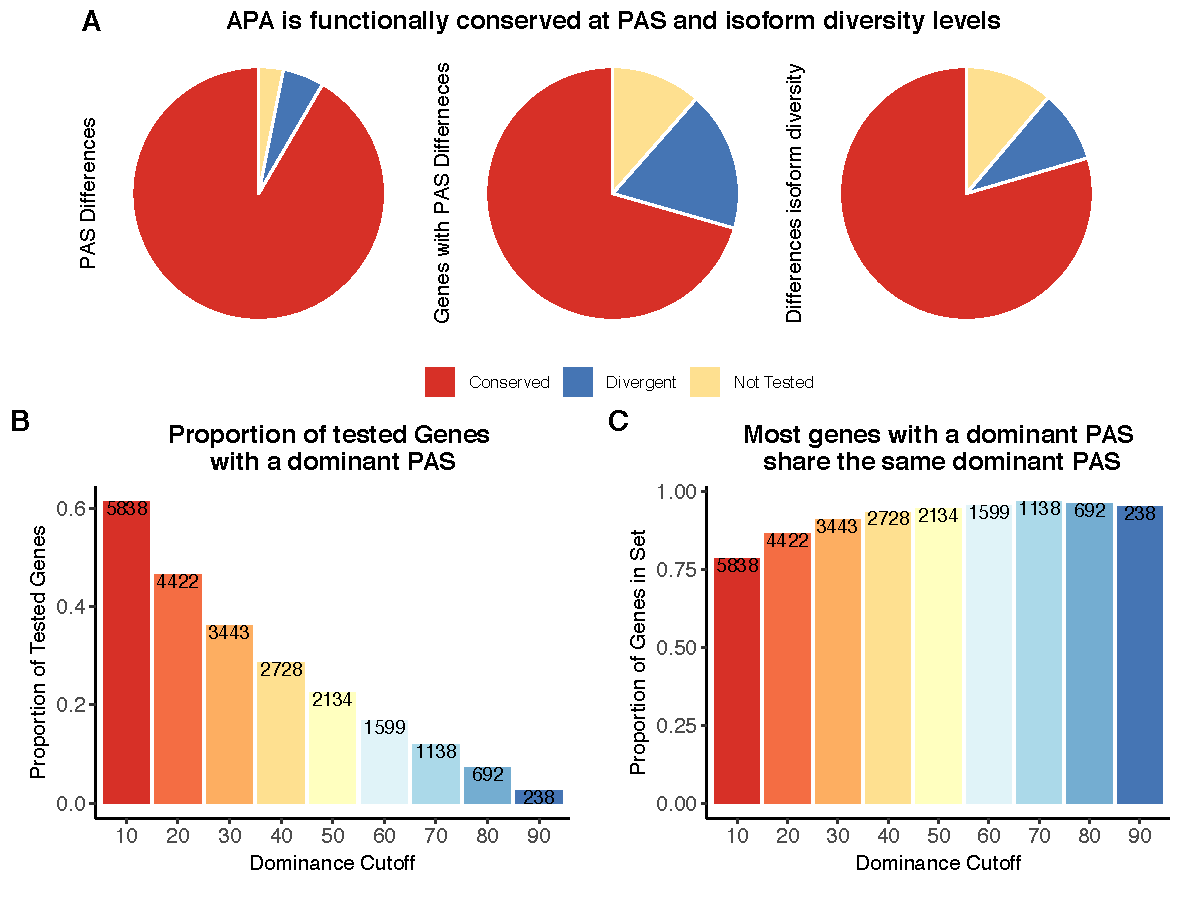
\includegraphics[width=5in]{img/ch03/fig2.pdf}
\caption[APA is functionally conserved between humans and chimpanzees]{\textbf{APA is functionally conserved between humans and chimpanzees.} \small {\bf (A)} Proportion of PAS and genes differentially used at PAS and isoform diversity level. (left) Divergent PAS are the 2,342 PAS differentially used at 5\% FDR. Conserved are the PAS not differentially used at 5\% FDR. Not tested PAS were removed from analysis by leafcutter tool. (middle) PAS level differentially used PAS reported at the gene level. Divergent genes are the 1,705 genes with PAS differentially used at 5\% FDR. Conserved genes are the genes with no PAS differentially used at 5\% FDR.  (right) Divergent genes are the 881 genes with differences in isoform diversity between species at a 5\% FDR. Conserved gene are genes without differences in isoform diversity. Genes with one PAS were not tested. {\bf (B)}  Proportion of tested genes with a dominant PAS in either species according to a range of cutoffs. Number of genes are reported in bars. {\bf (C)} Proportion of the number of the number of genes with a dominant in either species that share the top used PAS according to each dominance cutoff. Number of genes with a dominant PAS is either species are reported in bars.} 
\label{fig:Ch3fig2}
\end{figure}



To better understand the mechanisms that underlie inter-species differences in PAS usage, and the potential functional impact of such differences, we considered the APA data in different contexts. First, we noticed that the spatial distribution of differentially used PAS reflects the distribution of all PAS, namely differentially used PAS are most often located in 3' UTRs, followed by introns (Supplementary Figure \ref{fig:ch03-dPAS}). Within the 3' UTR, however, differentially used PAS are more frequently the first ones compared with PAS that are used similarly in the two species (Supplementary Figure \ref{fig:ch03-whichUTR}, difference in proportion test, $p=0.0015$). This pattern is intriguing, because changes in the usage of the first PAS in the 3' UTR may have the largest overall impact on the transcript length, and hence potentially the largest functional impact as well. However, it is also possible that we are more likely to detect differences in usage in the first PAS in the 3' UTR because this site is transcribed earlier, and our estimate of usage is relative to all other sites in each gene. 

We therefore sought evidence that differences in PAS usage may have functional consequences. In a previous study, we identified genetic variants associated with variation in PAS usage \emph{(apaQTLs)} in a panel of 52 human LCLs \citep{mittleman_alternative_2020}. We found that genes with inter-species differences in PAS usage are highly enriched for apaQTLs (160, empirical p-value based on 10,000 permutations $p=0.001$, Supplementary Figure \ref{fig:ch03-dPASQTL}). This observation indicates that inter-species differences in APA usage can often be found in genes whose regulation varies also at the population level, generally suggesting relaxation of evolutionary constraint on the regulation of such genes. We next considered sequence divergence at PAS by obtaining phyloP scores for all PAS flanking regions (200 bp, as explained above). If many changes in PAS usage are genetically controlled, we expect genomic regions of differentially used PAS to be less conserved than regions flanking PAS sites that have similar usage. Indeed, differentially used sites are enriched for regions with negative mean phyloP scores (hypergeometric test, $p=0.02$). This observation indicates that sequence divergence is often associated with differences in PAS usage, and that the majority of PAS usage in humans and chimpanzees may be generally conserved due to evolutionary constraint. 


We next asked, more specifically, if signal site changes are likely to lead to differences in PAS usage. We addressed this question by performing two analyses. First, we focused on the 82 differentially used PAS with a signal site that is annotated in only one of the species. We found that the presence of a species-specific signal site is associated with increased PAS usage, as might be expected (human enrichment 3.82X, hypergeometric $p=1.37x10^{-10}$, chimpanzee enrichment 3.02X, hypergeometric $p=3.91x10^{-8}$). Second, we considered the presence of G/U-rich elements, which are known signals to the molecular machinery for polyadenylation \citep{colgan_mechanism_1997}. Specifically, we considered the proportion of uracil bases in the PAS regions. Despite a high correlation in overall uracil content in both species (Pearson's correlation 0.99, $p<2.2x10^{-16}$), the usage of PAS with greater uracil density in one species are more likely than expected by chance to be upregulated in that species (Chimpanzee 1.04X enrichment, hypergeometric test $p=0.03$, Human 1.06X enrichment, hypergeometric test $p=0.03$). Though species-specific signal sites explain a modest proportion of inter-species differences in PAS usage, these cases demonstrate the link between sequence evolution and conservation of PAS usage between species. 


\subsection{The relationship between differences in alternative polyadenylation and gene expression}\label{dAPADE}

Our analysis to this point indicates that inter-species differences in PAS usage are often genetically controlled, but generally we have not found strong evidence that they are functionally important. We explored this further by considering the APA data in the context of gene expression data that we collected from the same 6 human and 6 chimpanzee LCLs (see Methods for data collection procedures and low-level analysis of the RNA-seq data). We found no meaningful correlation between inter-species differences in gene expression levels and changes in polyadenylation site usage \emph{($\Delta PAU$)} in 7,462 genes for which we had both types of data (Pearson's correlation = -0.06, $p=3.1x10^{-7}$, Figure \ref{fig:Ch3fig3}A). We then separately considered the data for the 3' UTR and intronic PAS, because we previously found a different relationship between PAS usage in these genic regions and gene expression levels \citep{mittleman_alternative_2020}. Indeed, we found that inter-species differences in the usage of intronic and 3' UTR PAS correlate with differences in expression effect between the species at an equal magnitude, but in opposite directions (Figure \ref{fig:Ch3fig3}B). Increased usage of intronic sites is correlated with increased expression levels, while increased usage of 3' UTR sites is correlated with decreased expression. 

We focused on 3,796 genes that were classified as differentially expressed between humans and chimpanzees at 5\% FDR (Methods). We found that genes with at least one differentially used PAS between the species are more likely to be classified as differentially expressed than expected by chance (610 genes, 1.12X enrichment, hypergeometric test, $p=3.18x10^{-5}$). Examining the subset of 610 genes, we observed a modest but significant negative correlation between differential expression effect size and $\Delta PAU$ when we considered all PAS (Pearson's correlation= -0.15, $p=0.0023$,Figure \ref{fig:Ch3fig3}C). Separating the analysis by PAS genic location revealed, again, an opposite direction of the correlation between gene expression and the usage of either 3' UTR or intronic PAS (Figure \ref{fig:Ch3fig3}D). These observations are consistent when we use PAS data based on 3' Seq data from whole cells instead of from the nuclear fractions, suggesting that the observed relationship is not due to nuclear export failure (Supplementary Figure \ref{fig:ch03-totalDPASDE}, Methods). 

To provide possible mechanistic insight into the relationship between PAS usage and gene expression, we identified AU-rich elements in 3' UTRs in both human and chimpanzee. AU-rich elements in 3' UTRs have been linked to destabilization of mRNA transcripts and translation repression \citep{floor_tunable_2016-1,moore_physiological_2014,siegel_massively_2020}. We found that the 3' UTRs of genes that show an inter-species difference in 3' UTR PAS usage have a higher number (Wilcoxon test, $p < 10^{-16}$) and density (Wilcoxon test, $p < 10^{-16}$) of AU-rich elements compared with genes in which the 3' UTR PAS is similarly used in the two species. 



\begin{figure}
\centering
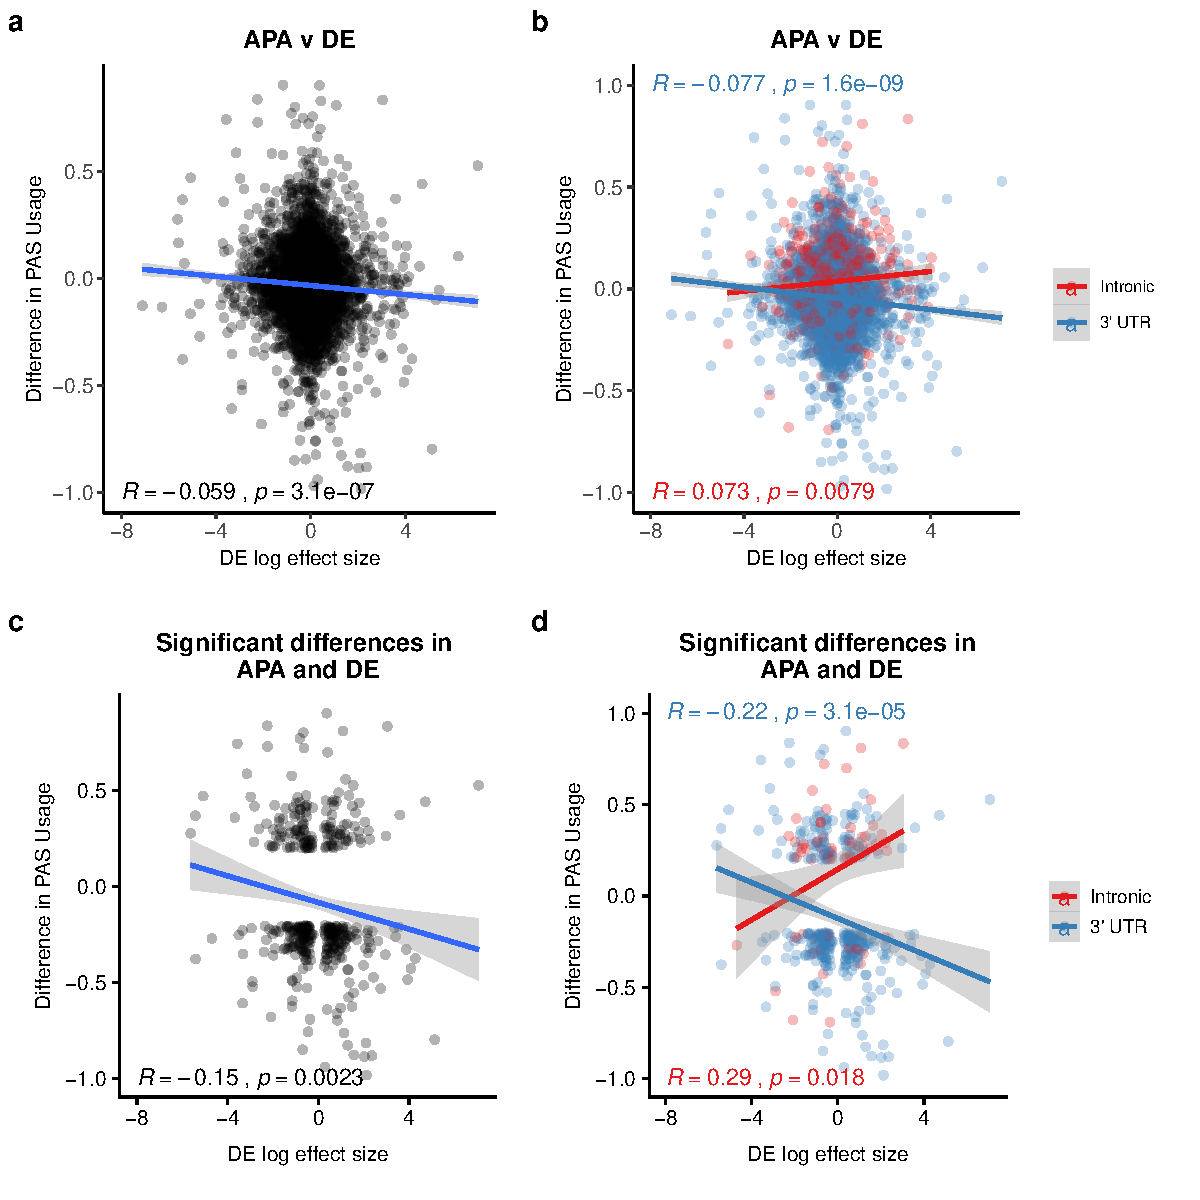
\includegraphics[width=5in]{img/ch03/fig3.pdf}
\caption[PAS usage differences for intronic and 3' UTR PAS correlate with DE effect sizes at similar magnitudes but in opposite directions]{\textbf{PAS usage differences for intronic and 3' UTR PAS correlate with DE effect sizes at similar magnitudes but in opposite directions} \small {\bf (A)} $\Delta PAU$ for top intronic or 3' UTR PAS per gene (Methods) plotted against differential effect size from differential expression analysis. {\bf (B)}  $\Delta PAU$ for top intronic or 3' UTR PAS per gene (Methods) plotted against differential effect size from differential expression analysis for genes with significant differences in each phenotype at 5\% FDR. {\bf (C)} $\Delta PAU$ for top intronic or 3' UTR PAS per gene (Methods) plotted against differential effect size from differential expression analysis. {\bf(D)} $\Delta PAU$ for top intronic or 3' UTR PAS per gene (Methods) plotted against differential effect size from differential expression analysis for genes with significant differences in each phenotype at 5\% FDR. In all panels, we calculated the linear regression and Pearson's correlation. In all panels, negative $\Delta PAU$ and DE effect sizes represent upregulation in chimpanzees. In panels B and D, we colored the points and regressions by genic location.} 
\label{fig:Ch3fig3}
\end{figure}

\subsection{Considering overall APA diversity}\label{isodiv}


We explored the relationship between inter-species differences in APA and gene expression by using a different perspective. We hypothesized that we could gain more insight into regulatory variation by summarizing the PAS diversity for a given gene using a single statistic, rather than by analyzing the usage of each site separately. To do so, we measured isoform diversity using Simpson's D \emph{(D)}, a metric traditionally employed by ecologists to measure taxon diversity between environments \citep{morris_choosing_2014}. In our system, higher D values indicate that usage is spread more evenly across all PAS for a gene, while low D values suggest the one PAS is more dominant than others (Methods). As expected, in both humans and chimpanzees, D values are correlated with the number of PAS per gene (Supplementary Figure \ref{fig:ch03-bothDensities}, \ref{fig:ch03-shanonNum}, \ref{fig:ch03-simpNum}, human Pearson's correlation 0.62, $p<2.2x10^{-16}$, chimpanzee Pearson's correlation 0.63, $p<2.2x10^{-16}$).

Using Simpson's D values calculated for each gene in each individual, we identified (at 5\% FDR) 881 genes with significant differences in isoform diversity between species (Figure \ref{fig:Ch3fig2}A; Methods). Of these, 426 are genes for which we did not previously detect an inter-species difference in PAS usage, indicating that Simpson's D is capturing an additional dimension of, or is more sensitive to, APA variation between species (Supplementary Figure \ref{fig:ch03-upsetr}, for example see Supplementary Figure \ref{fig:ch03-ivn}).  


We proceeded by focusing on genes with low isoform diversity, suggesting a single dominant PAS. We calculated a dominance metric for each gene as the difference in mean usage between the first and second most used PAS (we used different cutoffs to classify dominance; see Methods). We found that the classification dominant PAS is highly consistent across species; a result that is quite robust with respect to the approach used to classify PAS as dominant (Figure \ref{fig:Ch3fig2}B,C). While the dominant PAS is the same for most genes in humans and chimpanzees, differences in usage of a dominant PAS are likely to contribute to differential APA with functional consequences between species more than differences in other PAS. Indeed, regardless of the specific cutoff we used to define dominant PAS, when the dominant PAS is not the same in humans and chimpanzees, the corresponding genes are more likely to be differentially expressed between the species compared with genes where the dominant PAS is the same in both species, (For cutoffs between .2 and .7, $p< 0.005$), and even compared with genes in which only a non-dominant PAS is differentially used ($p >0.8$ for all cutoffs; Figure \ref{fig:Ch3fig4}A,B).  

\begin{figure}
\centering
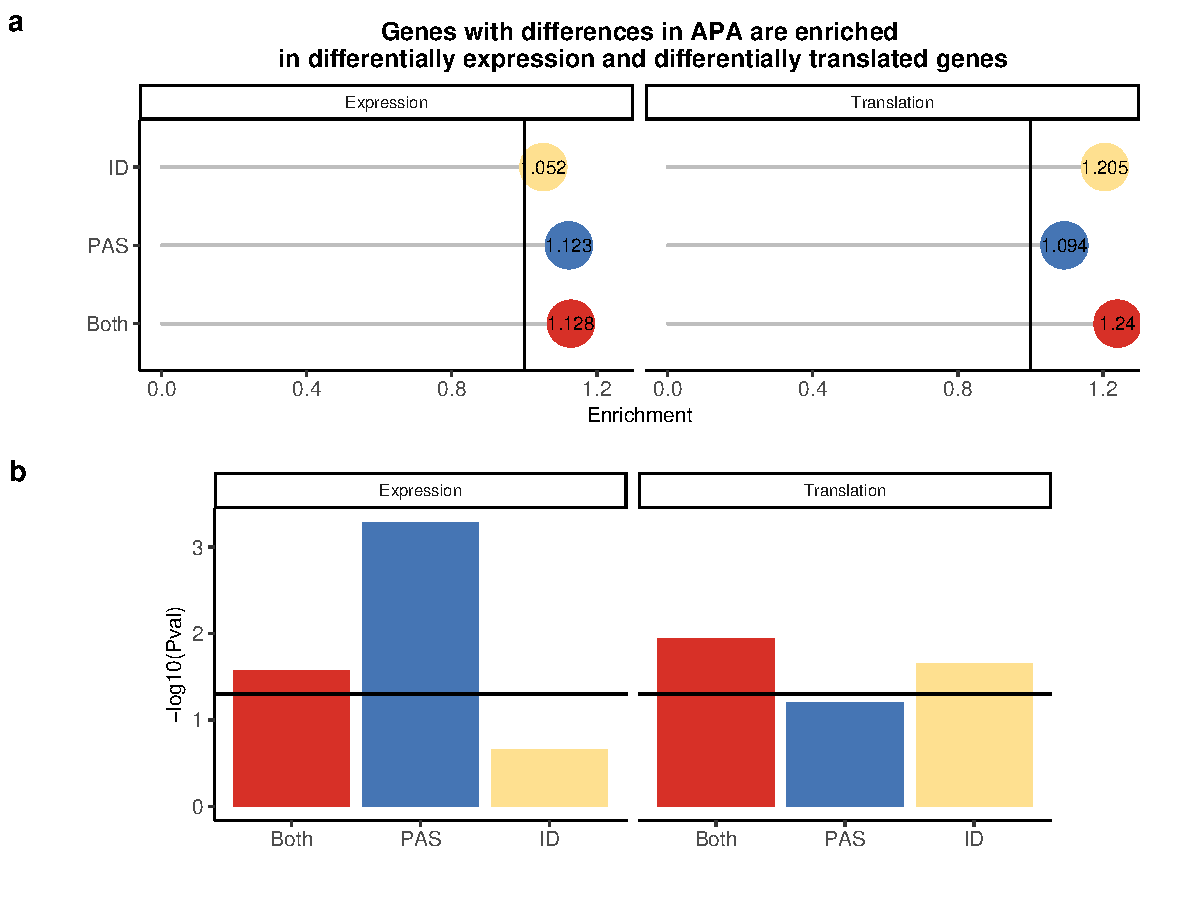
\includegraphics[width=5in]{img/ch03/fig4.pdf}
\caption[Differences dominant PAS site between species likely drives differences in expression]{\textbf{Differences dominant PAS site between species likely drives differences in expression} \small {\bf (A)} Enrichment of genes with the different (left) of same (right) dominant PAS by dominant cutoff in differentially expressed genes. {\bf (B)} $-log_{10}(P-values)$ for enrichments in A calculated with hypergeometric tests. Horizontal line represents p-value of 0.05.} 
\label{fig:Ch3fig4}
\end{figure}


In a previous study that collected mRNA from a larger panel of human, chimpanzee, and rhesus macaque LCLs, Khan \emph{et al.} identified genes whose regulation likely evolves under directional selection in humans and chimpanzees \citep{khan_primate_2013}. We were able to consider RNA and protein expression data as well as APA data from 2,532 genes. We found that twenty-two of the genes with significant inter-species differences in APA at both the site level and in isoform diversity are among those whose regulation likely evolves under directional selection in the chimpanzee lineage, a 1.6X enrichment over what is expected by chance (hypergeometric test, $p=0.015$). We did not find a similar enrichment when we considered genes whose regulation evolved under selection in humans, but the sample size is rather small. 



\subsection{Variation in APA and differences in protein expression}\label{dAPAdp}

Given the well-characterized molecular connection between APA and the regulation of protein translation, we hypothesized that genes with inter-species differences in APA are also more likely to be differentially translated between the species \citep{digiammartino_mechanisms_2011,floor_tunable_2016-1,tian_alternative_2017}. To examine this, we obtained estimates of protein translation based on ribosome profiling data that were collected from human and chimpanzee LCLs by Wang \emph{et al.} \citep{wang_post-translational_2018}. At a 5\% FWER, Wang \emph{et al.} identified 73 differentially translated genes between humans and chimpanzees. Genes with significant inter-species differences in isoform diversity are enriched among the differentially translated gene set ($p = 0.011$; Figure \ref{fig:Ch3fig5}A,B). 

\begin{figure}
\centering
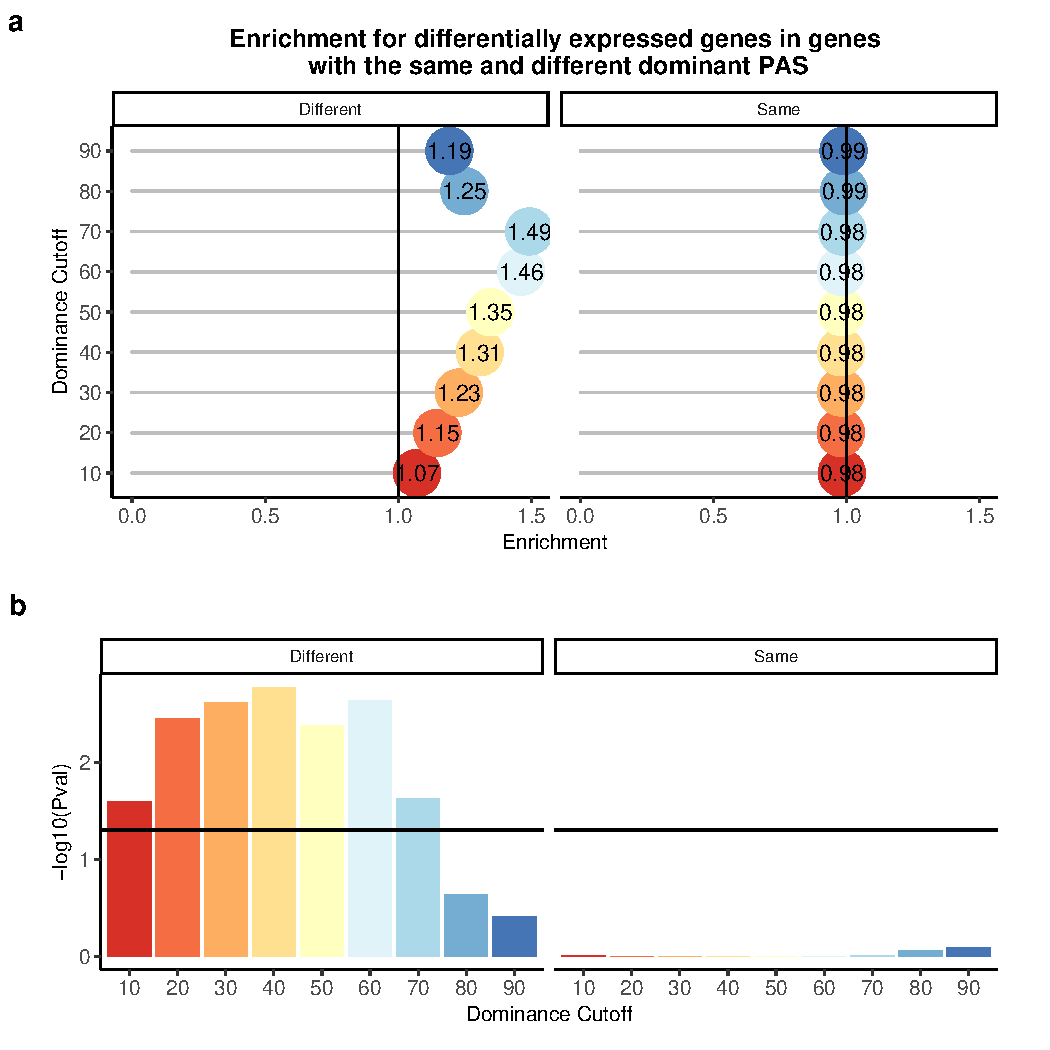
\includegraphics[width=5in]{img/ch03/fig5.pdf}
\caption[PAS level differences in APA may drive differences in expression while isoform diversity differences likely drive translation differences]{\textbf{PAS level differences in APA may drive differences in expression while isoform diversity differences likely drive translation differences} \small {\bf (A)} Enrichment of genes with isoform diversity differences (ID), differences in APA at PAS level (PAS), or at both levels (Both) within differential expressed genes and differentially translated genes. Differentially translated genes reported by Wang \emph{et al.}\citep{wang_post-translational_2018} {\bf (B)} $-log_{10}(P-values)$ for enrichments in A calculated with hypergeometric tests. Horizontal line represents p-value of 0.05.} 
\label{fig:Ch3fig5}
\end{figure}


We next investigated the relationship between $\Delta PAU$ in humans and chimpanzees and the effect sizes for differences in protein translation between the species \citep{wang_post-translational_2018}. Considering the most differentially used 3' UTR or intronic PAS per gene (Methods), we identified a significant correlation between inter-species differences in translation and $\Delta PAU$ for 3' UTR PAS, with a stronger correlation among genes with significant differences in both APA and translation (Supplementary Figure \ref{fig:ch03-TEdAPA}). As expected, and to some extent we view this as a control analysis, we did not identify a significant correlation between intronic PAS $\Delta PAU$ values and differences in translation (Supplementary Figure \ref{fig:ch03-TEdAPA}). 

Given the apparent impact of PAS usage on protein translation, we next considered direct measurements of protein expression data from 3,391 genes in LCLs from humans and chimpanzees \citep{khan_primate_2013}. Using summary statistics from this study, we found 1,263 genes to be differentially expressed at the protein level between the species (FDR of 5\%). As the protein measurements are restricted to these 3,391 genes, we do not have enough power to ask if genes with inter-species differences in APA are also more likely to be differentially expressed at the protein level. However we did find a positive correlation between the absolute value of 3' UTR $\Delta PAU$ and the standardized number of ubiquitination sites for the same gene (Pearson's correlation, $R=0.15$, $p=5.0x10^{-7}$, Supplementary Figure \ref{fig:ch03-ubiq}, Methods), consistent with the observation that 3' UTR PAS are targets for the regulation of protein decay \citep{dubnikov_protein_2017, ravid_diversity_2008}.

Thus, we next focused on the 506  genes with significant inter-species differences in protein expression and an absence of corresponding difference of transcript expression levels that we also tested for differences in APA. Khan \emph{et al.} reasonably hypothesized that inter-species differences in translation could account for the emergence of differences in protein expression levels when there are no regulatory differences at the RNA level, but they were unable to point to specific mechanisms. These genes are particularly interesting in the context of our current study, because APA which results in changes to 3' UTR length may be more likely to result in differences in protein expression without affecting the expression level of the mRNA. 

Indeed, we found 76 genes with inter-species differences in APA that are also differentially expressed at the protein but not at the RNA level between humans and chimpanzees (Figure \ref{fig:Ch3fig6}A,B). In these 76 genes, inter-species differences in PAS usage are enriched at the 3' UTR (Supplementary Figure \ref{fig:ch03-dpnotE}). Finally, to assess whether APA contributes to differences in gene regulation by affecting translation efficiency or protein degradation, we asked whether genes with differential protein expression were also differentially translated. Of the 149 genes with significant differences in APA and protein expression, Wang \emph{et al.} reported translation measurements for 142 \citep{wang_post-translational_2018}. Only 34 genes displayed significant differences in translation efficiency, suggesting that isoform-specific post-translational buffering is largely responsible for protein-level differences (Figure \ref{fig:Ch3fig6}C,D). 


\begin{figure}
\centering
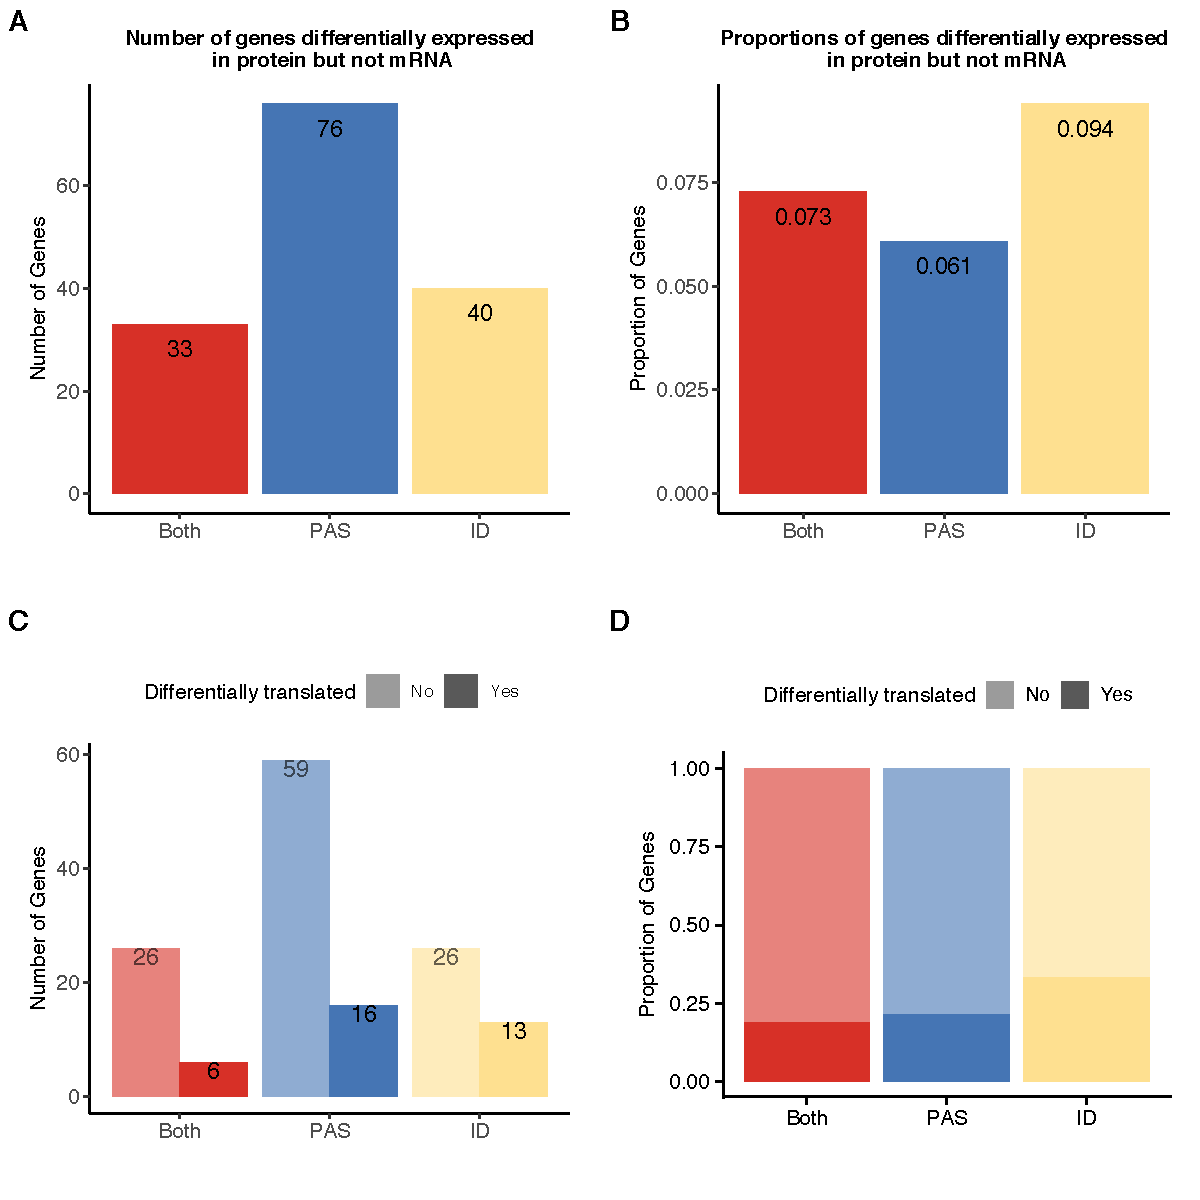
\includegraphics[width=5in]{img/ch03/fig6.pdf}
\caption[APA differences explain genes differentially expressed at protein level but not in mRNA. APA likely mediates functional differences post translationally.]{\textbf{APA differences explain genes differentially expressed at protein level but not in mRNA. APA likely mediates functional differences post translationally.} \small {\bf (A)} Number of genes with isoform level differences (ID), differences in APA at PAS level (PAS), or at both levels (Both) differentially expressed in protein (5\% FDR), but not mRNA (5\% FDR). Genes with differentially expressed protein reported in Khan \emph{et al.} \citep{khan_primate_2013} {\bf (B)} Proportion of genes with differential usage at PAS level (1,251 genes), isoform diversity level (426 genes) or both (454 genes), differentially expressed in protein (5\% FDR), but not mRNA (5\% FDR). {\bf (C)} Genes reported in A separated by genes differentially translated at 5\% FDR. Differentially translated genes reported in Wang \emph{et al.}\citep{wang_post-translational_2018} {\bf (D) } Genes differentially expressed in protein but not in mRNA, colored by differences in APA. Proportion of genes in the set differentially translated at 5\% FDR.} 
\label{fig:Ch3fig6}
\end{figure}



\section{Discussion}


Comparative primate functional genomics studies have contributed to our understanding of the gene regulatory processes that control genotype-phenotype relationships. The general framework starts with non-hypothesis driven research to characterize gene regulatory phenotypes in both human and non-human primates \citep{blekhman_sex-specific_2010,fair_gene_2020}. In comparison to studying a regulatory phenotype in a human population, this approach is useful because, even at modest sample sizes, larger differences between primates make it easier to detect genes with biologically relevant differences \citep{housman_prime_2020}.Once we understand the general properties and level of conservation of individual regulatory phenotypes, we can integrate data collected in the same cell lines or tissues to generate testable hypotheses for how variation in regulatory processes contribute to differences in physical traits. First, identification of genomic regions under adaptation in humans may point to causal mechanisms for human specific traits \citep{gokhman_differential_2020, ward_generally_2019}. Second, identification of heavily conserved genomic regions is critical because mutations in conserved loci likely have negative functional consequences and could be responsible for human disease risk \citep{housman_assessment_2019}. With regard to this general framework, the results above represent the first step in understanding the evolutionary importance of gene regulation though APA. Greater characterization of APA variation in additional cell types will aid in the understanding of how variation percolates through the central dogma as well as how this variation contributes to differences in human traits.  

We characterized alternative polyadenylation in humans and chimpanzees to begin to understand the role that co-transcriptional mechanisms play in the evolution of gene regulation in primates. We focused on the contribution of APA to interspecies differences in transcript and protein expression. Our group has studied a variety of gene regulatory phenotypes in primate LCLs \citep{cain_gene_2011, khan_primate_2013, wang_post-translational_2018, zhou_epigenetic_2014}, and we, and others, have previously demonstrated that gene regulatory phenotypes in these cell lines recapitulate many regulatory patterns seen in primary tissues \citep{caliskan_effect_2014,caliskan_effects_2011,khaitovich_evolution_2006}. Not only did our use of primate LCLs allow us to circumvent many of the practical and ethical issues associated with primate research, but it also allowed us to integrate 3' Seq and gene expression data from this study with previously collected ribosome occupancy and protein expression data from primate LCLs \citep{khan_primate_2013, wang_post-translational_2018}.


APA is an important molecular mechanism with regard to both the evolution of gene regulation and physiological traits. On a long-term evolutionary scale, both 3' UTR length and the proportion of genes exhibiting APA have scaled with genome size and complexity. The expansion of APA has introduced biological complexity independent of an increase in the number of distinct genes \citep{mayr_evolution_2016,mayr_regulation_2017}. As usage of multiple isoforms have been maintained, it is likely that distinct isoforms have divergent functions acted on by balancing selection. For example, APA facilitates post-transcription regulation of a Drosophila Hox gene through maintenance of 2 isoforms differentially targeted by multiple miRNAs \citep{patraquim_evolution_2011}. In terms of physiological traits, genome wide changes in APA during differentiation of stem cells to terminal cell types directs isoform specific gene regulation that is important for development in a range of species, including humans \citep{hilgers_neural-specific_2011, ji_progressive_2009, li_dynamic_2012}. In addition, dysregulation of tumor suppressor genes through intronic polyadenylation is also known to contribute to cancer pathogenesis \citep{dubbury_cdk12_2018,lee_widespread_2018}. We hypothesize that a further understanding of APA in primates will aid in the understanding of APA evolution and its contribution to human specific phenotypes. 


We measured APA from 3' Seq data by calculating a ratio of isoforms terminating at one PAS compared to isoforms terminating at other PAS for the same gene. We then compared PAS usage ratios between species. To expand our understanding of APA conservation, we also calculated an isoform diversity statistic (Simpson's D) for each gene in each species. Because Simpson's D captures both the number of PAS isoforms and their usage, we were able to evaluate small regulatory changes spread across many PAS, rather than simply measure large changes at one PAS. While previous studies have used Shannon's Index to quantify isoform diversity \citep{pai_widespread_2016, wang_post-translational_2018}, we found Simpson's D to be less correlated with PAS number than Shannon's Index, making it less sensitive to the number of PAS per gene (Supplementary Figure \ref{fig:ch03-shanonNum}, \ref{fig:ch03-simpNum}). In addition, by placing more weight on dominant PAS, Simpson's D more closely mirrors our current biological understanding of APA, wherein dominant PAS play a larger role in downstream gene regulation \citep{morris_choosing_2014}.


In general, we found that both individual PAS usage and isoform diversity are highly conserved between human and chimpanzee. Consistent with comparative studies of APA in humans and rodents, which used genomic synteny to identify conserved PAS, we found higher conservation among genes with a single PAS \citep{ara_conservation_2006, wang_compendium_2018} and showed that sequence variation in PAS signal sites and the surrounding U-rich regions contributes to interspecies differences in APA \citep{wang_compendium_2018}. Because we characterized APA in closely related primates, our study provides additional insight into APA divergence at both the gene level and the species level, revealing functional changes that contribute to differences in downstream gene regulation. For example, we observed that when genes use one PAS more often than others, the dominant PAS tends to be the same in both human and chimpanzee. It is likely that strong selection pressures have acted on these genes resulting in continual usage of the same dominant isoform. As a result, we can assume the dominant isoform is functionally important and alternative isoforms would be deleterious. The question remains, why are the non-dominant isoforms also conserved and at what level of expression do the alternative isoforms begin to impede gene function. 

Out study also revealed that the majority of differentially used PAS between species are located in 3' UTRs. We showed that whereas increased intronic PAS usage is associated with increased mRNA expression levels, increased 3' UTR PAS usage is correlated with a decrease in mRNA expression. In a previous study, we found that human apaQTL alleles associated with increased intronic PAS usage were correlated with decreased mRNA expression levels \citep{mittleman_alternative_2020}. We reasoned that transcripts terminating in introns were likely subject to nonstop decay, and by studying APA variation within humans, we were able to capture the effects of intronic termination. Because the current study characterized APA between humans and chimpanzees, such effects were likely overshadowed by interspecies differences, which typically have much larger effect sizes \citep{housman_prime_2020}. Thus, usage of intronic PAS may contribute to down regulation of gene expression in some genes but in others, increased usage of intronic PAS result in truncated isoforms that do not contain 3' UTR cis regulatory elements that would signal mRNA decay. In these cases, the truncated isoforms are no longer targets of mRNA decay, causing certain genes to appear upregulated in RNA-Seq experiments.

As an alternative explanation for the results in this study, large effect sizes for differential usage of 3' UTR PAS could be driving the relationship between differential APA and differential expression. In line with this hypothesis, we pointed to increases in AU destabilizing elements and ubiquitination marks for genes with divergent 3' UTR PAS. Due the ratio nature of PAS usage, we may detect changes in the usage of intronic PAS solely as a mathematical consequence of changes in 3' UTR PAS. Functional follow-up on the genes with PAS detected as differentially used between and within species would be necessary to explore the relative importance of each of these regulatory pathways and to disentangle the results from both studies.

Indeed, APA is not the first molecular phenotype wherein a within-species study revealed alternative regulatory models compared to an interspecies analysis. For example, Pai \emph{et al.} reported tissue-specific differential methylation to be almost exclusively inversely correlated with gene expression patterns between human and chimpanzee \citep{enard_differences_2004, pai_genome-wide_2011, weber_distribution_2007}, whereas Banovich \emph{et al.} discovered genetic variation associated with methylation variation \emph{(meQTLs)} that was both directly and inversely correlated with eQTLs. 


In several previous studies from our group and others, the authors estimated the proportion of variation in expression explained by the regulatory mechanism of interest. Specifically, they tested for differences in expression before and after accounting for another regulatory mechanism with formal mediation analyses \citep{blake_comparison_2020, blekhman_segmental_2009, cain_gene_2011,eres_reorganization_2019}. Similar mediation analyses may have helped us to better understand how usage of intronic and 3' UTR PAS contribute to differences in mRNA expression. However, in our study, APA was measured using ratios of alternative mRNA isoforms. Thus, effect sizes for APA and differential expression are on different scales and we cannot use a mediation approach to formally calculate the proportion of expression variation explained by APA. However, we are generally convinced that APA contributes to differences in mRNA expression overall because 764 of 3,796 (20.1\%) differentially expressed genes also have significant differences in APA. 


Even though genes are ultimately expressed as proteins, many studies measure mRNA expression as a proxy for gene expression. As a justification for this approach, authors point to the fact that after accounting for technical considerations, the correlation between mRNA levels and abundance in quite high genome wide \citep{buccitelli_mrnas_2020,csardi_accounting_2015}. However, we also know that on the level of one gene across individuals or tissues, the correlation between mRNA and protein measurements are much lower \citep{battle_impact_2015,buccitelli_mrnas_2020}. This suggests that a number of molecular mechanisms decouple mRNA and protein levels post transcriptionally. As evident by the fact that we are still unable to predict protein levels from mRNA, we do not fully understand the post transcriptional mechanisms that shape the proteome \citep{buccitelli_mrnas_2020}.

Within human populations and between primates there are large number of genes differentially expressed in mRNA, but not in protein. Directly measuring translation levels for these genes has demonstrated that post-translation protein buffering can explain the decreased variation at the protein level \citep{battle_impact_2015,wang_post-translational_2018}. Conversely there are also genes that are more variable in protein than in mRNA \citep{battle_impact_2015,chick_defining_2016, khan_primate_2013}. Our previous work demonstrated that some protein specific QTLs are also highly correlated with differences in APA \citep{mittleman_alternative_2020}. Here, we expanded this analysis and demonstrated that genes differentially expressed in protein, but not in mRNA between human and chimpanzee, have divergent APA patterns. We also concluded that the divergent protein levels are likely due to post-translational molecular mechanisms. While we cannot directly test the mechanism here, by differentially including RNA and protein binding motifs, APA could leads to variation in protein levels as a consequence of  protein auto-regulation \citep{buccitelli_mrnas_2020,de_bie_ubiquitination_2011, muller-mcnicoll_auto-regulatory_2019}. Alternatively, APA could contribute to temporal and spacial differences for proteins, that would modify our ability to quantify protein with traditional techniques \citep{buccitelli_mrnas_2020,tian_alternative_2017}. In conclusion, a better understanding of co-transcriptional gene regulatory mechanisms, such as APA, may point to additional mechanisms contributing to the decoupling of mRNA and protein abundance.  


\section{Methods}


\subsection{Cell culture and collections}\label{CellCultureColl}

We grew 6 human and 6 chimpanzee Epstein-Bar virus transformed lymphoblastoid cell lines \emph{(LCLs)} in glutamine depleted RPMI [RPMI 1640 1X from Corning (15-040-CM)], completed with 20\% FBS, 2mM GlutaMax [Gibco (35050-061)], 100 IU/ml Penicillin, and 100 ug/mL Streptomycin. We cultured all cells at 37C at 5\% CO2. We passaged each cell line a minimum of 3 times then maintained cells at $1x10^{6}$ cell per mL in preparation for collection. Cell line numbers and details can be found in Table \ref{tab:ch03-s2}. The human lines were derived from Yoruba individuals collected as part of the HapMap project and can be ordered through the Coriell Institute \citep{HapMap2005}. Chimpanzee LCLs were originally transformed from individuals from the New Iberia Research Center (University of Louisiana at Lafayette), Coriell IPBR repository and Arizona State University \citep{khan_primate_2013}. The cell lines have previously been used for similar studies of primate gene regulation \citep{cain_gene_2011, khan_primate_2013, wang_post-translational_2018, zhou_epigenetic_2014}.

Once all cells lines reached $1x10^{6}$ cell per mL, we used the collection and RNA extraction method detailed in Mittleman \emph{et al.} to extract whole cell and nuclear mRNA. Briefly, we collected 30 million cells in two 15 million cell aliquots. We extracted nuclei from one aliquot per line using the nuclear isolation protocol outlined by Mayer and Churchman \citep{mayer_genome-wide_2016}. We extracted mRNA in two fraction- and species-matched batches, using the miRNeasy kit (Qiagen) according to manufacture instructions, including the DNase step to remove genomic DNA. We quantified mRNA and tested quality using a nanodrop. Details of mRNA processing for each line, including concentrations and quality can be found in Table \ref{tab:ch03-s2}. 

\subsection{3' Sequencing to identify PAS and quantify site usage }\label{PASident}

We generated 3' sequencing \emph{(3' Seq)} libraries from whole cell and nuclear-isolated mRNA from 6 chimpanzee and 6 human individuals using the QuantSeq Rev 3' mRNA-Seq Library Prep Kit \citep{moll_quantseq_2014} according to the manufacturer's instructions. We sequenced all libraries on the Illumina NextSeq500 at the University of Chicago Genomics Core facility using single-end 50 bp sequencing.

We mapped human 3' Seq libraries to GRCh38 \citep{schneider_evaluation_2017} and chimpanzee libraries to panTro6 \cite{chimpanzee_sequencing_and_analysis_consortium_initial_2005} using the STAR RNA-seq aligner with default settings \citep{dobin_star_2013}. Similar to our previous work, we removed reads with evidence of internal priming resulting from the poly(dT) primer. We filtered reads proceeded by 6 As or 7 of 10 As in the base pairs directly upstream of the mapped location 
\citep{mittleman_alternative_2020, sheppard_accurate_2013, tian_large-scale_2005}. To ensure that differences in low quality bases would not bias our results, we treated any N in the genome annotation as an A. All raw read counts, mapped read counts, and filtered read counts can be found in Table \ref{tab:ch03-s2}. 

We first identified an inclusive set of PAS in each species separately. We used the same in-house peak caller described in Mittleman \emph{et al} \citep{mittleman_alternative_2020}, annotating each PAS as the most 3' base in each peak. The initial PAS set included 340,023 in human and 303,249 in chimps. We extended PAS 100 bp upstream and 100 bp downstream and used a reciprocal liftover pipeline to identify an inclusive set of orthologous PAS. We downloaded chain files from UCSC genome browser \citep{kent_human_2002}. Details of the pipeline and number of PAS passing each step can be found in Supplementary Figure \ref{fig:ch03-liftover}.

Due to gene annotation differences between species, we annotated all orthologous PAS to the human NCBI RefSeq annotation downloaded from UCSC genome browser \citep{pruitt_ncbi_2005}, We used a hierarchical model to assign PAS to genic locations\citep{lin_-depth_2012, mittleman_alternative_2020}. We prioritized annotations in the following order: 3' UTRs (UTR3), 5kb downstream of genes (end), exons (cds), 5' UTRs (UTR5), and introns (intron). We quantified reads mapping to each annotated PAS for each individual in both the total RNA libraries and nuclear RNA libraries using featureCounts with the -s strand specificity flag \citep{liao_featurecounts_2014}. We calculated usage for each PAS in each library as a ratio of reads mapping to the PAS divided by the number of reads mapping to any PAS in the same gene (Supplementary Figure \ref{fig:ch03-UsageCalc}). We implemented two filtering steps to remove PAS with ratios likely biased by low site count or low gene count separately in each fraction.

Next, we filtered out sites with less than 5\% usage in both species in the nuclear fraction. We then merged nuclear counts across all PAS in each gene. We removed PAS in genes not passing a cutoff of $log_{2}(CPM)>2$ in at least 8 of the 12 individuals. After applying these filters, we were left with 44,432 PAS. As a quality control metric, we compared PAS usage calculated from the nuclear fraction to PAS usage calculated from whole cell fraction for each individual (we used the same methods to identify and quantify PAS usage in the whole cell 3' Seq data). We expected a high correlation between PAS usage in each fraction. Further, we expected a similar correlation in human and chimpanzee individuals \citep{mittleman_alternative_2020}. Human individual NA18499 had significantly lower across-species correlation than the other individuals and was therefore removed from the analysis (Supplementary Figure \ref{fig:ch03-removeInd}. 


 To ensure gene expression level did not introduce ascertainment bias, we tested the relationship between PAS number and normalized gene expression. In both species, number of PAS is negatively correlated with normalized gene expression (Human: Pearson's correlation =-0.19, $p< 2.2x10^{-16}$, Chimp: Pearson's correlation=-0.17, $p< 2.2x10^{-16}$, Supplementary Figure \ref{fig:ch03-PASexp}). We expected species to contribute the most amount of variation to PAS usage. We ran PCA on the filtered nuclear PAS usage. PC1 accounts for 41.8\% of the variation and is highly correlated with species ($R^{2} =0.68$). PC2 accounts for 13.1\% of the variation and is moderately correlated with RNA extraction technician ($R^{2}=0.38$) and extraction day ($R^{2}=0.28$). As both of these variables are balanced with respect to species, we do not believe they bias the results (Supplementary Figure \ref{fig:ch03-PCAthreeprime}). We identified 302 sites used at a rate of 5\% in humans and 0\% in chimpanzees, which we designated as human-specific. We identified 357 sites used at a rate of 5\% in chimpanzee and 0\% in humans, which we designated as chimp-specific. 
 
 We acknowledge the possibility that unlifted PAS may affect downstream analyses; therefore, we removed genes for which PAS ratios may be affected. Specifically, we annotated and calculated usage for the human PAS, including the 10,077 PAS that do not reciprocally lift to the chimpanzee genome. After removing PAS in genes previously identified as lowly expressed and PAS with usage below 5\%, 386 PAS in 353 genes remain (Supplementary Figure \ref{fig:ch03-unlift}). We removed these 353 genes and recreated Figures \ref{fig:Ch3fig3},  \ref{fig:Ch3fig4},  \ref{fig:Ch3fig5},  \ref{fig:Ch3fig6} (Supplementary Figures \ref{fig:ch03-unliftfig3},  \ref{fig:ch03-unliftfig5}, \ref{fig:ch03-unliftfig4}, \ref{fig:ch03-unliftfig6}).
 
\subsection{Orthologous 3' UTRs}\label{OrthoUTR}
 
 We identified a set of orthologous UTRs using the ortho exon file described the Differential Expression section of the methods. We merged all regions annotated as 3' UTR by gene. If a gene had multiple non-continuous annotations, we selected the most 3' region as the orthologous UTR. We used deepTools compute matrix and plotHeatmap functions to plot merged human and chimpanzee reads along the orthologous 3' UTR set (Supplementary Figure \ref{fig:ch03-deeptools}, \citep{ramirez_deeptools2_2016}) For all genes with PAS only in 3' UTRs, we assigned PAS to single, first, middle, and last, as previously described \citep{wang_compendium_2018}.
 
\subsection{Analysis of sequence conservation around PAS}\label{seqCons} 

We used phyloP scores to measure sequence level conservation. We downloaded the hg38 100-way vertebrate PhyloP bigwig file from the UCSC table browser \citep{pollard_detection_2010}. We computed scores for PAS regions as well as 200 bp intervals by taking the mean of the base pair scores. We removed any region with missing data from the analysis.  We tested for differences in mean phloP scores using Wilcoxon rank sum tests. 


We tested for presence of the polyadenylation signal site motif in the 200 bp PAS regions. We used the bedtools nuc tool with the strand-specific flag to test for presence of each of the 12 previously annotated motifs for each PAS in both species \citep{beaudoing_patterns_2000, quinlan_bedtools_2010}. If a PAS had multiple motifs, we used a hierarchical model to choose the site based on the number of PAS with each identified motif (order: AATAAA, ATTAAA, AAAAAG, AAAAAA, TATAAA, AATATA, AGTAAA, AATACA, GATAAA, AATAGA, CATAAA, ACTAAA). The proportion of PAS with each signal site motif matched across species (Figure \ref{fig:Ch3fig1}). To ask if presence or absence of a signal site explained species specificity or site-level differences, we restricted our analysis to the top two signal sites. These two motifs are the only sites where presence of a signal is associated with increased usage of the site in both species (Supplementary Figure \ref{fig:ch03-SignalUsage}). For the 359 PAS with one of these two signal sites present only in chimpanzees, average usage was higher in chimpanzees than in humans ($p=0.025$). For the 361 PAS with one of these two signal sites present only in humans, average usage was higher in humans ($p=2.0x10^{-4}$). We used hypergeometric tests to evaluate enrichment of differentially used PAS and species-specific PAS in the set of PAS with signal sites in only one species.

We also examined the proportion of U nucleotides in each PAS region. We used the bedtools nuc with the -s flag for strand specificity \citep{quinlan_bedtools_2010}. We tested if PAS with differences in U content are enriched for differentially used PAS using a hypergeometric test. 


\subsection{Differential APA}\label{dAPA} 

\emph{PAS level differences:} We quantified reads mapping to each PAS using the featureCounts tool with the -s strand specificity tool \citep{liao_featurecounts_2014}. We tested for site-level differences between human and chimpanzee using the leafcutter leafcutter\_ds.R tool with standard settings \citep{li_annotation-free_2018}. We tested for differences in both the total and nuclear fractions. We tested 43,038 PAS in 8,422 genes in the nuclear fraction and 41,914 PAS in 8,333 genes in the total fraction. We classified PAS as differentially used if the gene reached significance at 5\% FDR and the PAS had a $\Delta PAU$ greater than 20\% (absolute value ($\Delta PAU > 0.2$). A negative $\Delta PAU$ indicates increased usage in chimpanzees and $\Delta PAU$ indicates increased usage in humans. Top PAS per gene is the PAS with the most significant difference between species; ties were broken using mean usage for all individuals in both species. 

\emph{Isoform diversity differences:} We calculated Shannon Information content ( $- \sum_{i=1}^{S} p_{i}log_{2}p_{i}$ ) and Simpson's Index ($1 - \sum_{i=1}^{S} p^{2}_{i}$) using mean usage of each PAS in humans and chimpanzees, where $p_{i}^{2}$ is the usage of the $i^{th}$ of $s$ sites in the gene. We used Simpson's Index to assess isoform diversity because the correlation between Simpson's Index and number of PAS is lower than the correlation between Shannon Information content and the number of PAS per gene (Supplementary Figure \ref{fig:ch03-shanonNum}, \ref{fig:ch03-simpNum}). To identify genes with differences in isoform diversity, we recalculated Simpson's index per gene per individual and tested for differences between species with Wilcoxon tests. We reported genes with differences at 5\% FDR.  

\emph{Conservation of dominant PAS:}  We consider a gene to have a dominant PAS if the within species average usage of the top used PAS is greater than the second most used site by an arbitrary cutoff. We reported results for cutoffs between 0.1 and 0.9. If a gene had a dominant PAS in either species, we included the top used site for both species when testing if genes use the same or different dominant PAS between species. We tested for enrichment of genes using the same or different dominant PAS with differentially expressed genes using hypergeometric tests.

\subsection{Differential expression analysis}\label{dE} 
 
We generated unstranded RNA-seq libraries using the Illumina TruSeq Total RNA kit according to the manufacturer's instructions using the total mRNA collected from all 12 individuals (Illumina, San Diego, CA, USA). We sequenced RNA-seq libraries at the University of Chicago Genomics Core facility using the single-end 50 bp protocol on one lane of the Illumina HiSeq 4000 machine. RNA quality and concentration at the time of library prep and number of sequenced reads per library are available in  Table \ref{tab:ch03-s3}. We mapped the human libraries to GRhg38 \citep{schneider_evaluation_2017} and chimpanzee libraries to panTro6 \citep{chimpanzee_sequencing_and_analysis_consortium_initial_2005} and quantified reads mapping to orthologous exons. 

To generate an updated orthologous exon file for the most recent chimpanzee genome assembly \emph{(panTro6)} we followed the procedure reported in Pavlovic \emph{et al.} with slight modifications \citep{pavlovic_comparative_2018}. We started with human \emph{(GRCh38)} exon definitions from Ensembl version 98. We filtered this set of definitions for biotypes 'protein\_coding,' using the command mkgtf from cellranger (10XGenomics). We then removed exon segments that were in exon definitions for multiple genes. This broke some exons into smaller unique exons. We then removed exons smaller than 10 bp. We took the final set of exons (1,371,917 exons from 20,338 genes) and extracted their sequences from the genome Ensembl GRCh38.p12. We used BLAT V. 35 to identify orthologous sequences within the chimpanzee genome \emph{(panTro6)} \citep{kent_human_2002} We removed hits with indels larger than 25 bp (using a function blatOutIndelIdent from \url{https://bitbucket.org/ee_reh_neh/orthoexon}). We then extracted the panTro6 sequences that had the highest sequence identity. We ran BLAT on this orthologous exon set to find matches in both the human and chimpanzee genomes. We removed exons that did not return the original location in humans or chimpanzees, as well as exons that mapped to multiple places with higher than 90\% sequence identity. We removed exons that different human genes that mapped to overlapping regions in the chimpanzee genome. Finally, we removed exons that mapped to a different contig than the majority of exons from each gene. This resulted in a set of 1,250,820 orthologous exons from 19,515 genes. 

We mapped on average 18.6 million reads to orthologous exons. We collapsed orthologous exons to quantify raw gene expression for each gene in each individual. We standardized counts and filtered out genes without $log_{2}(CPM)$ values greater than 1 in 8 of the 12 individuals. To prepare counts for differential expression modeling we used the Voom function with the quantile normalization method in the limma R package \citep{ritchie_limma_2015}. We used PCA to test for batch effects. PC1 explains 35.1\% of the variation and is highly correlated with species ($R^{2}= 0.98$) (Supplementary Figure \ref{fig:ch03-DEQC}). Collected metadata such as the percent of live cells at collection, cell concentration at collection, RIN score, and RNA concentration do not segregate by species (Supplementary Figure \ref{fig:ch03-DEQC}). We modeled species as a fixed effect and called genes as differentially expressed at a 5\% FDR. The results from our differential expression analysis, including effect sizes and significance values are available in Table \ref{tab:ch03-s4}. 



\subsection{Integration of translation and protein data}\label{dTdP} 

We downloaded differential translation genes and effect sizes from Additional file 5 of Wang \emph{et al}\citep{wang_post-translational_2018}. Wang \emph{et al.} modeled differential translation using ribosome profiling of 4 human, 4 chimpanzee, and 4 rhesus macaque LCLs. For all integrations, we conditioned on the 6,407 genes tested in the Wang \emph{et al.} study and in our APA analysis. We tested for enrichments using a one-sided hypergeometric test implemented in R. We tested for correlations in effect sizes between site level $\Delta PAU$ and translation HvC effect sizes by first filtering for the top PAS (see top PAS method above, Supplementary Figure \ref{fig:ch03-TEdAPA}). We report Pearson's correlations calculated in R. 

We downloaded differential protein level genes, effect sizes, and directional selection classifications from table S4 of Khan \emph{et al.}\citep{khan_primate_2013}. Khan \emph{et al.} modeled differential protein expression of 3,390 genes using high resolution mass spectrometry of stable isotope labeling by amino acids in cell culture \emph{(SILAC)} collected from 5 human, 5 chimpanzee, and 5 rhesus macaque LCLs. 

\subsection{Supplemental functional data}\label{supFunc}

We downloaded human protein length (in number of amino acids) for proteins annotated as reviewed for high confidence from UniProtKB \citep{the_uniprot_consortium_uniprot_2019}. We downloaded ubiquitination protein modification data from PhosphoSitePlus version 050320 \citep{hornbeck_phosphositeplus_2015}. For all analyses in which we used interaction or ubiquitination data, we normalized the values by number of amino acids. To identify 3' UTR AU-rich elements in human RefSeq annotated 3' UTRs, we used the transcriptome\_properties.py script published in Floor and Doudna 2016, available at \url{https://github.com/stephenfloor/tripseq-analysis}, with the -au-elements flag \citep{floor_tunable_2016-1}. According to Floor and Doudna 2016, the fraction of AU-elements is the percentage of the 3' UTR with repeating AU elements of 5nt or more\citep{floor_tunable_2016-1}.

\subsection{Data and code
availability}\label{ch03-data-and-code-availability} All scripts and analysis pipelines can be found at \url{https://brimittleman.github.io/Comparative_APA/index.html.} FastQ files and PAS annotations are available on GEO under GSE155245. 

\section{Acknowledgments}\label{ch03-acknowledgments}
We thank N. Gonzales for comments on the manuscript. We thank Y. Li, M. Ward, and G. Housman for useful discussion.  Funding: This work was supported by the US National Institutes of Health (RO1 to Y.G). B.E.M. supported by T32 GM09197 to the University of Chicago and F31HL149259 to B.E.M. from National Heart, Lung, And Blood Institute of the National Institutes of Health. SP was in part supported by the National Center for Advancing Translational Sciences of the NIH (K12 HL119995). This work was completed in part with resources provided by the University of Chicago Research Computing Center.
 
\section{Author Contributions}\label{ch03-author-contributions}
B.E.M. conceived the project with help from Y.G and S.P. B.E.M., S.W., C.C. and S.P. performed the experiments. B.E.M performed the analysis. K.B. curated orthologous exon file. B.E.M. drafted the manuscript with input from Y.G. and S.P. S.P. and Y.G supervised the project.


\clearpage

\section{Supplementary Information}\label{ch03-supplementary-information}

\subsection{Supplementary Figures}\label{ch03-supplementary-figures}

\clearpage

\begin{figure}[!htb]
\centering
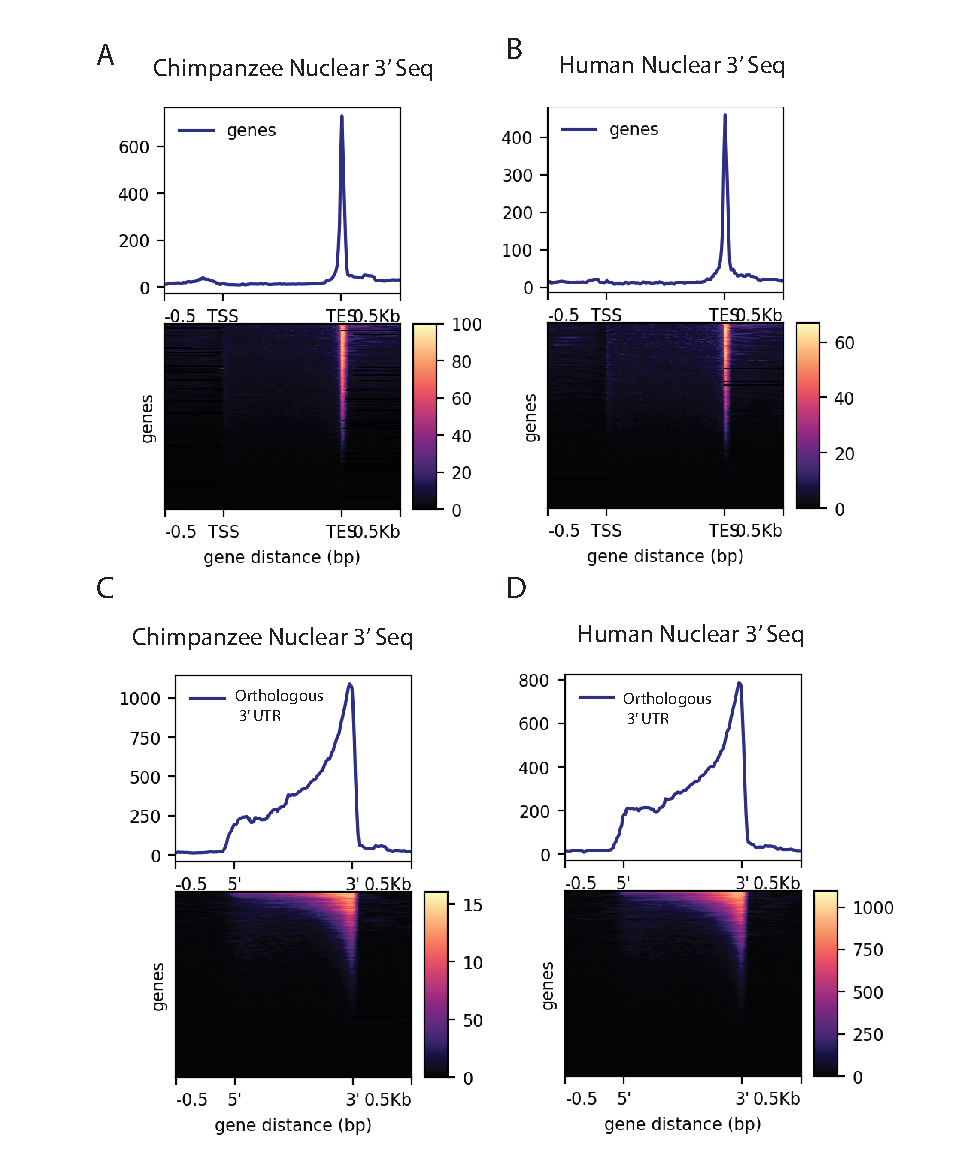
\includegraphics[width=5in]{img/ch03/Fig1-figSup1.pdf}
\caption[Density of merged human and chimpanzee 3' Seq]{\textbf{Density of merged human and chimpanzee 3' Seq} {\bf (A)}  Coverage of 6 chimpanzee, nuclear 3' seq reads along Refseq transcripts {\bf (B)}  Coverage of 5 human, nuclear 3'seq reads along Refseq transcripts {\bf (C)}  Coverage of 6 chimpanzee, nuclear 3' seq reads orthologous 3' UTRs {\bf (D)} Coverage of 5 human, nuclear 3' seq reads orthologous 3' UTRs}
\label{fig:ch03-deeptools}
\end{figure}
\clearpage

\begin{figure}[!htb]
\centering
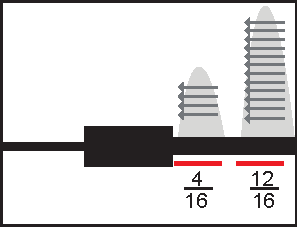
\includegraphics[width=5in]{img/ch03/Fig1-figSup2.pdf}
\caption[Model representation of usage calculation]{\textbf{Model representation of usage calculation} Representation of PAS usage calculation. Usage is a ratio of reads at each PAS to the number of reads mapping to any PAS in the same gene. Adapted from Chapter \ref{ch:QTL}}
\label{fig:ch03-UsageCalc}
\end{figure}
\clearpage

\begin{figure}[!htb]
\centering
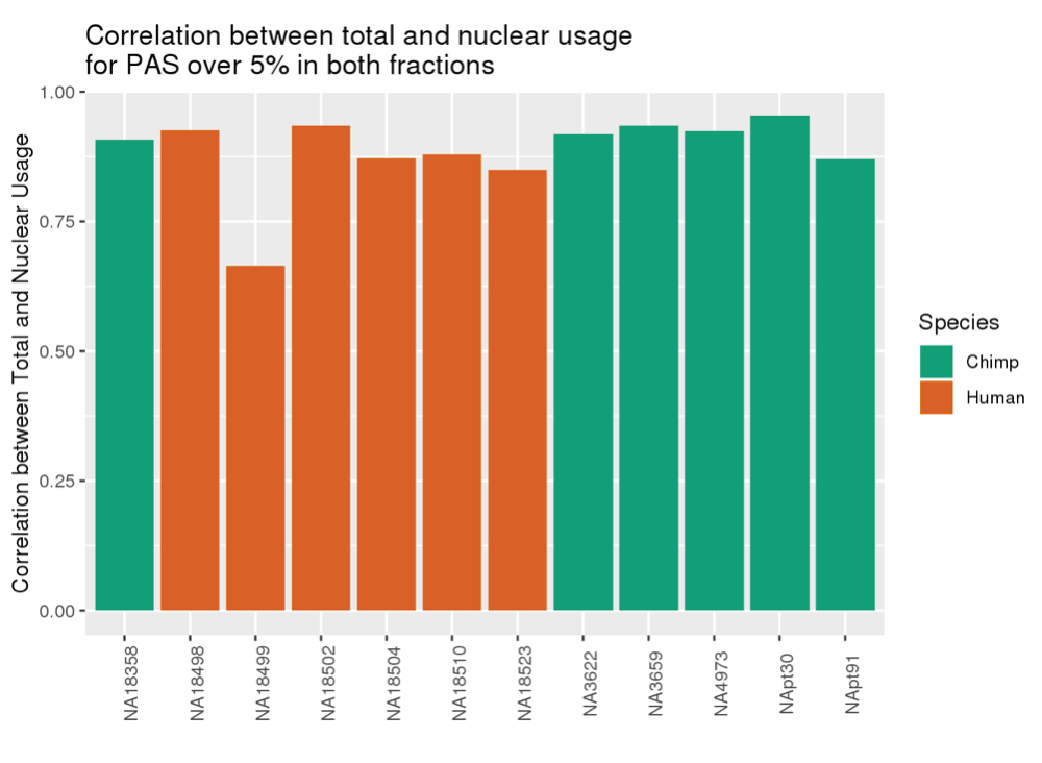
\includegraphics[width=5in]{img/ch03/Fig1_figSup11.pdf}
\caption[NA18499 removed from analysis due to low correlation between fractions]{\textbf{NA18499 removed from analysis due to low correlation between fractions} Pearson's correlation between PAS usage calculated using nuclear 3' seq libraries and total mRNA 3' seq libraries, calculated using sites reaching 5\% in one species in both fractions. (Plot from previous commit 30ff122 on Aril 9, 2020). }
\label{fig:ch03-removeInd}
\end{figure}
\clearpage

\begin{figure}[!htb]
\centering
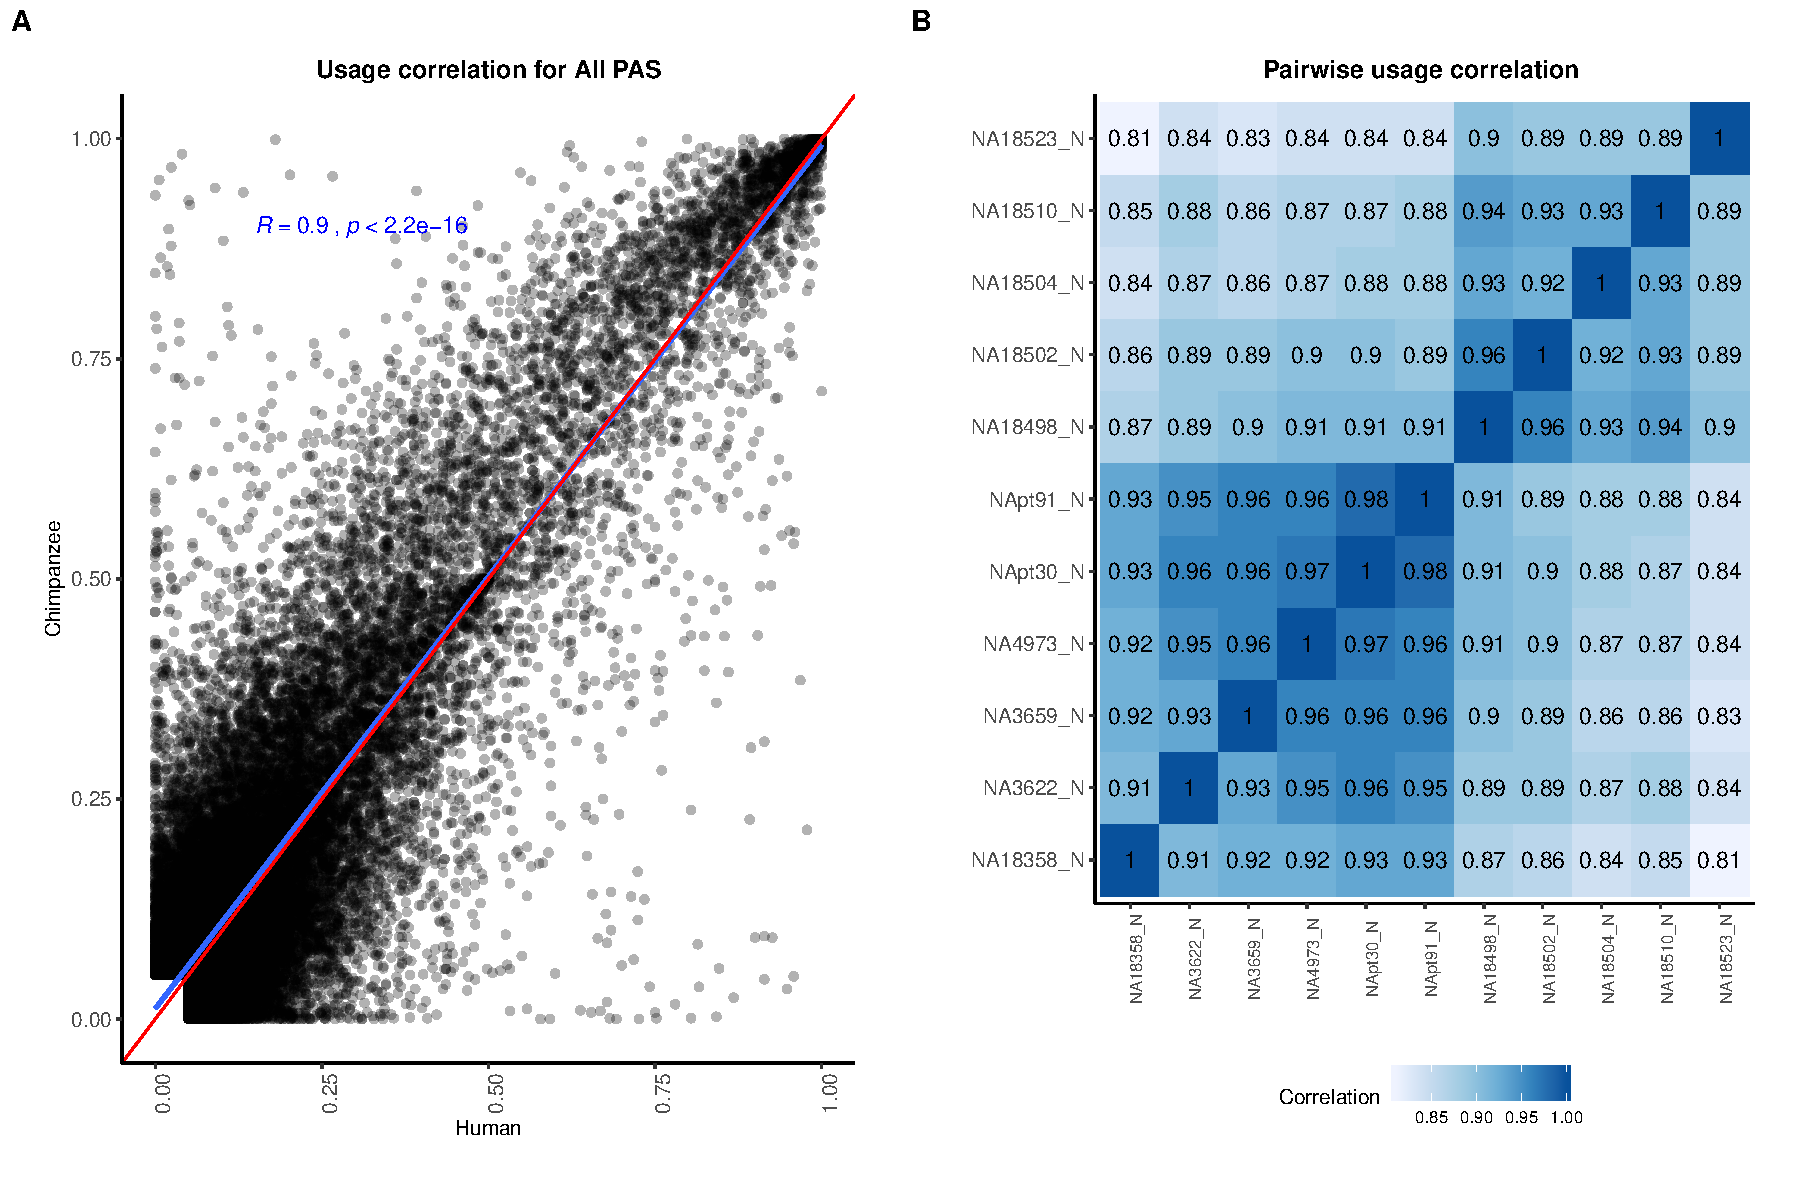
\includegraphics[width=5in]{img/ch03/Fig1-figSup3.pdf}
\caption[PAS usage is highly correlated across species]{\textbf{PAS usage is highly correlated across species} {\bf (A)}  Correlation between human and chimpanzee PAS usage for 44,432 PAS. Red line is a 1:1 line. Linear regression line and Pearson's correlation plotted in blue. {\bf (B)}  Pairwise correlation for human and chimpanzee PAS usage.}
\label{fig:ch03-UsageCorr}
\end{figure}
\clearpage

\begin{figure}[!htb]
\centering
\includegraphics[width=5in]{img/ch03/Fig1-figSup4.pdf}
\caption[Variation in PAS usage]{\textbf{Variation in PAS usage} {\bf (A)}  Plot of first two principal components \emph{(PCs)} calculated by a principal component analysis on PAS usage (44,432 PAS). Chimpanzee samples are shown in red and human samples are shown in blue {\bf (B)}  Heatmap representing correlation between technical factors and PCs. Y axis factors include: Species, Extraction date, Collection person, AverageAlive (average of two live dead calculations at time of collection), RIN score, RNA concentration. Explanation of factors and values in Table \ref{tab:ch03-s1}}
\label{fig:ch03-PCAthreeprime}
\end{figure}
\clearpage


\begin{figure}[!htb]
\centering
\includegraphics[width=5in]{img/ch03/Fig1-figSup5.pdf}
\caption[PAS detection likely not biased by expression level]{\textbf{PAS detection likely not biased by expression level} {\bf (A)}  Normalized gene expression plotted against the number of PAS detected at 5\% usage in chimpanzee. {\bf (B)}  Normalized gene expression plotted against the number of PAS detected at 5\% usage in human.  The R package ggpubr was used to plot linear regression lines and calculate Pearson's correlations.}
\label{fig:ch03-PASexp}
\end{figure}
\clearpage


\begin{figure}[!htb]
\centering
\includegraphics[width=5in]{img/ch03/Fig1-figSup6.pdf}
\caption[PAS detection likely not biased by species]{\textbf{PAS detection likely not biased by species} Histogram of the number of PAS detected at 5\% usage in human minus the number of 5\% usage in chimpanzees. Red vertical line represents mean difference (0.39).}
\label{fig:ch03-SpecPASnum}
\end{figure}
\clearpage


\begin{figure}[!htb]
\centering
\includegraphics[width=5in]{img/ch03/Fig1-figSup7.pdf}
\caption[Figure 1B separated by genic location]{\textbf{Figure 1B separated by genic location} Mean PhyloP scores for PAS regions (yellow) and 200 base pair bins upstream and downstream of PAS (orange). A one-sided Wilcoxon test was used to test for increased PhyloP in PAS regions  (Coding region: $p < 2.2x10^{-16}$, 5 kb downstream of genes: $p = 7.02x10^{-6}$, intron: $p=0.99$, 3' UTR: $p < 2.2x10^{-16}$, 5' UTR: $p = 0.011$).}
\label{fig:ch03-phylopLoc}
\end{figure}
\clearpage

\begin{figure}[!htb]
\centering
\includegraphics[width=5in]{img/ch03/Fig1-figSup8.pdf}
\caption[PAS with AATAAA and ATTAAA are used more often]{\textbf{PAS with AATAAA and ATTAAA are used more often} Mean PAS usage of the top two signal site motifs in human and chimpanzee plotted by annotated signal site.}
\label{fig:ch03-SignalUsage}
\end{figure}
\clearpage

\begin{figure}[!htb]
\centering
\includegraphics[width=5in]{img/ch03/Fig1_figSup9.pdf}
\caption[Chimp specific PAS likely due to loss of signal site in human lineage]{\textbf{Chimp specific PAS likely due to loss of signal site in human lineage} {\bf (A)} IGV track for example of a chimpanzee specific PAS in MAN2B2 gene. Top track is merged coverage from 5 human nuclear 3' seq libraries. Chimp track is merged coverage from 6 chimpanzee nuclear 3' seq libraries lifted to human genome with CrossMap\citep{zhao_crossmap_2014} {\bf (B)}  Sequence alignment for region upstream of proximal PAS from UCSC genome browser\citep{kent_human_2002}. Black box indicates the signal site location. Canonical signal site is the ancestral state and was lost in the human lineage.}
\label{fig:ch03-exChimpspec}
\end{figure}
\clearpage

\begin{figure}[!htb]
\centering
\includegraphics[width=5in]{img/ch03/Fig2-figSup1.pdf}
\caption[Genic Location of PAS differentially used between human and chimpanzee]{\textbf{Genic Location of PAS differentially used between human and chimpanzee} Differentially used PAS (5\% FDR) between human chimpanzee by genic annotation.}
\label{fig:ch03-dPAS}
\end{figure}
\clearpage

\begin{figure}[!htb]
\centering
\includegraphics[width=5in]{img/ch03/Fig2-figSup2.pdf}
\caption[Location of PAS within Orthologous 3' UTRs]{\textbf{Location of PAS within Orthologous 3' UTRs} Proportion of sites differentially used or conserved by whether they are the first (yellow), middle (blue), or last PAS (red) in orthologous exons. }
\label{fig:ch03-whichUTR}
\end{figure}
\clearpage

\begin{figure}[!htb]
\centering
\includegraphics[width=5in]{img/ch03/Fig2_figSup3.pdf}
\caption[Genes with differentially used PAS are enriched for genes with apaQTL ]{\textbf{Genes with differentially used PAS are enriched for genes with apaQTL} 10,000 random subsamples of genes tested for differential APA and overlap with genes with apaQTLs from Chapter \ref{ch:QTL}. Red line represents the actual overlap between genes with differential usage of at least one PAS and apaQTL genes.}
\label{fig:ch03-dPASQTL}
\end{figure}
\clearpage


\begin{figure}[!htb]
\centering
\includegraphics[width=5in]{img/ch03/Fig3-figSup1.pdf}
\caption[Figure 3.3 relationships expanded to total usage]{\textbf{Figure 3.3 relationships expanded to total usage} {\bf (A)}  Total mRNA  $\Delta PAU$ for top intronic or 3' UTR PAS per gene plotted against differential effect size from differential expression analysis. {\bf (B)} Total mRNA $\Delta PAU$ for top intronic or 3' UTR PAS per gene plotted against differential effect size from differential expression analysis for genes with significant differences in each phenotype at 5\% FDR. {\bf (C)} Total mRNA $\Delta PAU$ for top intronic or 3' UTR PAS per gene plotted against differential effect size from differential expression analysis. {\bf (D)} Total mRNA $\Delta PAU$ for top intronic or 3' UTR PAS per gene plotted against differential effect size from differential expression analysis for genes with significant differences in each phenotype at 5\% FDR. In all panels, I calculated the linear regression and Pearson's correlation with the r package ggpubr. In B and D, I  colored the points and regression line by genic location. In all panels, negative $\Delta PAU$ and DE effect sizes represent upregulation in chimpanzees.}
\label{fig:ch03-totalDPASDE}
\end{figure}
\clearpage


\begin{figure}[!htb]
\centering
\includegraphics[width=5in]{img/ch03/Fig2-figSup4.pdf}
\caption[Information content measurement densities]{\textbf{Information content measurement densities} {\bf (A)}  Density of Shannon indices for all tested genes in human and chimpanzee ( $- \sum_{i=1}^{S} p_{i}log_{2}p_{i}$ ) {\bf (B)}  Density of Simpson indices for all tested genes in human and chimpanzee ($1 - \sum_{i=1}^{S} p^{2}_{i}$)  }
\label{fig:ch03-bothDensities}
\end{figure}
\clearpage


\begin{figure}[!htb]
\centering
\includegraphics[width=5in]{img/ch03/Fig2-figSup5.pdf}
\caption[Relationship between Shannon index and PAS number ]{\textbf{Relationship between Shannon index and PAS number} Shannon information index plotted against the number of PAS detect for each gene. Pearson's correlation and significance in black. }
\label{fig:ch03-shanonNum}
\end{figure}
\clearpage

\begin{figure}[!htb]
\centering
\includegraphics[width=5in]{img/ch03/Fig2-figSup6.pdf}
\caption[Relationship between Simpson diversity index and PAS number]{\textbf{Relationship between Simpson diversity index and PAS number} Simpson's diversity index plotted against the number of PAS detect for each gene. Pearson's correlation and significance in black.}
\label{fig:ch03-simpNum}
\end{figure}
\clearpage

\begin{figure}[!htb]
\centering
\includegraphics[width=5in]{img/ch03/Fig2_figSup7.pdf}
\caption[Intersection between genes with PAS and isoform diversity differences]{\textbf{Intersection between genes with PAS and isoform diversity differences} 1251 genes have significant differences in PAS usage at between human and chimpanzee (left). 454 genes have significant differences in APA between humans and chimpanzee in PAS usage and in isoform diversity (middle). 427 genes with differences in isoform diversity level only (right).}
\label{fig:ch03-upsetr}
\end{figure}
\clearpage



\begin{figure}[!htb]
\centering
\includegraphics[width=5in]{img/ch03/Fig4_figSup1.pdf}
\caption[Gene with significant differences in isoform diversity only]{\textbf{Gene with significant differences in isoform diversity only} Human and chimpanzee usage for 5 PAS identified in the IVNS1ABP gene. None of the PAS measured have significant differences in usage at 5\% FDR. IVNS1ABP is not differentially expressed.}
\label{fig:ch03-ivn}
\end{figure}
\clearpage

\begin{figure}[!htb]
\centering
\includegraphics[width=5in]{img/ch03/Fig4-figSup2.pdf}
\caption[Relationship between $\Delta PAU$  and differential translation effect sizes]{\textbf{Relationship between $\Delta PAU$  and differential translation effect sizes} {\bf (A)} $\Delta PAU$ for top 3' UTR and intronic PAS plotted against differential translation \emph{(TE)} effect size as reported by Wang \emph{et al.}\citep{wang_post-translational_2018} {\bf (B)} $\Delta PAU$ for top 3' UTR and intronic PAS plotted against TE effect size as reported by Wang \emph{et al.} \citep{wang_post-translational_2018} separated by genic location.  {\bf (C)} $\Delta PAU$ for top 3' UTR and intronic PAS with significant differences in usage plotted against TE effect size for significant genes (5\% FWER) as reported by Wang \emph{et al.}\citep{wang_post-translational_2018}. {\bf (D)}  $\Delta PAU$ for top 3' UTR and intronic PAS with significant differences in usage plotted against TE effect size for significant genes (5\% FWER) as reported by Wang \emph{et al.}\citep{wang_post-translational_2018} separated by genic location. Linear regression line was plotted and Pearson's correlation was calculated for data in each panel.}
\label{fig:ch03-TEdAPA}
\end{figure}
\clearpage

\begin{figure}[!htb]
\centering
\includegraphics[width=5in]{img/ch03/Fig3-figSup2.pdf}
\caption[Relationship between APA differences and protein decay mark]{\textbf{Relationship between APA differences and protein decay mark} {\bf (A)} Absolute value of $\Delta PAU$ for 3' UTR PAS with significant difference at site level plotted against the number of ubiquitination marks in the gene standardized by the number of amino acids. Regression line and Pearson's correlation are plotted in red.{\bf (B)} Absolute value of $\Delta PAU$ for intronic PAS with significant difference at site level plotted against the number of ubiquitination marks in the gene standardized by the number of amino acids. Regression line and Pearson's correlation are plotted in blue.}
\label{fig:ch03-ubiq}
\end{figure}
\clearpage

\begin{figure}[!htb]
\centering
\includegraphics[width=5in]{img/ch03/Fig6-figSup1.pdf}
\caption[Enrichment for 3' UTR PAS in genes differentially expressed in protein and not in mRNA]{\textbf{Enrichment for 3' UTR PAS in genes differentially expressed in protein and not in mRNA} Genic location enrichments for the PAS in genes differentially expressed at protein level but not mRNA level among all differentially used PAS. Pvalues were calculated with a hypergeometric test.}
\label{fig:ch03-dpnotE}
\end{figure}
\clearpage


\begin{figure}[!htb]
\centering
\includegraphics[width=5in]{img/ch03/Fig1_figSup10.pdf}
\caption[Reciprocal liftover pipeline]{\textbf{Reciprocal liftover pipeline} Reciprocal liftover pipeline for unfiltered PAS including the number of sites remaining at each step. Liftover using UCSC liftover tool and chain files downloaded from UCSC genome browser \citep{kent_human_2002}. }
\label{fig:ch03-liftover}
\end{figure}
\clearpage


\begin{figure}[!htb]
\centering
\includegraphics[width=5in]{img/ch03/Fig2-figSup8.pdf}
\caption[PAS that do not lift from human to chimp]{\textbf{PAS that do not lift from human to chimp} Of the 10,077 PAS that do not reciprocally lift from human to chimp, distribution of where sites are filtered out. Most are lost due to not mapping to genes or due to low usage (likely noise). }
\label{fig:ch03-unlift}
\end{figure}
\clearpage

\begin{figure}[!htb]
\centering
\includegraphics[width=5in]{img/ch03/Fig3-figSup3.pdf}
\caption[Figure 3.3 without genes affected by liftover]{\textbf{Figure 3.3 without genes affected by liftover} {\bf (A)} $\Delta PAU$ for top intronic or 3' UTR PAS per gene plotted against differential effect size from differential expression analysis.  {\bf (B)}  $\Delta PAU$ for top intronic or 3' UTR PAS per gene plotted against differential effect size from differential expression analysis for genes with significant differences in each phenotype at 5\% FDR. {\bf (C)}  $\Delta PAU$ for top intronic or 3' UTR PAS per gene plotted against differential effect size from differential expression analysis. {\bf (D)}  $\Delta PAU$ for top intronic or 3' UTR PAS per gene plotted against differential effect size from differential expression analysis for genes with significant differences in each phenotype at 5\% FDR. In all panels, I calculated the linear regression and Pearson's correlation with the r package ggpubr. In B and D, I  colored the points and regression line by genic location. In all panels, negative $\Delta PAU$ and DE effect sizes represent upregulation in chimpanzees.}
\label{fig:ch03-unliftfig3}
\end{figure}
\clearpage


\begin{figure}[!htb]
\centering
\includegraphics[width=5in]{img/ch03/Fig5-figSup1.pdf}
\caption[Figure 3.4 without genes affected by liftover]{\textbf{Figure 3.4 without genes affected by liftover} {\bf (A)}  Enrichment of genes with the different (left) or same (right) dominant PAS by dominant cutoff in differentially expressed genes after removing genes likely affected by liftover. {\bf (B)} $-log_{10}(p-values)$ for enrichments in A calculated with hypergeometric tests. Horizontal line represents $p= 0.05$.}
\label{fig:ch03-unliftfig5}
\end{figure}
\clearpage

\begin{figure}[!htb]
\centering
\includegraphics[width=5in]{img/ch03/Fig4-figSup3.pdf}
\caption[Figure 3.5 without genes affected by liftover]{\textbf{Figure 3.5 without genes affected by liftover} {\bf (A)} Enrichment of genes with differences in isoform diversity, PAS usage, or both within differential expressed genes and differentially translated genes after removing genes likely affected by liftover. Differentially translated genes reported by Wang \emph{et al.}\citep{wang_post-translational_2018}. {\bf (B)}  $-log_{10}(p-values)$ for enrichments in A calculated with hypergeometric tests. Horizontal line represents $p= 0.05$.}
\label{fig:ch03-unliftfig4}
\end{figure}
\clearpage


\begin{figure}[!htb]
\centering
\includegraphics[width=5in]{img/ch03/Fig6-figSup2.pdf}
\caption[Figure 3.6 without genes affected by liftover]{\textbf{Figure 3.6 without genes affected by liftover} {\bf (A)} Number of genes with differences in isoform diversity, PAS usage or both differentially expressed in protein (5\% FDR) but not in mRNA (5\% FDR). Genes differentially expressed in protein from Khan \emph{et al.}\citep{khan_primate_2013} {\bf (B)} Proportion of genes with differential isoform diversity, PAS usage or both that are differentially expressed in protein (5\% FDR), but not mRNA (5\% FDR). {\bf (C)} Genes reported in separated by genes differentially translated at 5\% FDR. Differentially translated gene reported in Wang \emph{et al.}\citep{wang_post-translational_2018}. {\bf (D)} Genes differentially expressed in protein but not in mRNA, colored by differences in APA. Proportion of genes in the set differentially translated at 5\% FDR.}
\label{fig:ch03-unliftfig6}
\end{figure}
\clearpage


\begin{figure}[!htb]
\centering
\includegraphics[width=5in]{img/ch03/Fig3_figSup4.pdf}
\caption[Differential expression quality control plots]{\textbf{Differential expression quality control plots} {\bf (A)} First two principal components \emph{(PCs)} in gene expression variation. {\bf (B)} Heatmap representing correlation between technical factors and PCs. Explanation of Y axis factors and values available in Table \ref{tab:ch03-s2} {\bf (C)} Percent of live cells as calculated by trypan blue staining at collection is not confounded by species. {\bf (D)}  RIN scores reported by bioanalyzer at RNA-seq library generation are not confounded by species.{\bf (E)}  RNA concentrations reported by bioanalyzer at RNA-seq library generation are not confounded by species. {\bf (F)}  Cell concentrations at time of collection are not confounded by species.}
\label{fig:ch03-DEQC}
\end{figure}
\clearpage


\clearpage
\section{Supplementary Tables}\label{ch03-supplementary-tables}

\begin{table}[!htb]
\caption[PAS differential usage]{\textbf{PAS differential usage} 
(see supplementary file associated with this dissertation) Differential PAS usage results. Column names as described- PAS: polyadenylation site, gene: gene (cluster in leafcutter), PAS\_logeffectsize: log effect size for differential usage of the PAS between human and chimpanzee, PAS\_deltaPAU: difference in polyadenylation site usage between human and chimpanzee (delta PSI in leafcutter), Gene\_lohLR: log likelihood ratio for differential usage of any PAS in the gene. (cluster likelihood ratio in leafcutter), Gene\_adjustedPvalue: adjusted pvalue for differential usage of the any PAS in the gene (cluster pvalue in leafcutter)}
\label{tab:ch03-s1}
\end{table}



\begin{table}[!htb]
\caption[3' Seq metadata]{\textbf{3' Seq metadata} 
(see supplementary file associated with this dissertation) Metadata for 3' Seq data. Column names as described- Species:Cell line species , Lines: Cell line ID, Fraction: Cellular fraction, CollectionDate: Date of cell harvest and nuclear isolation, Extraction\_date: Date of RNA extraction, Collection\_person: Author initial for who processed cell harvest and nuclear isolation, UndilutedAverage: Average of 2 cell count measurements $1x10^6$, AverageAlive: Average of 2 cell live dead counts - calculated with trypan blue stain, Concentration: Extracted RNA concentration (ng/ml), RIN: RIN score for extracted RNA, 260.280.Ratio: 260/280 ratio calculated on nanodrop, Library: 3' Seq library date, Reads: Number of sequenced reads, Mapped\_wMP: Number of Mapped reads before removing reads likely due to misprimming, Mapped\_Clean: Number of Mapped reads after removing reads likely due to misprimming}
\label{tab:ch03-s2}
\end{table}


\begin{table}[!htb]
\caption[RNA sequencing metadata]{\textbf{RNA sequencing metadata} 
(see supplementary file associated with this dissertation) Metadata for RNA sequencing data. Column names as described- Species:Cell line species , Lines: Cell line ID, Collection\_person: Author initial for who processed cell harvest and nuclear isolation, UndilutedAverage: Average of 2 cell count measurements $1x10^6$, AverageAlive: Average of 2 cell live dead counts - calculated with trypan blue stain, CollectionDate: Date of cell harvest and nuclear isolation, Extraction: Date of RNA extraction,  RIN: RIN score for extracted RNA, BioAConc: RNA concentration (ng/ul), Reads: Number of Sequenced reads, Mapped: Number of mapped reads, AssignedOrtho: Number of mapped reads assigned to orthologous exons.}
\label{tab:ch03-s3}
\end{table}

\begin{table}[!htb]
\caption[Differential expression results]{\textbf{Differential expression results} 
(see supplementary file associated with this dissertation) Differential expression results from limma. gene: tested gene, logFC: log 2 fold change in normalized gene expression, adj.P.Val: BH adjusted pvalue from t test, B: Beta value, t: t statistic }
\label{tab:ch03-s4}
\end{table}





% Chapter 04
\chapter{Native Elongating Transcript sequencing to measure Polymerase II elongation rate in a human population}\label{ch:netseq}

\section{Abstract}\label{ch04-abstract}


In chapter 4, I describe a project in which we aimed to use Native Elongating transcript sequencing (NET-seq) to quantify polymerase II (PolII) elongation speed variation genome wide in a panel of YRI LCLs. Our goal was to map genetic variation associated with PolII elongation speed. We would then ask if these genetic variants were also correlated with previously identified regulatory phenotypes, such as gene expression and alternative splicing. Unfortunately, the NET-seq data was not of high enough quality or complexity to continue the analysis. While this work will not be published elsewhere, the work contributed to my development as a scientist and is thus included here. In this chapter, I will describe our motivation, efforts made, and suggest alternative approaches that may allow for the detection of genetic variation association PolII pausing.  



\clearpage

\section{Introduction}\label{ch04-introduction}

Functional regulatory QTL studies have successfully uncovered a large number of interacting regulatory mechanisms likely responsible for variation in gene expression within human populations \citep{li_rna_2016, McVicker2013, degner_dnase_2012, gaffney_dissecting_2012, battle_genomic_2015}. Such studies have primarily focused on identification of pre-transcriptional gene regulatory features, such as enhancers and promoters, through characterization of chromatin accessibility and histone modifications. However, many of the genetic variants correlated with variation in gene expression fall outside of promoter and enhancer regions.  


Through a meta-analysis of previously characterized molecular phenotypes in the same panel of human lymphoblastoid cell lines Li et al. quantified the proportion of eQTLs with a suggested molecular mechanism. Namely, Li et al, estimated that 60\% of the eQTLs previously identified in LCLs, likely contribute to differences in expression through variation at chromatin level features. This analysis left around 40\% of eQTLs mechanistically unexplained \citep{li_rna_2016}. The unexplained variants lie within gene bodies and were associated with regions of active transcription elongation, suggesting they act through co-transcriptional mechanisms. 

It is likely that genetic variation associated with co-transcriptional mechanisms also contribute to isoform specific gene regulation. mRNA isoform variation arises through alternative splicing and alternative polyadenylation. Genetic variant associated with alternative splicing (sQTLs) and alternative polyadenylation (apaQTLs) are also likely driven by co-transcriptional gene regulation \citep{li_rna_2016, mittleman_alternative_2020}. In turn, a more thorough characterization of co-transcriptional gene regulatory mechanisms could improve our understanding of eQTL, sQTLs, and apaQTLs. 


Using estimates of nascent transcription and polymerase II (PolII) density, researchers have discovered that PolII moves along gene bodies at a non-uniform rate \citep{mayer_native_2015,nojima_mammalian_2015, mahat_base-pair-resolution_2016, day_comprehensive_2016, jonkers_genome-wide_2014}. Specifically, PolII density increases proximal to the promoter, at intron exon boundaries, and at the transcription end site (TES) suggesting PolII pauses at each of these locations during transcription \citep{adelman_promoter-proximal_2012, zeitlinger_rna_2007,rahl_c-myc_2010}.  According to studies in human and other model systems, PolII pausing is tightly regulated \citep{nojima_mammalian_2015, carrillo_oesterreich_global_2010, proudfoot_transcriptional_2016,gromak_pause_2006}. While, various studies have mechanistically implicated PolII dynamics in alternative splicing and APA, there is still debate surrounding causal relationships and the degree to which PolII pauses or simply slows down \citep{price_transient_2018,reimer_rapid_2020}. Moreover, despite the large body of molecular work, no study has quantified interindividual variation in PolII elongation rate. 

We suspect genetic variation contributing to differences in PolII elongation rate are also associated with differences in gene expression, alternative splicing, and alternative polyadenylation. By identifying these genetic variants (pauseQTLs) we can expand our knowledge of gene regulatory mechanisms. We collected Native Elongation Transcript sequencing (NET-seq) data from a population of human lymphoblastoid cell lines (LCLs) in order to quantify variation in PolII density as an estimate of PolII elongation rates. We intended to map genetic variation associated with elongation differences to ask if PolII elongation rate is a co-transcriptional gene regulatory mechanism contributing to variation in gene expression, alternative splicing, and alternative polyadenylation. Unfortunately, this project was not completed as intended because the NET-seq data was not complex enough to assess individual level variation genome wide. 


\section{Results}\label{ch04-results}


A number of protocols have been developed to measure PolII density and nascent transcription genome wide \citep{wissink_nascent_2019}. For this project, we decided to use the Nascent Elongating Sequencing (NET-seq) protocol published by Andreas Mayer and L. Stirling Churchill in 2016 \citep{mayer_genome-wide_2016}. The protocol maps PolII density genome wide at single-nucleotide precision without cell perturbation or nascent RNA labeling. 

We optimized NET-seq for 16 human lymphoblastoid cell lines (LCLs). First, we halted transcription with $\alpha$-Amanitin and purified nascent mRNA molecules from purified chromatin (Figure \ref{fig:ch04-protocol}, panel I-III). We added a DNA linker with a 6 base pair unique molecule identifier (UMI) to the 3' hydroxyl group of each nascent molecule. This step allows for base pair and strand specific detection of individual molecules during downstream bioinformatic steps. After using a gel extraction to select 30-100 nucleotide RNA fragments, we created circular cDNA from each fragment. Because some mature mRNAs, such as snoRNAs remain associated with chromatin and likely contribute to the cDNA pool, we used biotinylated DNA oligos to specifically deplete a number of previously annotated, snRNAs, snoRNAs, rRNAs, and mitochondrial tRNAs. The remaining set of cDNA?s required a fairly high number of PCR amplification cycles (12-20) to achieve libraries with concentrations high enough to sequence. (Figure \ref{fig:ch04-protocol}, panel IV).

\begin{figure}
\centering \includegraphics[trim=0 .5in 0
  0,clip,width=5in]{img/ch04/Figure1.pdf}
\caption[Graphical representation of NET-seq protocol]{\textbf{ Graphical representation of NET-seq protocol published in Mayer et al. \citep{mayer_native_2015}}  {\bf Panel I:} Halt transcription in cells with $\alpha$-Amantin. {\bf Panel II:} Purify chromatin containing PolII. {\bf Panel III:}  Purify nascent mRNA from chromatin fractionation. {\bf Panel IV:}  Library construction by adding DNA linker to 3' OH group, cDNA synthesis, and removal of mature mRNA contaminates}
\label{fig:ch04-protocol}
\end{figure}


\begin{figure}
\centering \includegraphics[trim=0 .3in 0
  0,clip,width=5in]{img/ch04/Figure2.pdf}
\caption[Quality control metrics for NET-seq libraries.]{\textbf{Quality control metrics for NET-seq libraries.} {\bf A} Histogram of mapped read lengths for NET-seq library NA18486. {\bf B} Histogram of mapped read lengths for NET-seq library NA18508. {\bf C} Histogram of mapped read lengths for NET-seq library NA19238. {\bf D} Histogram of mapped read lengths for NET-seq library generated from HEK cells and published in Mayer et al \citep{mayer_native_2015}). {\bf E} Pearson correlations for NET-seq library coverage in gene bodies. Coverage calculated as number of reads mapping to gene standardized by gene length.}
\label{fig:qualCont}
\end{figure}

We sequenced the libraries to an average depth of 160 million reads. For many libraries, less than 50\% of the reads mapped to the genome and once deduplicated based on UMIs, less than 5\% of sequenced reads were usable. Over 50\% of reads did not map because they were too short. Mapped reads from our libraries were shorter reads than those previously published (\citep{mayer_native_2015}, Figure \ref{fig:qualCont}A-D)


We next evaluated the mapped data on a genome wide scale. We assessed our data using the following metrics introduced by Meyer et al (mayer 2015). At the gene coverage level, NET-seq libraries were highly correlated (Figure \ref{fig:qualCont}E). Overall, we observed a bias toward read coverage at the 5' end of gene bodies (methods, Figure \ref{fig:genecov}A).  Within genes, we observed enrichment at 5' and 3' exon boundaries for the top 5\% of expressed exons (Figure \ref{fig:genecov}B, methods). After standardizing the number of reads mapping to each gene by gene length only, on average 42.7\% of genes were detected at greater than 0.001 standardized reads (Figure \ref{fig:genecov}C). Given the average gene length, 0.001 standardize reads represented about 65 reads. 


\begin{figure}
\centering \includegraphics[trim=0 .3in 0
  0,clip,width=5in]{img/ch04/Figure3.pdf}
\caption[NET-seq Gene coverage.]{\textbf{NET-seq Gene coverage.} {\bf A} Enrichment for Distribution of read coverage along gene bodies calculated with Picard tools (NA18505, NA18508, NA18486, NA19239, NA19239, NA19141, NA19193, NA19257, NA19128). {\bf B}Histogram and smoothed density plots for NET-seq read coverage at 5' and 3' splice sites. {\bf C} Proportion of genes in each NET-seq library with greater than 0.001 standardized reads (methods).}
\label{fig:genecov}
\end{figure}


Our goal was to identify genomic regions with evidence for high PolII density and map genetic variation associated with variation in PolII elongation rate. In turn, we next explored coverage at individual gene loci. We used a wavelet-based Empirical Bayes shrinkage method implemented in smashr to denoise genic signal (\citep{xing_flexible_2016}, methods). For ACTB, the smoothing allowed us to identify regions of likely Pol II pausing at the TSS and splice sites (Figure \ref{fig:smash}). 



\begin{figure}
\centering \includegraphics[trim=0 .3in 0
  0,clip,width=5in]{img/ch04/Figure4.pdf}
\caption[Smoothing of NET-seq data using smashr ]{\textbf{Smoothing of NET-seq data using smashr \citep{xing_flexible_2016}.} {\bf A} Raw counts along ACTB gene locus for 8 combined libraries (NA18505, NA18508, NA18486, NA19239, NA19239, NA19141, NA19193, NA19257, NA19128) as well as each library separately. {\bf B} Smoothed coverage along ACTB on combined NET-seq data. Signal at 5' and 3' splice sites.}
\label{fig:smash}
\end{figure}
 
Smoothing to differentiate signal from random noise would not account for contamination by mature mRNAs or technical mapping errors. We found evidence of many genomic locations, such as in the INSIG2 gene, with heavy read buildup. We were unable to identify technical or biological reasons for the high density of NET-seq reads (Figure \ref{fig:insig}). We hypothesize that unannotated chromatin associated mRNAs or low complexity repetitive reads. The protocol includes depletion of chromatin associated mature mRNAs, however the oligo pool is likely incomplete. Unannotated snoRNAs or snRNAs likely contribute to high density regions. Alternatively, because mapped reads are relatively short, repetitive genomic regions may be mipmapping, therefore contributing to regions of high read density. 

\begin{figure}
\centering \includegraphics[trim=0 .3in 0
  0,clip,width=5in]{img/ch04/Figure5.pdf}
\caption[NA18486 NET-seq coverage along INSIG2 locus]{\textbf{NA18486 NET-seq coverage along INSIG2 locus}}
\label{fig:insig}
\end{figure}

We did not continue the analysis beyond these quality control metrics and low-level analyses. Further optimization of this protocol or another protocol is likely necessary to quantify Pol II pause pattern variation genome wide. 



\section{Discussion}\label{ch04-discussion}


By extracting and sequencing nascent chromatin-associated mRNA, we attempted to measure polymerase II (PolII) density and estimate transcription elongation rates a population of human LCLs. Using data from 16 individuals we were able to capture the broad patterns previously described by Mayer et al and others \cite{mayer_native_2015}. We found evidence for Poll II pausing at the TSS and at the 5' and 3' splice sites for highly expressed exons. We showed that in genes with high coverage, an Empirical Bayes shrinkage method could differentiate between regions of high PolII density and background random noise. Unfortunately, for most genes, we did not have high enough coverage to smooth the data. Further, we identified regions of the genome where a large proportion of the reads mapped for unknown technical reasons or biological contamination of mature chromatin associated mRNAs.

We believe the NET-seq libraries were of low quality and complexity for a number of reasons. The NET-seq protocol was difficult to optimize due to low concentration of input mRNA. Specifically, we needed to extract chromatin associated mRNA from 8 collections of 15 million cells to achieve the required 1$\mu g$ of input RNA. Moreover, the protocol included multiple gel extraction steps where lot of the mRNA was lost. While we explored alternative options, such as size selection with columns, none were specific enough for the desired fragments. Even after optimizing the protocol to achieve libraries of high enough concentration for sequencing, the nascent RNA fragments were shorter than reads published in Mayer et al \cite{mayer_native_2015}. We believe that while we selected the optimal fragment lengths, shorter fragments were preferentially incorporated and amplified into libraries. 

It is difficult to determine if our libraries were of lower quality than those published in Mayer et al because the published libraries also had a large number of un-mapped reads and a low signal-to-noise ratio. The authors largely characterized patterns across multiple genes did not collect a population sample to identify variation. It is likely that sequencing coverage played a large role in the differences between our results and those reported in Mayer et al \cite{mayer_native_2015}. For one replicated of HEK293T, they sequenced 1.2 billion reads with 555 million uniquely mapping. At this coverage, only 50\% of the reads had coverage of over 1 read per kilobase per million (RPKM) \cite{mayer_native_2015}. While we acknowledged that sequencing to this depth would be unreasonable in a population sample, we planned to take advantage of shared genotypes to identify genetic variants associated with PolII patterns. Unfortunately, our low coverage libraries were too noisy to confidently quantify PolII density, even if we merged on genotypes. 

We still believe that mapping genetic variants associated with PolII density would likely help in our understanding on gene regulation. There are a variety of alternative methods to collect nascent mRNA or PolII associated transcripts. Other potential methods largely fall into two classes. The first category relies on immunoprecipitation of PolII or a specific post translationally modified version of PolII \citep{nojima_mammalian_2015, gariglio_clustering_1981, buck_chip-chip_2004, kim_high-resolution_2005,wissink_nascent_2019, mayer_pause_2017}. These methods potentially suffer from non-specific binding of anti-bodies, and with the exception of mNetseq, are restricted to 200bp resolution \citep{nojima_mammalian_2015}. The second class of approaches utilize in-vitro incorporation of labeled nucleotides to identify regions of transcription potential. Transcription run-on assays, such as GRO-seq and PRO-seq, are vulnerable to variation in experimental conditions because the protocols include stopping and restarting transcriptions in non-physiological conditions \citep{kwak_precise_2013,core_analysis_2014, tome_single-molecule_2018, gardini_global_2017,mahat_base-pair-resolution_2016, mayer_pause_2017, wissink_nascent_2019}. 


To date, only one preprint has reported the usage of a variant of one of these methods to characterize nascent RNA in a population of human cell lines. $Kristj\grave{a}nsd\grave{o}ttir$ et al, quantified 5' capped nascent transcripts in 67 YRI LCLs with PRO-cap \citep{kristjansdottir_population-scale_2018}. In contrast to our work, these authors aimed to characterize transcription at enhancers and to identify genetic variation associated with enhancer transcription initiation. The authors also collected PRO-seq for 10 unique individuals \citep{kristjansdottir_population-scale_2018}. It is possible that once published, we or others could use these data to test for genetic variation associated with co-transcriptional PolII density variation. 


\section{Methods}\label{ch04-methods}



\subsection{Cell culture of LCLs}\label{cell-culture-of-LCLs} 

We cultured 16 human Epstein-Bar virus transformed lymphoblastoid cell lines (LCLs) in glutamine depleted RPMI (RPMI 1640 1X from Corning (15-040-CM)), completed with 15\% FBS, 2mM GlutaMax (Gibco (35050-061)), 100 $IU/ml$ Penicillin, and 100 $\mu g/mL$ Streptomyocin. We cultured all cells at 37C at 5\% CO2. The 16 cell lines represent a subset of the YRI individual LCLs collected as part of the hapmap project and are available through Coriell \citep{HapMap2005}. 
We used lines NA19527, NA19239, NA19238, NA19225, NA19223, NA19209, NA19193, NA19128, NA19141, NA19128, NA18853, NA18508, NA18505, NA18501, NA18497, NA18486. These lines also represent a subset of those used for the 3' sequencing published in Chapter 2 and in Mittleman et al. \citep{mittleman_alternative_2020}. 


\subsection{Collections and library preparation}\label{Collections-and-library-preparation}

After growing the LCLs to around 1 million cells per ml, we separated $1.5x10^{7}$ cells into 10 tubes, one for total cells, one for nuclear fraction and eight for the chromatin fraction. Collection dates and details can be found in Mittleman et al. Additional File 2 \cite{mittleman_alternative_2020}. We used the Native Elongating Transcript sequencing (NET-seq) collection protocol published in Mayer and Churchman 2016 with minor adjustments to three buffers \citep{mayr_evolution_2016}. Specifically, we added 1M $MgCl_{2}$ and 100\% Glycerol to the Cytoplasmic lysis buffer, Sucrose buffer, and the Nuclei wash buffer. We added the $MgCl_{2}$ to stabilize the nucleus and the glycerol as a freezing protectant. We halted transcription with $\alpha$-amanatin and separated the nuclear fraction using mild detergent and a sucrose cushion. We then separate the nucleoplasm from the chromatin using urea, salt, and a mild detergent. We then collected the chromatin through centrifugation and degradation of the DNA with a DNase treatment. We used the Qiagen miRNAeasy kit with manufacture instructions to extract mRNA from all three fractions.


We generated NET-seq library according to the Mayer and Churchman protocol with custom oligos ordered from IDT \citep{mayr_evolution_2016}. I captured the 3' end of chromatin associated mRNA molecules with a barcoded linker and convert the fragments into cDNA for library preparation. We sequenced each NET-seq library at the University Genomics Core facility using single end 50bp sequencing on the Illumina HiSeq4000 machine. We multiplexed 8 libraries together and sequenced each group on a total of 3 lanes. Custom sequencing primers can be found in Mayer and Churchman protocol \citep{mayr_evolution_2016}. 


\subsection{Data processing}\label{Data-processing}



We mapped all NET-seq libraries to GRCH37.75 downloaded from Ensemble using subjunc with default settings \citep{international_human_genome_sequencing_consortium_initial_2001, Liao2013} We used umi\_tools extract to extract the 6 base UMIs and umi-tools dedup to collapse duplicate reads \citep{smith_umi-tools_2017}. 
 
 We assessed computed genome coverage at basepair resolution using bedtools genomecov with the -d and -5 flags. We measured the coverage density along the gencode.v19 gene annotation using picard CollectRnaSeqMetrics \citep{frankish_gencode_2019,quinlan_bedtools_2010}. We used featureCounts with the -T 5 flag to quantify reads within the gencode.v19 gene annotation \citep{frankish_gencode_2019, Liao2014}. We used pysam to extract mapped read statistics from bam files \citep{Li2009}. We downloaded the HEK NET-seq published in Mayer et al. available from GEO under accession number GSE61332 \cite{mayer_genome-wide_2016}.  We re-processed the fastq file using our mapping pipeline. We used the smash.pois function with the EM algorithm in the smashr package on individual genes for signal denoising \citep{xing_flexible_2016}. The function implemented a wavelet-based Empirical Bayes shrinkage method \citep{xing_flexible_2016}. 

We attempted to recreate a version of Mayer et al. figure 7 using NA18486 sequence coverage for this analysis \cite{mayer_genome-wide_2016}. Due to low library coverage and complexity, we did not separate the exons into, constitutive, alternatively retained, alternative skipped. We quantified coverage at base pair resolution for 40bp upstream and downstream of the 5' and 3' splice sites of the top 5\% covered exons. We then standardized base pair coverage by exon coverage.   



% Chapter 05
\chapter{Conclusion}\label{conclusion}

\section{A joint Bayesian model provides a general framework for analyzing functional genomics studies with many conditions}



\section{Initial success classifying individuals susceptible to tuberculsosis and future directions}

\section{Incorporating lessons from single cell pilot study for future studies of the genetic basis of gene expression noise and the response to bacterial infection}


\section{The importance of mitigating batch effects in any genomics experiment}

\section{Concluding remarks}



% Format a LaTeX bibliography
\makebibliography

% Figures and tables, if you decide to leave them to the end
%\input{figure}
%\input{table}

\end{document}


